\documentclass[12pt]{article}

% Paquetes básicos
\usepackage[utf8]{inputenc}
\usepackage[spanish, es-tabla]{babel}
\usepackage{float}
\usepackage{indentfirst}
\usepackage{graphicx}

% Paquetes matemáticos
\usepackage{amsmath}
\usepackage{mathrsfs}
\usepackage{amsfonts}

% Paquetes de formato
\usepackage{vmargin}
\usepackage{multirow}
\usepackage{enumitem}
\usepackage[hidelinks]{hyperref}
\usepackage{hhline}
\usepackage{tikz}

% Paquetes para algoritmos
\usepackage{algorithm}
\usepackage{algpseudocode}

% Paquetes para código
\usepackage{listings}
\definecolor{codegreen}{rgb}{0,0.6,0}
\definecolor{codegray}{rgb}{0.5,0.5,0.5}
\definecolor{codepurple}{rgb}{0.58,0,0.82}
\definecolor{backcolour}{rgb}{0.95,0.95,0.92}
\lstdefinestyle{CStyle}{ 
    backgroundcolor=\color{backcolour},   
    commentstyle=\color{codegreen},
    keywordstyle=\color{magenta},
    numberstyle=\tiny\color{codegray},
    stringstyle=\color{codepurple},
    basicstyle=\footnotesize,
    breakatwhitespace=false,         
    breaklines=true,                 
    captionpos=b,                    
    keepspaces=true,                 
    numbers=left,                    
    numbersep=5pt,                  
    showspaces=false,                
    showstringspaces=false,
    showtabs=false,                  
    tabsize=2,
    language=C
}

% Configuración de página
\setpapersize{A4}
\setmargins{2.5cm}      % margen izquierdo
{1.5cm}                 % margen superior
{16.5cm}                % anchura del texto
{23.42cm}               % altura del texto
{10pt}                  % altura de los encabezados
{1cm}                   % espacio entre el texto y los encabezados
{0pt}                   % altura del pie de página
{2cm}                   % margen inferior

% Configuración de párrafos
\setlength{\parindent}{2em}
\setlength{\parskip}{1em}

\begin{document}

\begin{titlepage}
\begin{center}
{
\includegraphics[width=0.4\textwidth]{img/Logo.png}\par}
\vspace{1cm}
{\bfseries\LARGE Instituto Tecnológico de Buenos Aires \par}
\vspace{0.5cm}
{\scshape\Huge\underline{Trabajo Práctico Final} \par}
{\scshape\Huge\underline{Evacuación de Recintos} \par}

\vspace{0.4cm}
{\Large\itshape 72.25 - Simulación de Sistemas \par}

\vfill

{\Large 
\begin{tabular}{c}
Grupo: 14\\[0.3cm]
Matías Ezequiel Daneri, María Mercedes Baron, Thomas Busso Zungri
\end{tabular}\par}

\vfill

{\Large 
\begin{tabular}{c}
Profesores: \\[0.3cm]
Daniel Parisi \\
Germán Agustín Patterson \\
Lucas Wiebke
\end{tabular}\par}

\vfill

{\Large \today \par}
\end{center}
\end{titlepage}

\tableofcontents
\setcounter{page}{0}
\newpage

\section{Introducción}
En este informe se presenta la implementación de una simulación de evacuación de recintos utilizando el Contractile Particle Model (CPM). El objetivo es estudiar la dinámica de evacuación de un recinto cerrado con múltiples salidas, analizando cómo diferentes estrategias de elección de salida y tiempos de re-decisión afectan la eficiencia del proceso de evacuación.

\section{Modelo}
El sistema se desarrolla en un recinto cerrado de 30m × 30m con cinco puertas de salida: dos ubicadas a 21m sobre las paredes superior e inferior, y tres distribuidas equidistantemente en la pared derecha. Cada puerta tiene un ancho de 1m.

\subsection{Contractile Particle Model}
El CPM es un autómata off-lattice donde cada partícula $i$ está definida por su posición $\mathbf{r}_i$, un radio personal variable $r_i \in [r_{\text{min}}, r_{\text{max}}]$, y una velocidad deseada $\mathbf{v}_d$ que apunta hacia un objetivo $\mathbf{T}_i$. El radio de la partícula debe interpretarse como radio físico solo cuando está en su valor mínimo ($r_{\text{min}}$). Para radios mayores, representa el espacio personal necesario para desplazarse.

Las ecuaciones que gobiernan el movimiento son:
\begin{equation}
\mathbf{r}_i(t + \Delta t) = \mathbf{r}_i(t) + \mathbf{v}_i(t)\Delta t
\end{equation}

donde la velocidad $\mathbf{v}_i$ depende del estado de contacto de la partícula:
\begin{equation}
\mathbf{v}_i = \begin{cases}
v_i\mathbf{e}_t & \text{si no hay contacto} \\\\
v_{\text{max}}\mathbf{e}_{ij} & \text{si hay contacto}
\end{cases}
\end{equation}

El módulo de la velocidad es función del radio según:
\begin{equation}
v_i = v_{\text{max}}\left(\frac{r_i - r_{\text{min}}}{r_{\text{max}} - r_{\text{min}}}\right)^\beta
\end{equation}

La evolución del radio sigue:
\begin{equation}
r_i(t) = \begin{cases}
r_{\text{min}} & \text{si hay colisión} \\\\
\min\left(r_{\text{max}}, r_i(t-\Delta t) + \frac{r_{\text{max}}\Delta t}{\tau}\right) & \text{si no hay colisión}
\end{cases}
\end{equation}

Los parámetros del modelo son:
\begin{align}
r_{\text{min}} &= 0.15\text{ m} \\
r_{\text{max}} &= 0.35\text{ m} \\
v_{\text{max}} &= 1.0\text{ m/s} \\
\beta &= 0.9 \\
\tau &= 0.5\text{ s}
\end{align}

\subsection{Heurística de Navegación}
La elección de la puerta de salida para cada partícula se basa en la siguiente ecuación:

\begin{equation}
S(d) = p \times R_{Dist}(d) + (1-p) \times R_\rho(d)
\end{equation}

donde:
\begin{itemize}
    \item $S(d)$ es el score de la puerta $d$
    \item $RD(d)$ es la distancia relativa a la puerta $d$: $R_{Dist}(d) = 1 - \frac{Dist(d)}{\max(Dist)}$
    \item $R_\rho(d)$ es la densidad relativa a la puerta $d$: $R_\rho(d) = 1 - \frac{\rho(d)}{\max(\rho)}$
\end{itemize}

La densidad en cada puerta se calcula como:
\begin{equation}
\rho(d) = \frac{k}{\pi r_k^2/2}
\end{equation}
donde $k=5$ y $r_k$ es la distancia hasta la quinta partícula más cercana al centro de la puerta $d$.

\section{Implementación}
El sistema se implementó utilizando el modelo de partículas contráctiles (CPM) con una heurística específica para la selección de puertas. La evolución temporal del sistema se maneja a través de un iterador que actualiza el estado global, donde cada estado representa la configuración completa de todas las partículas en un instante dado.

El paso temporal se calcula como:
\begin{equation}
\Delta t = \frac{r_{\text{min}}}{2v_{\text{max}}}
\end{equation}

\subsection{Diagrama UML}
\begin{figure}[H]
    \centering
    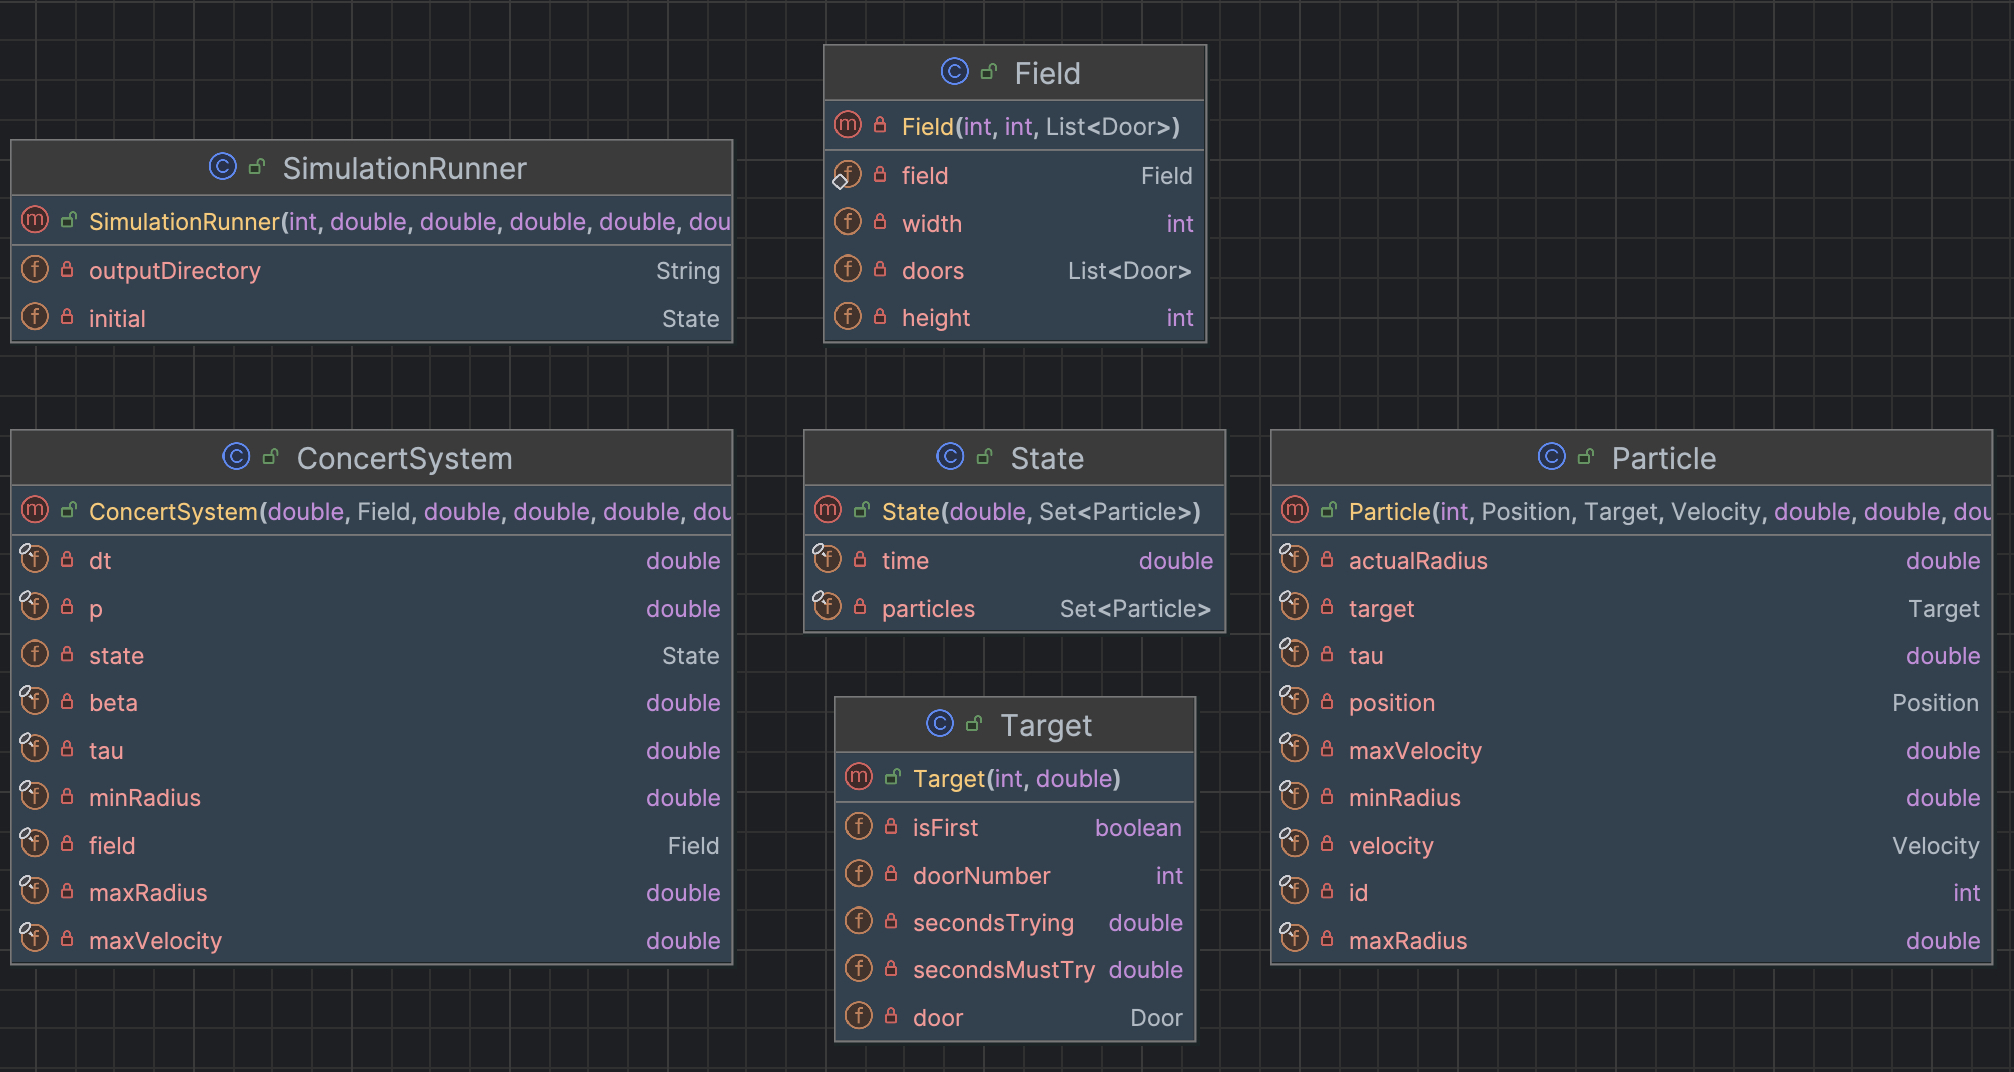
\includegraphics[width=\textwidth]{img/UML.jpg}
    \caption{Diagrama UML del sistema de simulación}
    \label{fig:uml-diagram}
\end{figure}

\subsection{Evolución Temporal}
La evolución del sistema se implementa mediante el método \texttt{next()} que itera sobre todas las partículas:

\begin{algorithm}[H]
\caption{Evolución temporal del sistema}
\begin{algorithmic}[1]
\State $\texttt{newParticles} \leftarrow \emptyset$
\For{$p \in \texttt{state.getParticles()}$}
    \State $\texttt{newParticle} \leftarrow \texttt{escape}(p)$
    \If{$\neg \texttt{hasEscaped}(\texttt{newParticle})$}
        \State $\texttt{newParticles} \leftarrow \texttt{newParticles} \cup \{\texttt{newParticle}\}$
    \EndIf
\EndFor
\State \Return $\texttt{new State}(\texttt{time} + \Delta t, \texttt{newParticles})$
\end{algorithmic}
\end{algorithm}

\subsection{Mecanismo de Escape}
El comportamiento de cada partícula se determina mediante el método \texttt{escape()}, que actualiza su estado según las siguientes reglas:

\begin{algorithm}[H]
\caption{Mecanismo de escape de una partícula}
\begin{algorithmic}[1]
\Function{escape}{$p$}
    \State $\texttt{contacts} \leftarrow \texttt{checkContact}(p)$
    \State $\texttt{newRadius} \leftarrow \texttt{updateRadius}(p, \neg \texttt{contacts.isEmpty()})$
    \State $\texttt{newModule} \leftarrow \texttt{updateModule}(p, \texttt{newRadius})$
    \State $\texttt{newDirection} \leftarrow \texttt{updateDirection}(p, \texttt{contacts})$
    \State $\texttt{newPosition} \leftarrow \texttt{updatePosition}(p, \Delta t)$
    
    \State $p.\texttt{target.step}(\Delta t)$
    \If{$p.\texttt{target.needsChange()}$}
        \State $p.\texttt{target.change}(\texttt{bestNextDoor}(p))$
    \EndIf
    
    \State \Return nueva Partícula$(p.\texttt{id}, \texttt{newPosition}, p.\texttt{target}, \texttt{newDirection}, \texttt{newModule})$
\EndFunction
\end{algorithmic}
\end{algorithm}

\subsection{Selección de Puerta}
La elección de la puerta objetivo se implementa mediante el método \texttt{bestNextDoor()}, que calcula el score para cada puerta según la ecuación ya planteada.

El algoritmo de selección se implementa como:

\begin{algorithm}[H]
\caption{Selección de puerta}
\begin{algorithmic}[1]
\For{cada puerta $d$}
    \State Calcular $RD(d)$ según distancia a la puerta
    \State Calcular $R_\rho(d)$ según densidad local
    \State $S(d) \leftarrow p \times RD(d) + (1-p) \times R_\rho(d)$
\EndFor
\State \Return puerta con máximo $S(d)$
\end{algorithmic}
\end{algorithm}

\subsection{Condición de Escape}
Una partícula se considera que ha escapado cuando su posición coincide con alguna de las puertas de salida, momento en el cual es removida del sistema. El método \texttt{hasEscaped()} verifica esta condición para cada puerta del campo.

\section{Simulaciones}
Se realizaron simulaciones variando dos parámetros principales:

\begin{enumerate}
    \item Factor $p$: influye en el balance entre elegir la puerta más cercana o la de menor densidad
    \item Tiempo de re-decisión $ct$: intervalo en el que cada partícula reevalúa su elección de puerta
\end{enumerate}

Para cada combinación de parámetros se realizaron 15 realizaciones independientes con:
\begin{itemize}
    \item $r_{\text{min}} = 0.15\text{ m}$
    \item $r_{\text{max}} = 0.35\text{ m}$
    \item $v_{\text{max}} = 1.0\text{ m/s}$
    \item $\beta = 0.9$
    \item $\tau = 0.5\text{ s}$
    \item 500 agentes
\end{itemize}

\section{Observables}

\subsection{Tiempo de Evacuación}
Se mide el tiempo total hasta que todas las partículas evacúan el recinto.

\subsection{Caudal}
El caudal total se calcula como:
\begin{equation}
Q(t) = N(t) - N(t + \Delta t)
\end{equation}

donde:
\begin{itemize}
    \item $Q(t)$ es el caudal en el tiempo $t$
    \item $N(t)$ es el número total de partículas en el tiempo $t$
    \item $\Delta t$ es el intervalo de tiempo fijo (1 segundo)
\end{itemize}

Se analizan dos métricas:
\begin{enumerate}
    \item $Q_{global}$: número total de agentes por puerta / tiempo total
    \item Interpolación lineal de las curvas de descarga $N(t)$
\end{enumerate}

\subsection{Densidad Media}
La densidad media se calcula como:
\begin{equation}
\rho(t) = \frac{1}{N} \sum_{i=1}^{N} \frac{n_i(t)}{A_c}
\end{equation}

donde:
\begin{itemize}
    \item $N$ es el número total de circunferencias
    \item $n_i(t)$ es el número de partículas en la circunferencia $i$ en tiempo $t$
    \item $A_c$ es el área de cada (semi) circunferencia
\end{itemize}
Tener en cuenta que, como ya dicho anteriormente, se considera para las circunferencias un radio hasta la $k=5$ partícula mas cercana respecto del centro de la circunferencia.

\subsection{Coeficiente de Uniformidad}

Para analizar la distribución de la evacuación entre las diferentes salidas, definimos un coeficiente de uniformidad que nos permite cuantificar qué tan equitativamente se utilizan las puertas disponibles. 

Sea $N$ el número total de puertas de salida y $t$ el tiempo de simulación. Para cada puerta $i$, definimos:
\[
n_i(t) = \text{número de partículas que han salido por la puerta } i \text{ hasta el tiempo } t
\]

\[
\Delta n_i(t) = n_i(t + \Delta t) - n_i(t) = \text{número de partículas que salen por la puerta } i \text{ durante } [t, t+\Delta t]
\]

Para analizar la uniformidad de la evacuación, dividimos el tiempo total en ventanas temporales de tamaño $\Delta t$. En cada ventana temporal $[t, t+\Delta t]$, calculamos la media $\mu(t)$ y la desviación estándar $\sigma(t)$ del número de partículas que salen por cada puerta.

El coeficiente de uniformidad se define entonces como:
\[
U(t) = 1 - \frac{\sigma(t)}{\mu(t)}
\]


\section{Resultados}

\subsection{Estados de las animaciones}

A continuación se muestran frames de aniamciones características del sistema, en donde se varía el parámetro de ponderación $p$.
\begin{figure}[H]
\centering
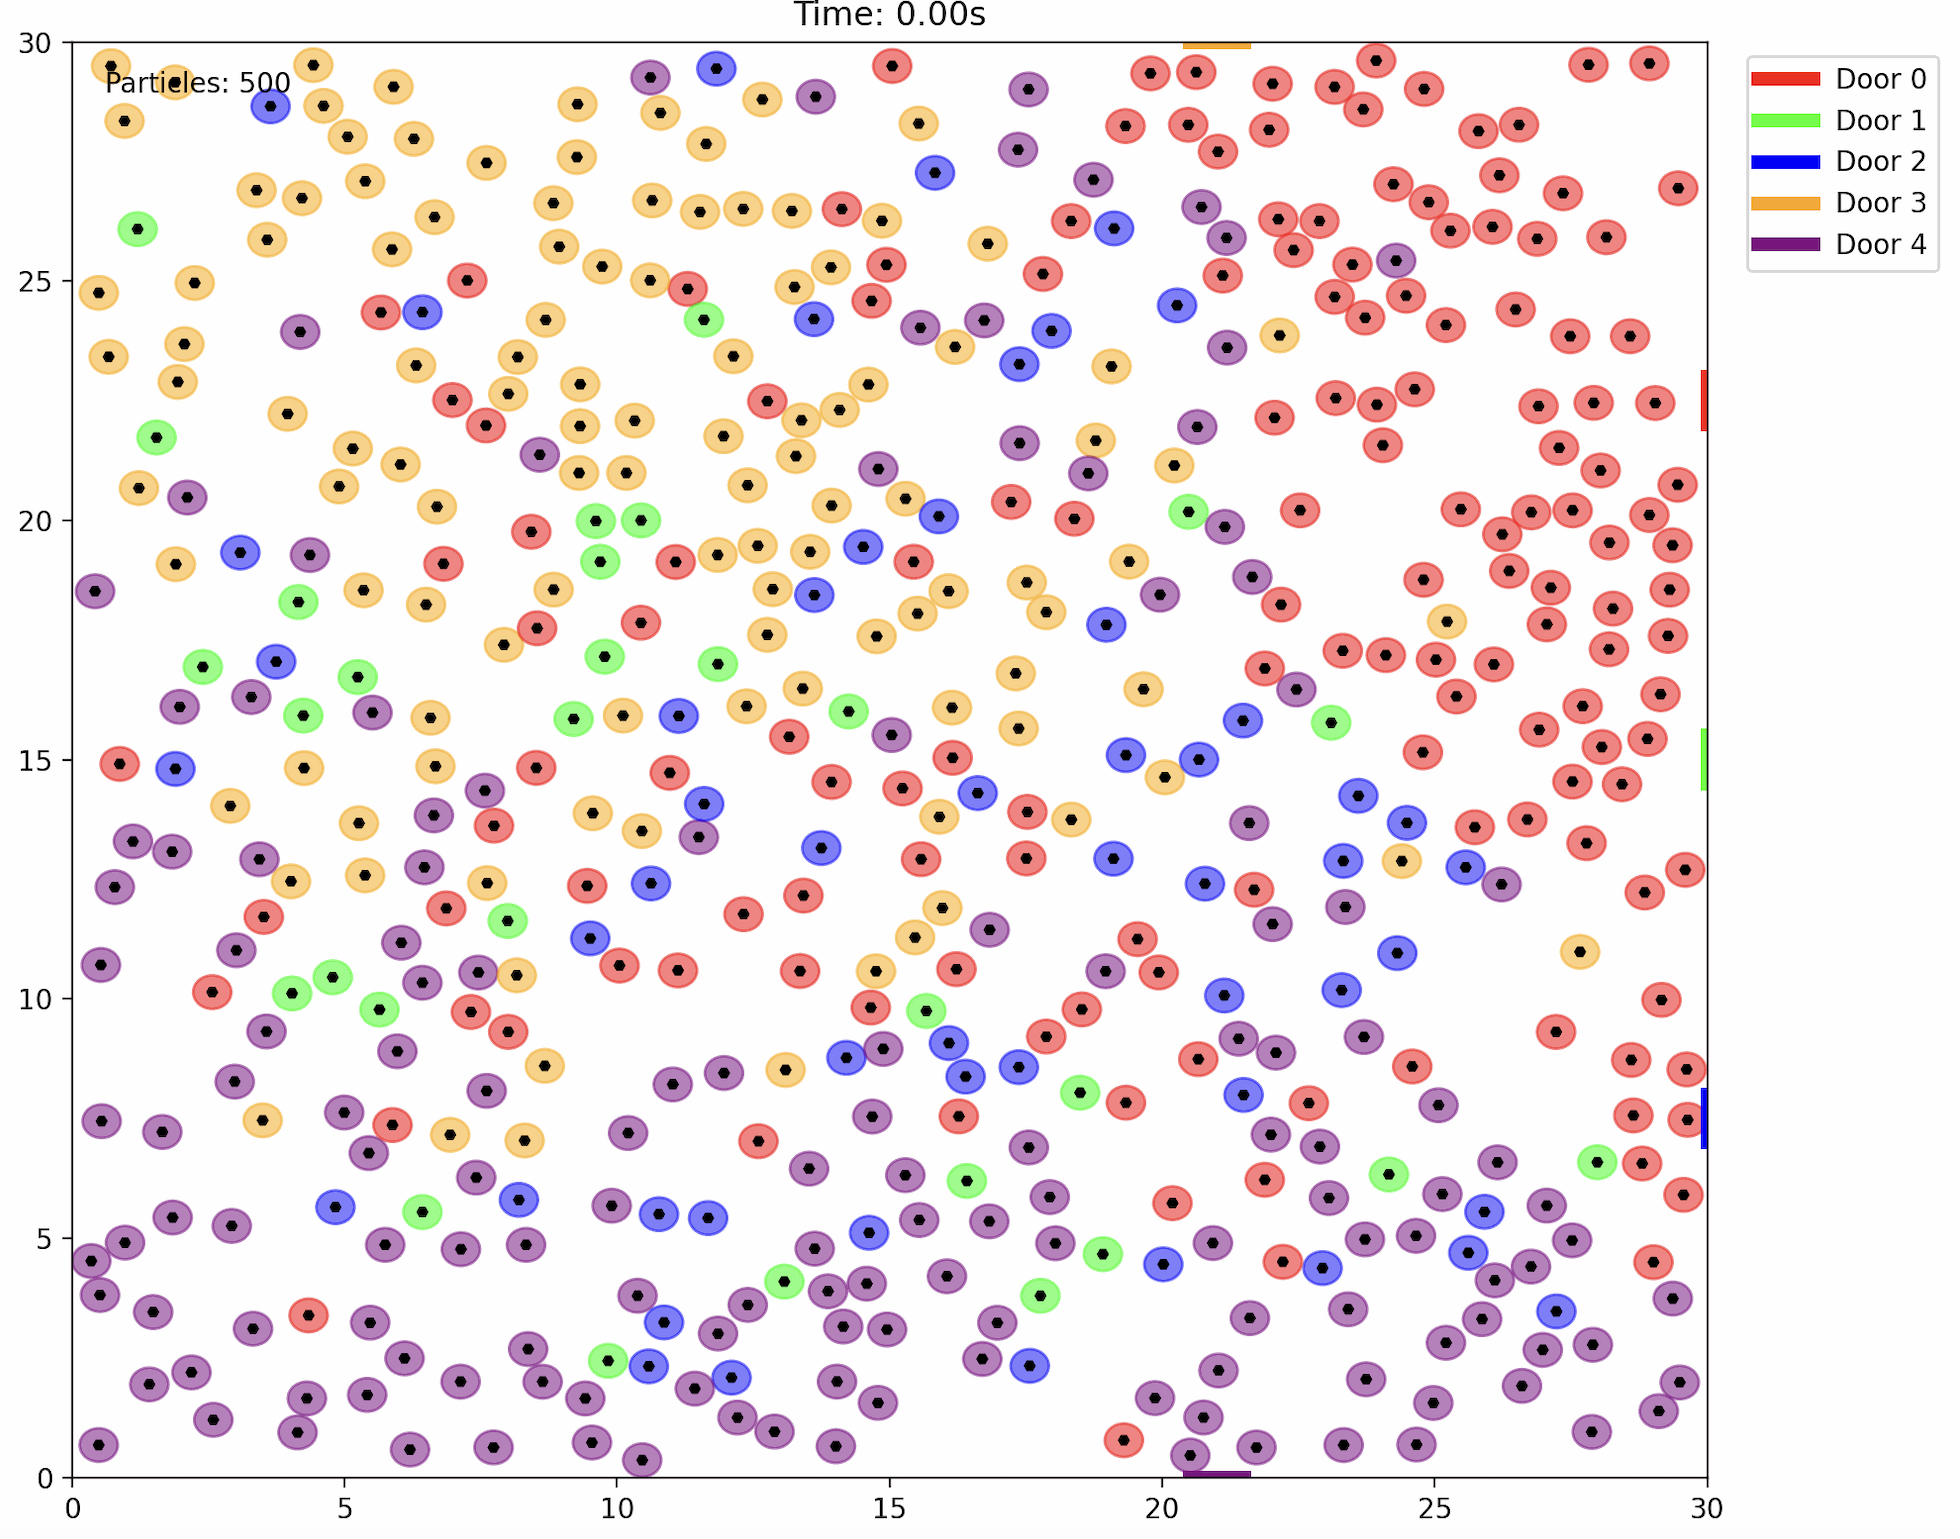
\includegraphics[width=0.9\textwidth]{img/frames/t_20_&_p_0.00.jpg}
\caption{Estado inicial para $p=0.00$}
\label{fig:evac_time_ct}
\end{figure}

\begin{figure}[H]
\centering
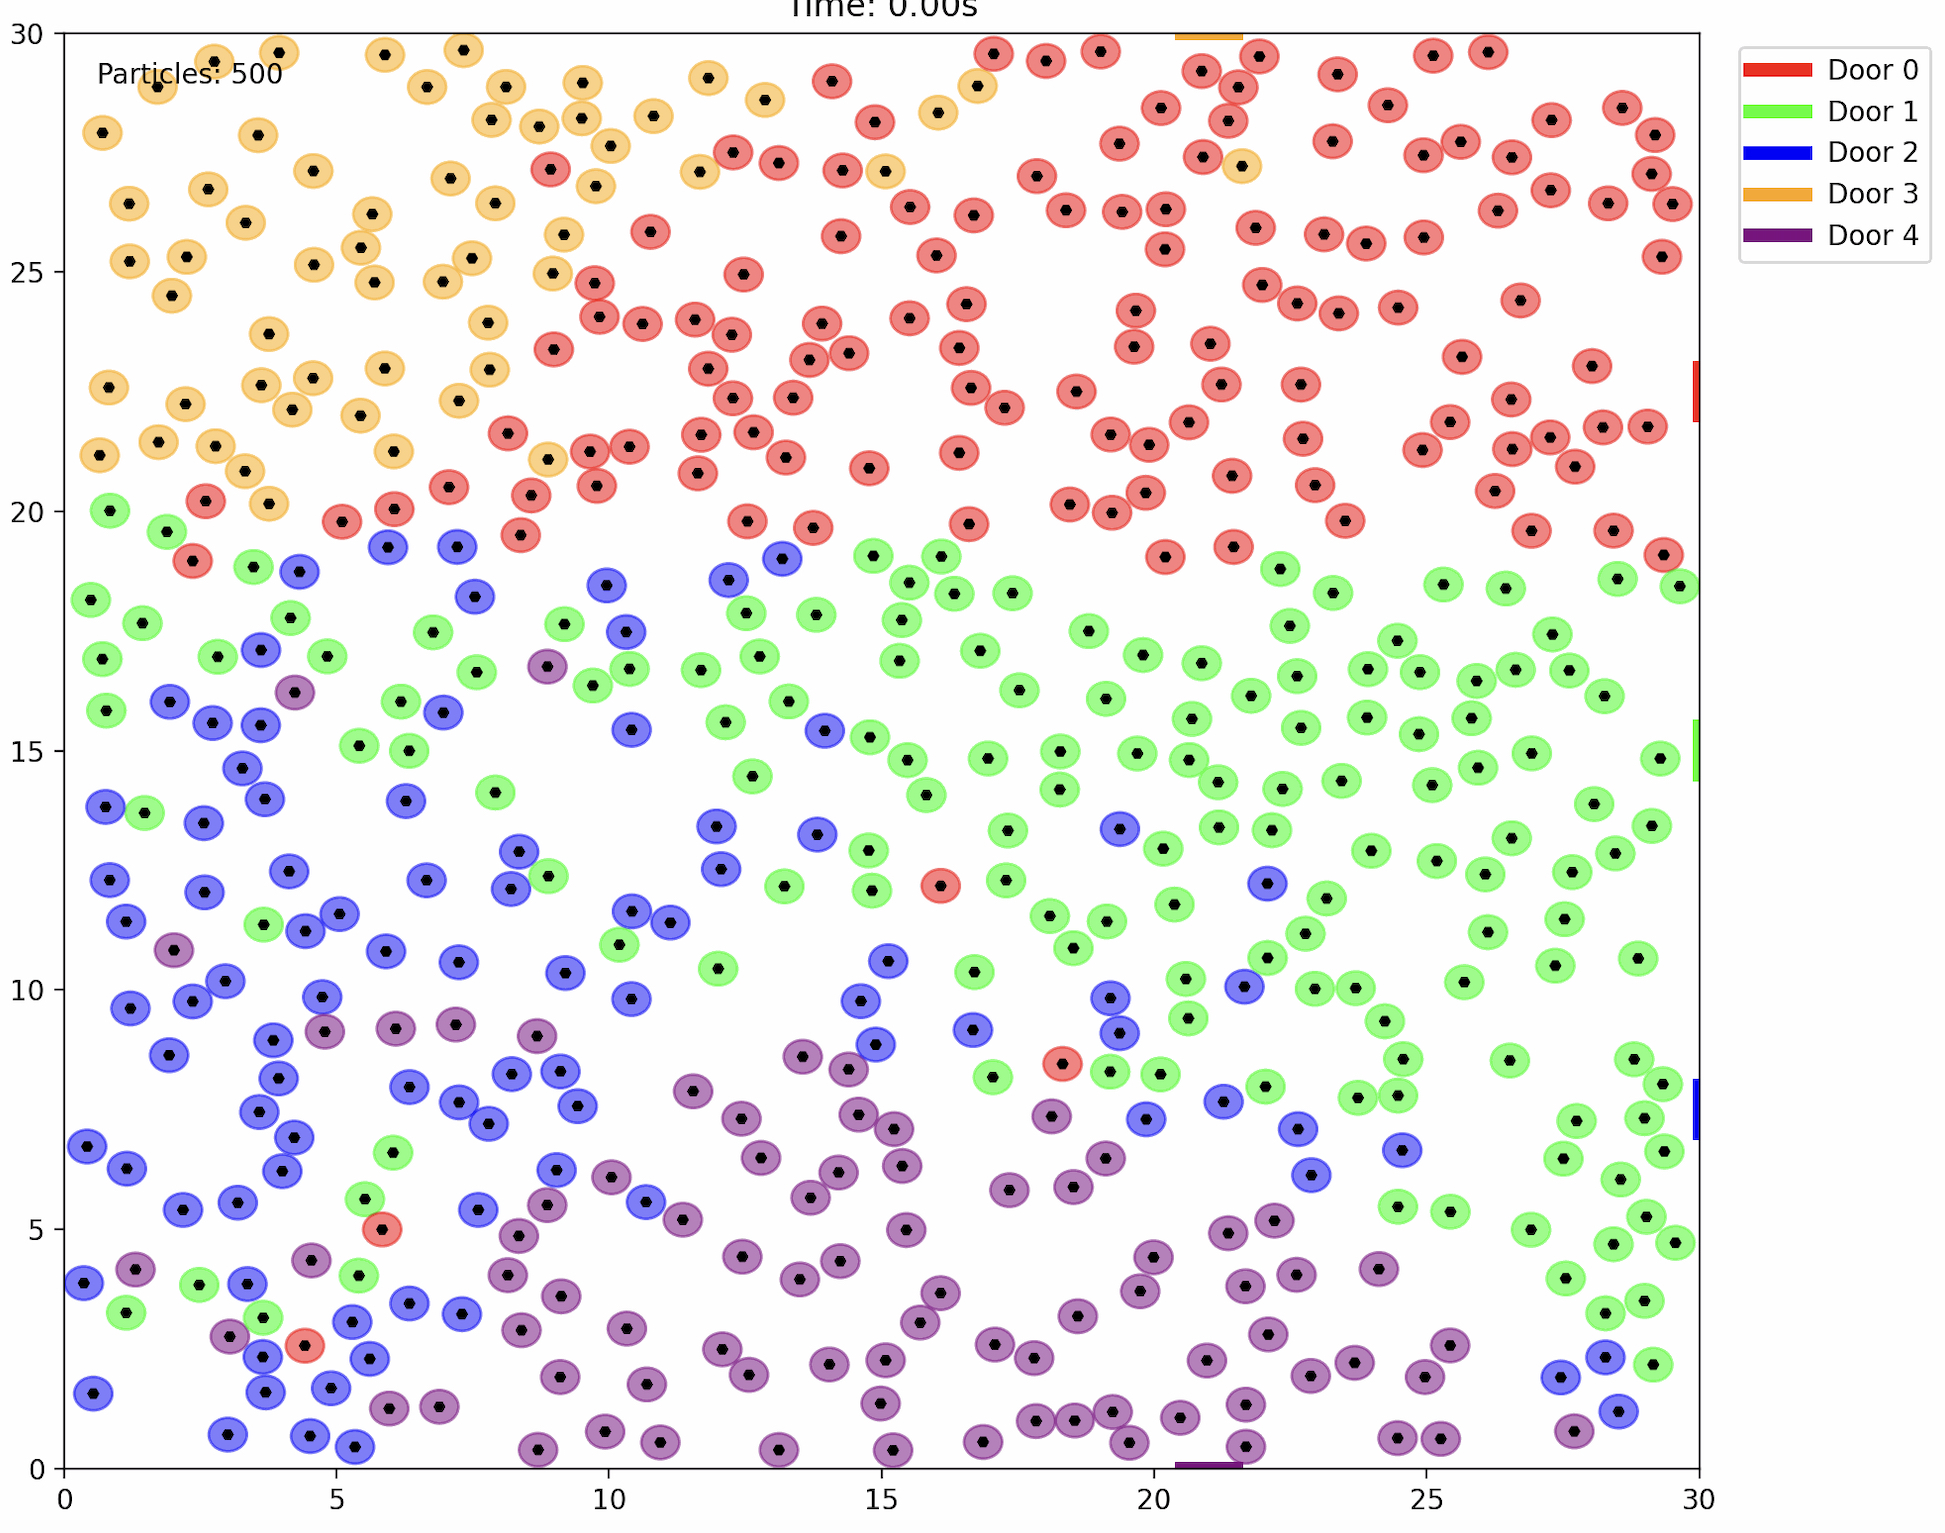
\includegraphics[width=0.9\textwidth]{img/frames/t_20_&_p_0.50.jpg}
\caption{Estado inicial para $p=0.50$}
\label{fig:evac_time_ct}
\end{figure}

\begin{figure}[H]
\centering
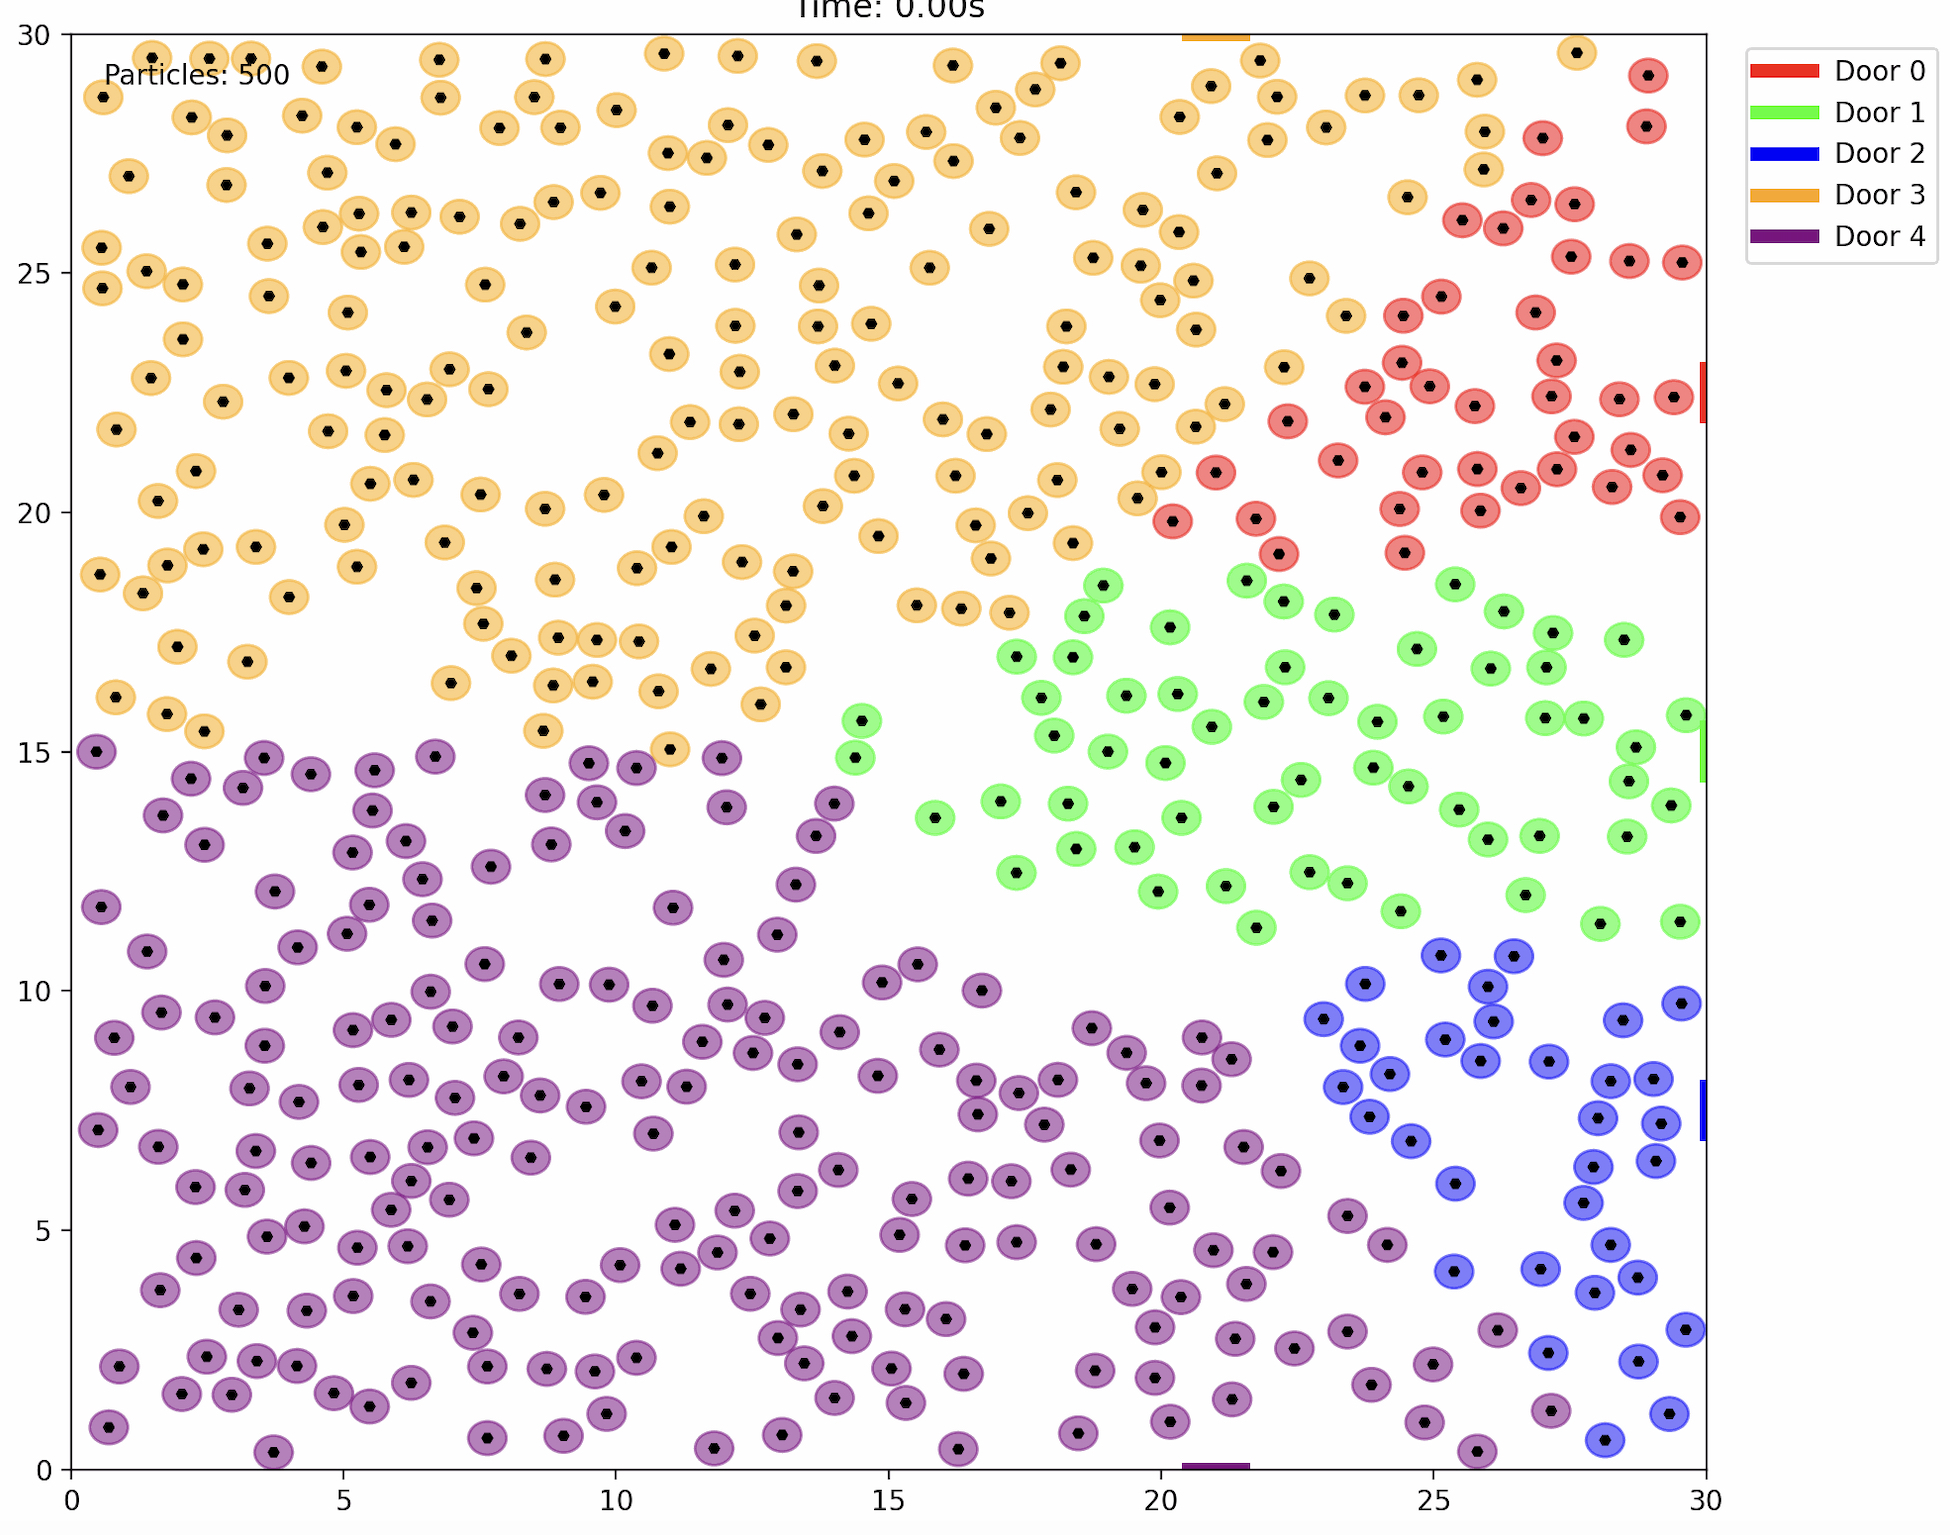
\includegraphics[width=0.9\textwidth]{img/frames/t_20_&_p_1.00.jpg}
\caption{Estado inicial para $p=1.00$}
\label{fig:evac_time_ct}
\end{figure}
Se puede notar que a medida que $p$ se acerca a 1, las partículas están mas agrupadas y mantienen su elección por la puerta más cercana, sin perder tiempo en ir cambiando de puerta en función de la densidad que hay en las mismas.

\subsection{Análisis del Tiempo de Evacuación en función del parámetro de ponderación ($p$), para $ct=45$}
\begin{figure}[H]
\centering
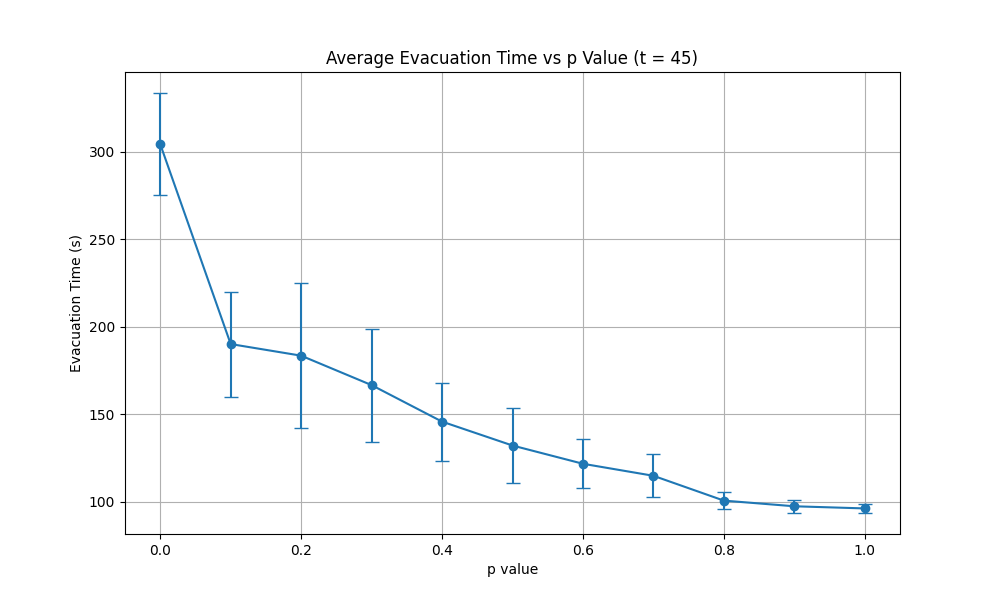
\includegraphics[width=0.9\textwidth]{img/evacuation_times_t_45.png}
\caption{Tiempo promedio de evacuación en función del parámetro de ponderación ($p$) para $ct=45$}
\label{fig:evac_time_ct}
\end{figure}
En cuanto al impacto que tiene el parámetro de ponderación, que define que métrica tiene más importancia a la hora de elegir la puerta óptima, tomando valores cercanos a 0 a medida que la densidad en cada puerta se vuelve más importante y valores cercanos a 1 cuanto más relevante es la distancia entre la partícula y la puerta, se puede notar que a medida que la distancia se torna más importante en la elección el tiempo que tardan en evacuar las partículas es menor. Esto se debe a que como la distancia en un criterio fijo ya que las puertas no se mueven, desde un principio las partículas no tienden a cambiar mucho su elección inicial, por lo que no pierden tiempo trasladándose de una puerta hacia otra.

\subsection{Análisis del Flujo Acumulado de Evacuación}
Los gráficos de flujo acumulado por puerta revelan patrones distintivos según el valor del parámetro $p$, manteniendo constante el tiempo de re-decisión ($ct=20s$):

\subsubsection{Caso $p=1.00$: Priorizando la Distancia}

\begin{figure}[H]
    \centering
    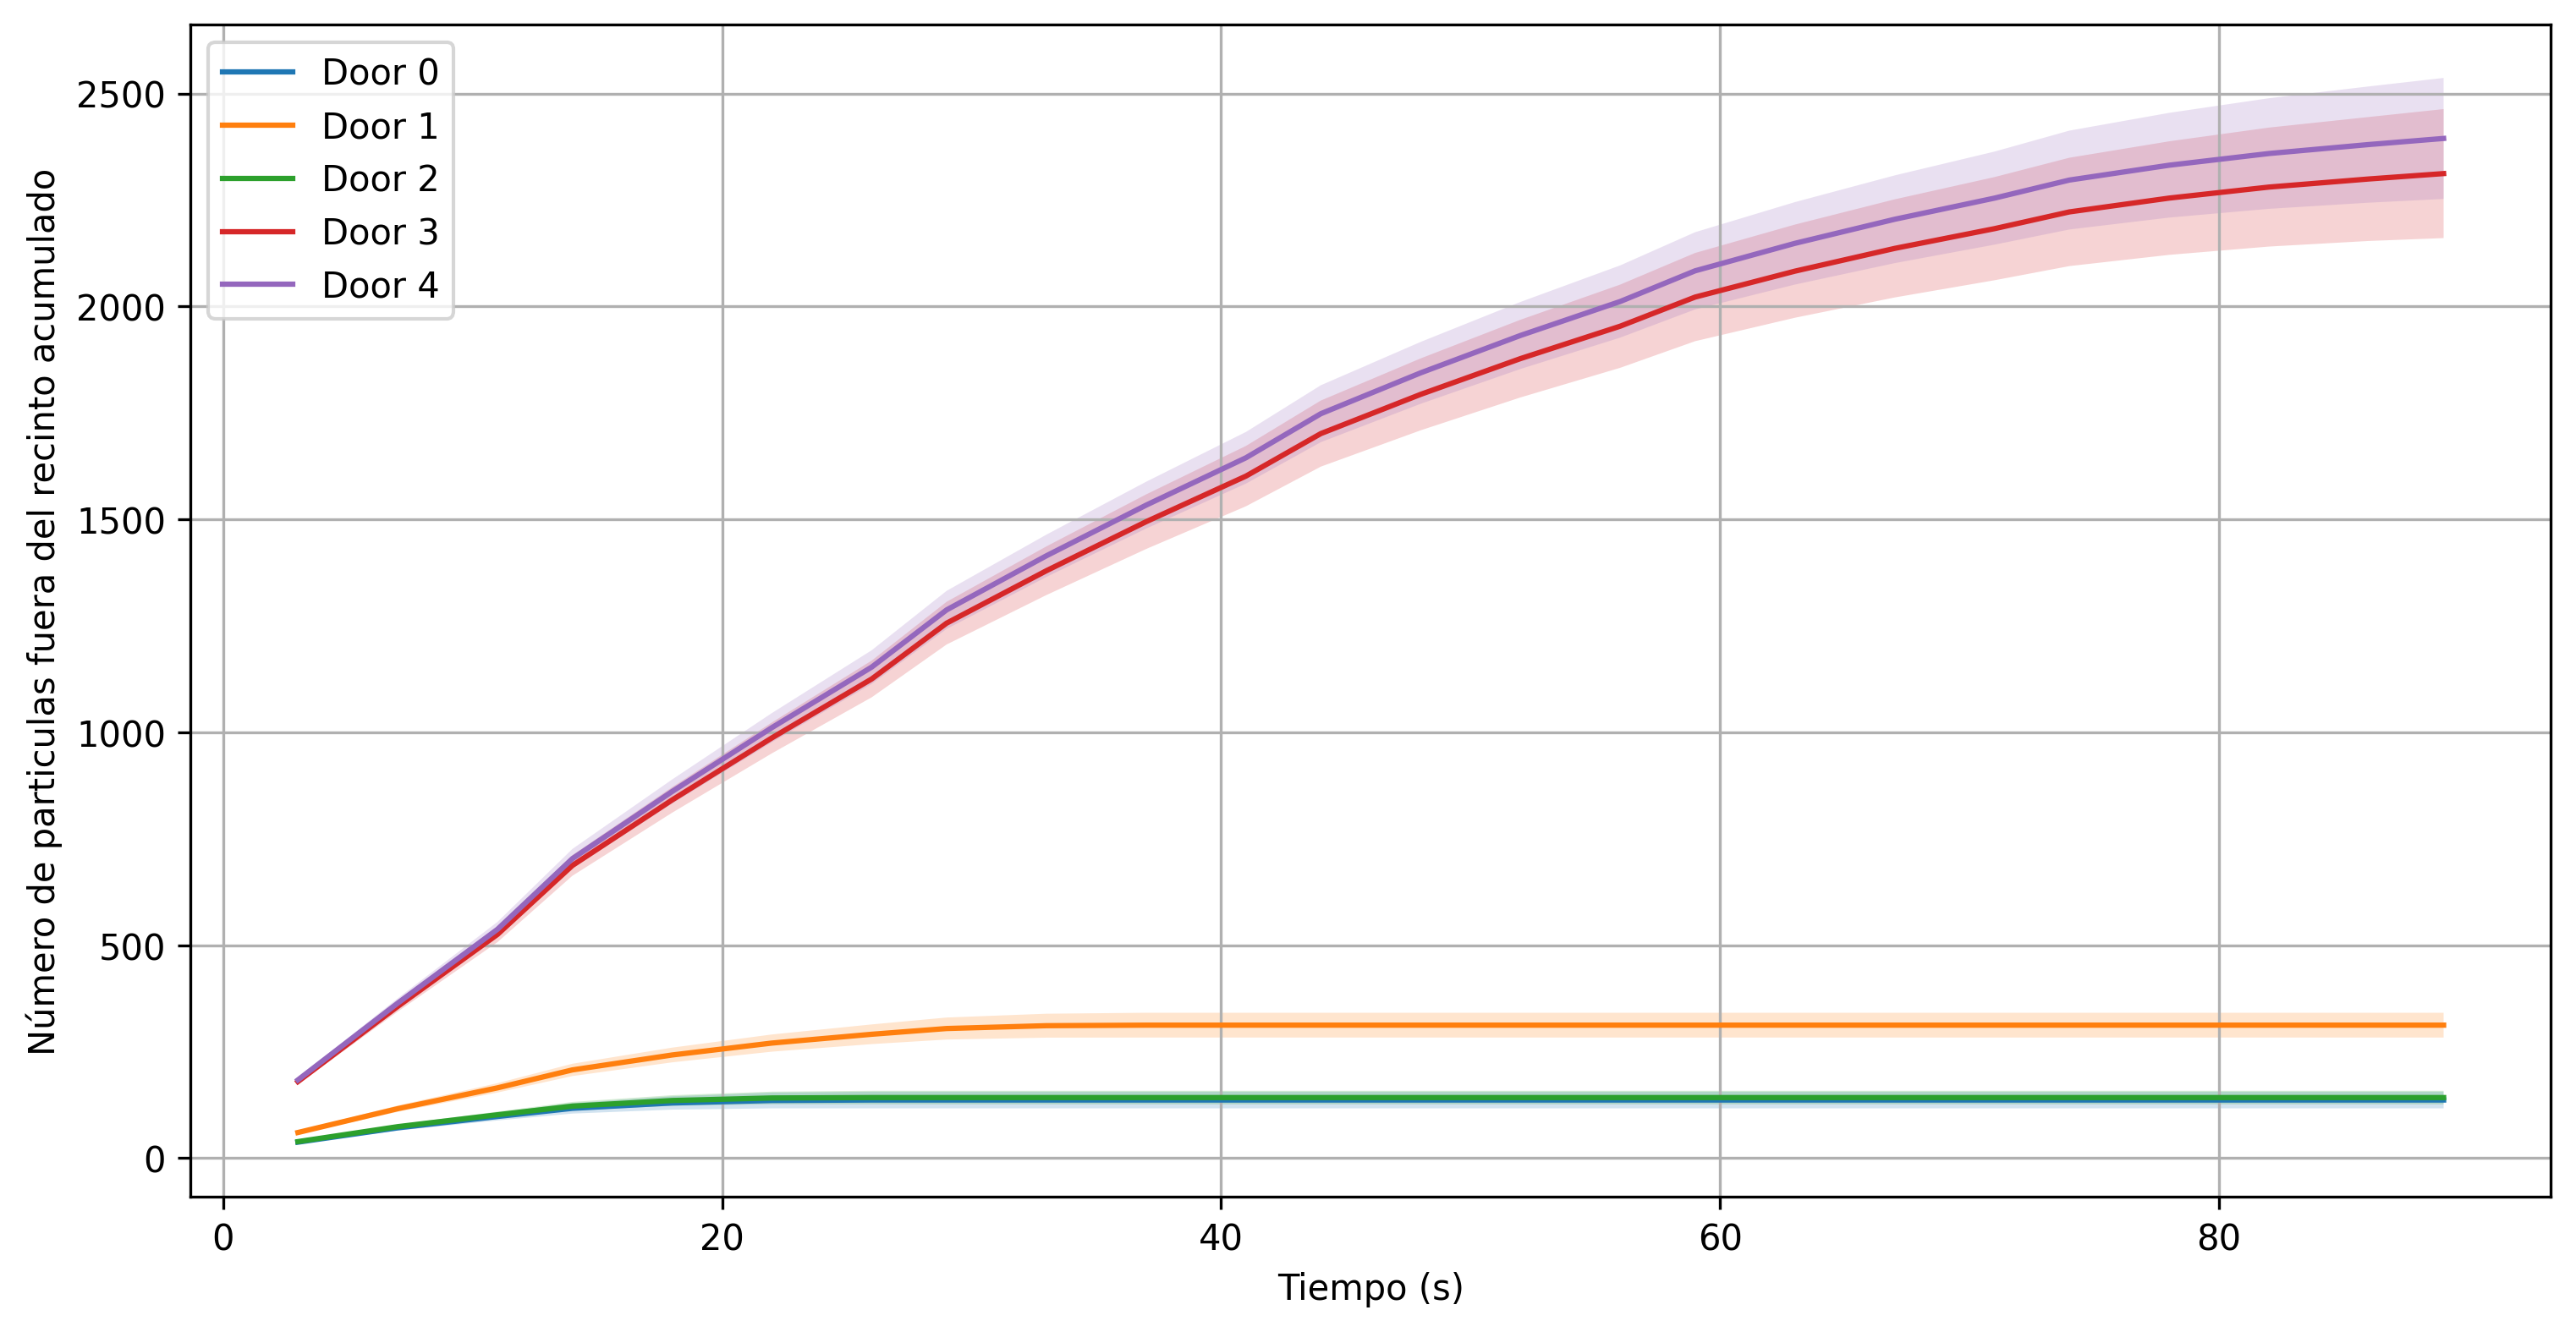
\includegraphics[width=0.9\textwidth]{img/cumulative_door_flows_t_20_&_p_1.00.png}
    \caption{Flujo acumulado de evacuación para $p=1.00$}
    \label{fig:flow_p100}
\end{figure}

El flujo acumulado muestra una marcada preferencia por las puertas 3 y 4, que acumulan aproximadamente el 80\% de las evacuaciones (cerca de 2300 partículas). Las puertas 1 y 2 muestran un flujo significativamente menor, alcanzando apenas 300 partículas cada una. Esta distribución desigual resulta en un tiempo de evacuación relativamente corto (80 segundos) pero evidencia una utilización ineficiente de las salidas disponibles.

\subsubsection{Caso $p=0.50$: Balance entre Distancia y Densidad}

\begin{figure}[H]
    \centering
    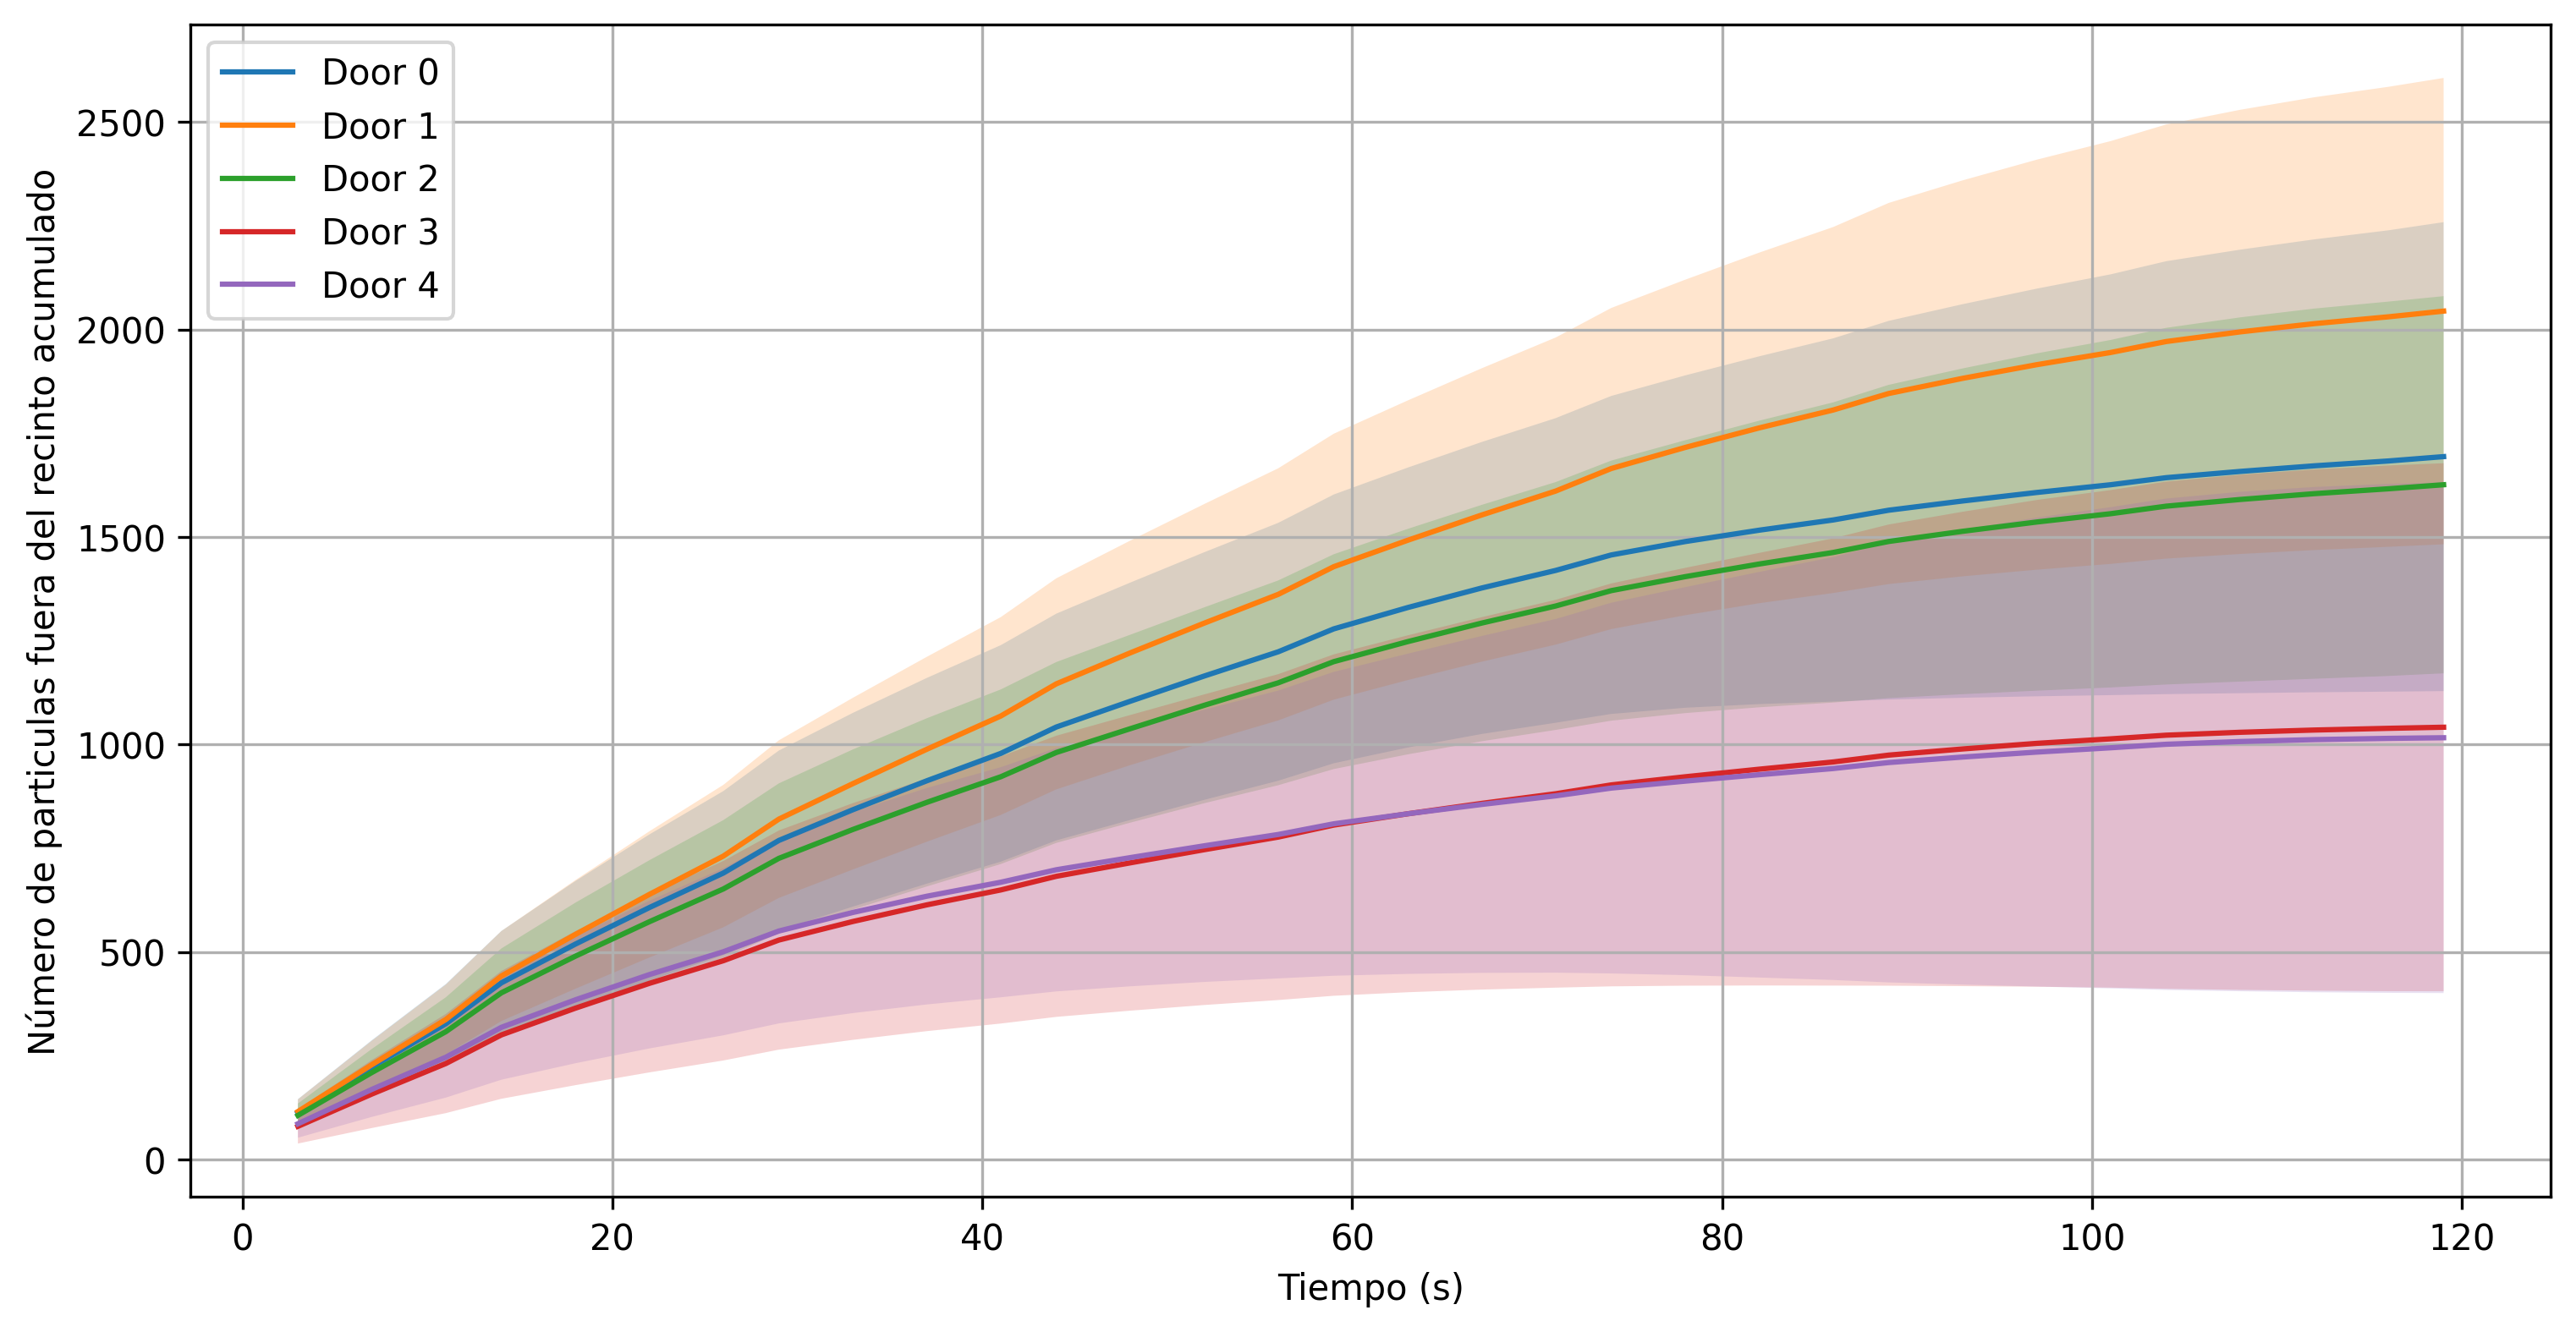
\includegraphics[width=0.9\textwidth]{img/cumulative_door_flows_t_20_&_p_0.50.png}
    \caption{Flujo acumulado de evacuación para $p=0.50$}
    \label{fig:flow_p050}
\end{figure}

Con un equilibrio entre los factores de decisión, se observa una distribución más uniforme del flujo entre las puertas. Las curvas muestran pendientes similares, indicando tasas de evacuación más homogéneas. El tiempo total de evacuación aumenta a 120 segundos, pero la varianza entre los flujos de las diferentes puertas se reduce significativamente. Las puertas 0, 1 y 2 muestran flujos acumulados similares (aproximadamente 1600-2000 partículas), mientras que las puertas 3 y 4 mantienen flujos levemente menores (1000 partículas).

\subsubsection{Caso $p=0.00$: Priorizando la Densidad}

\begin{figure}[H]
    \centering
    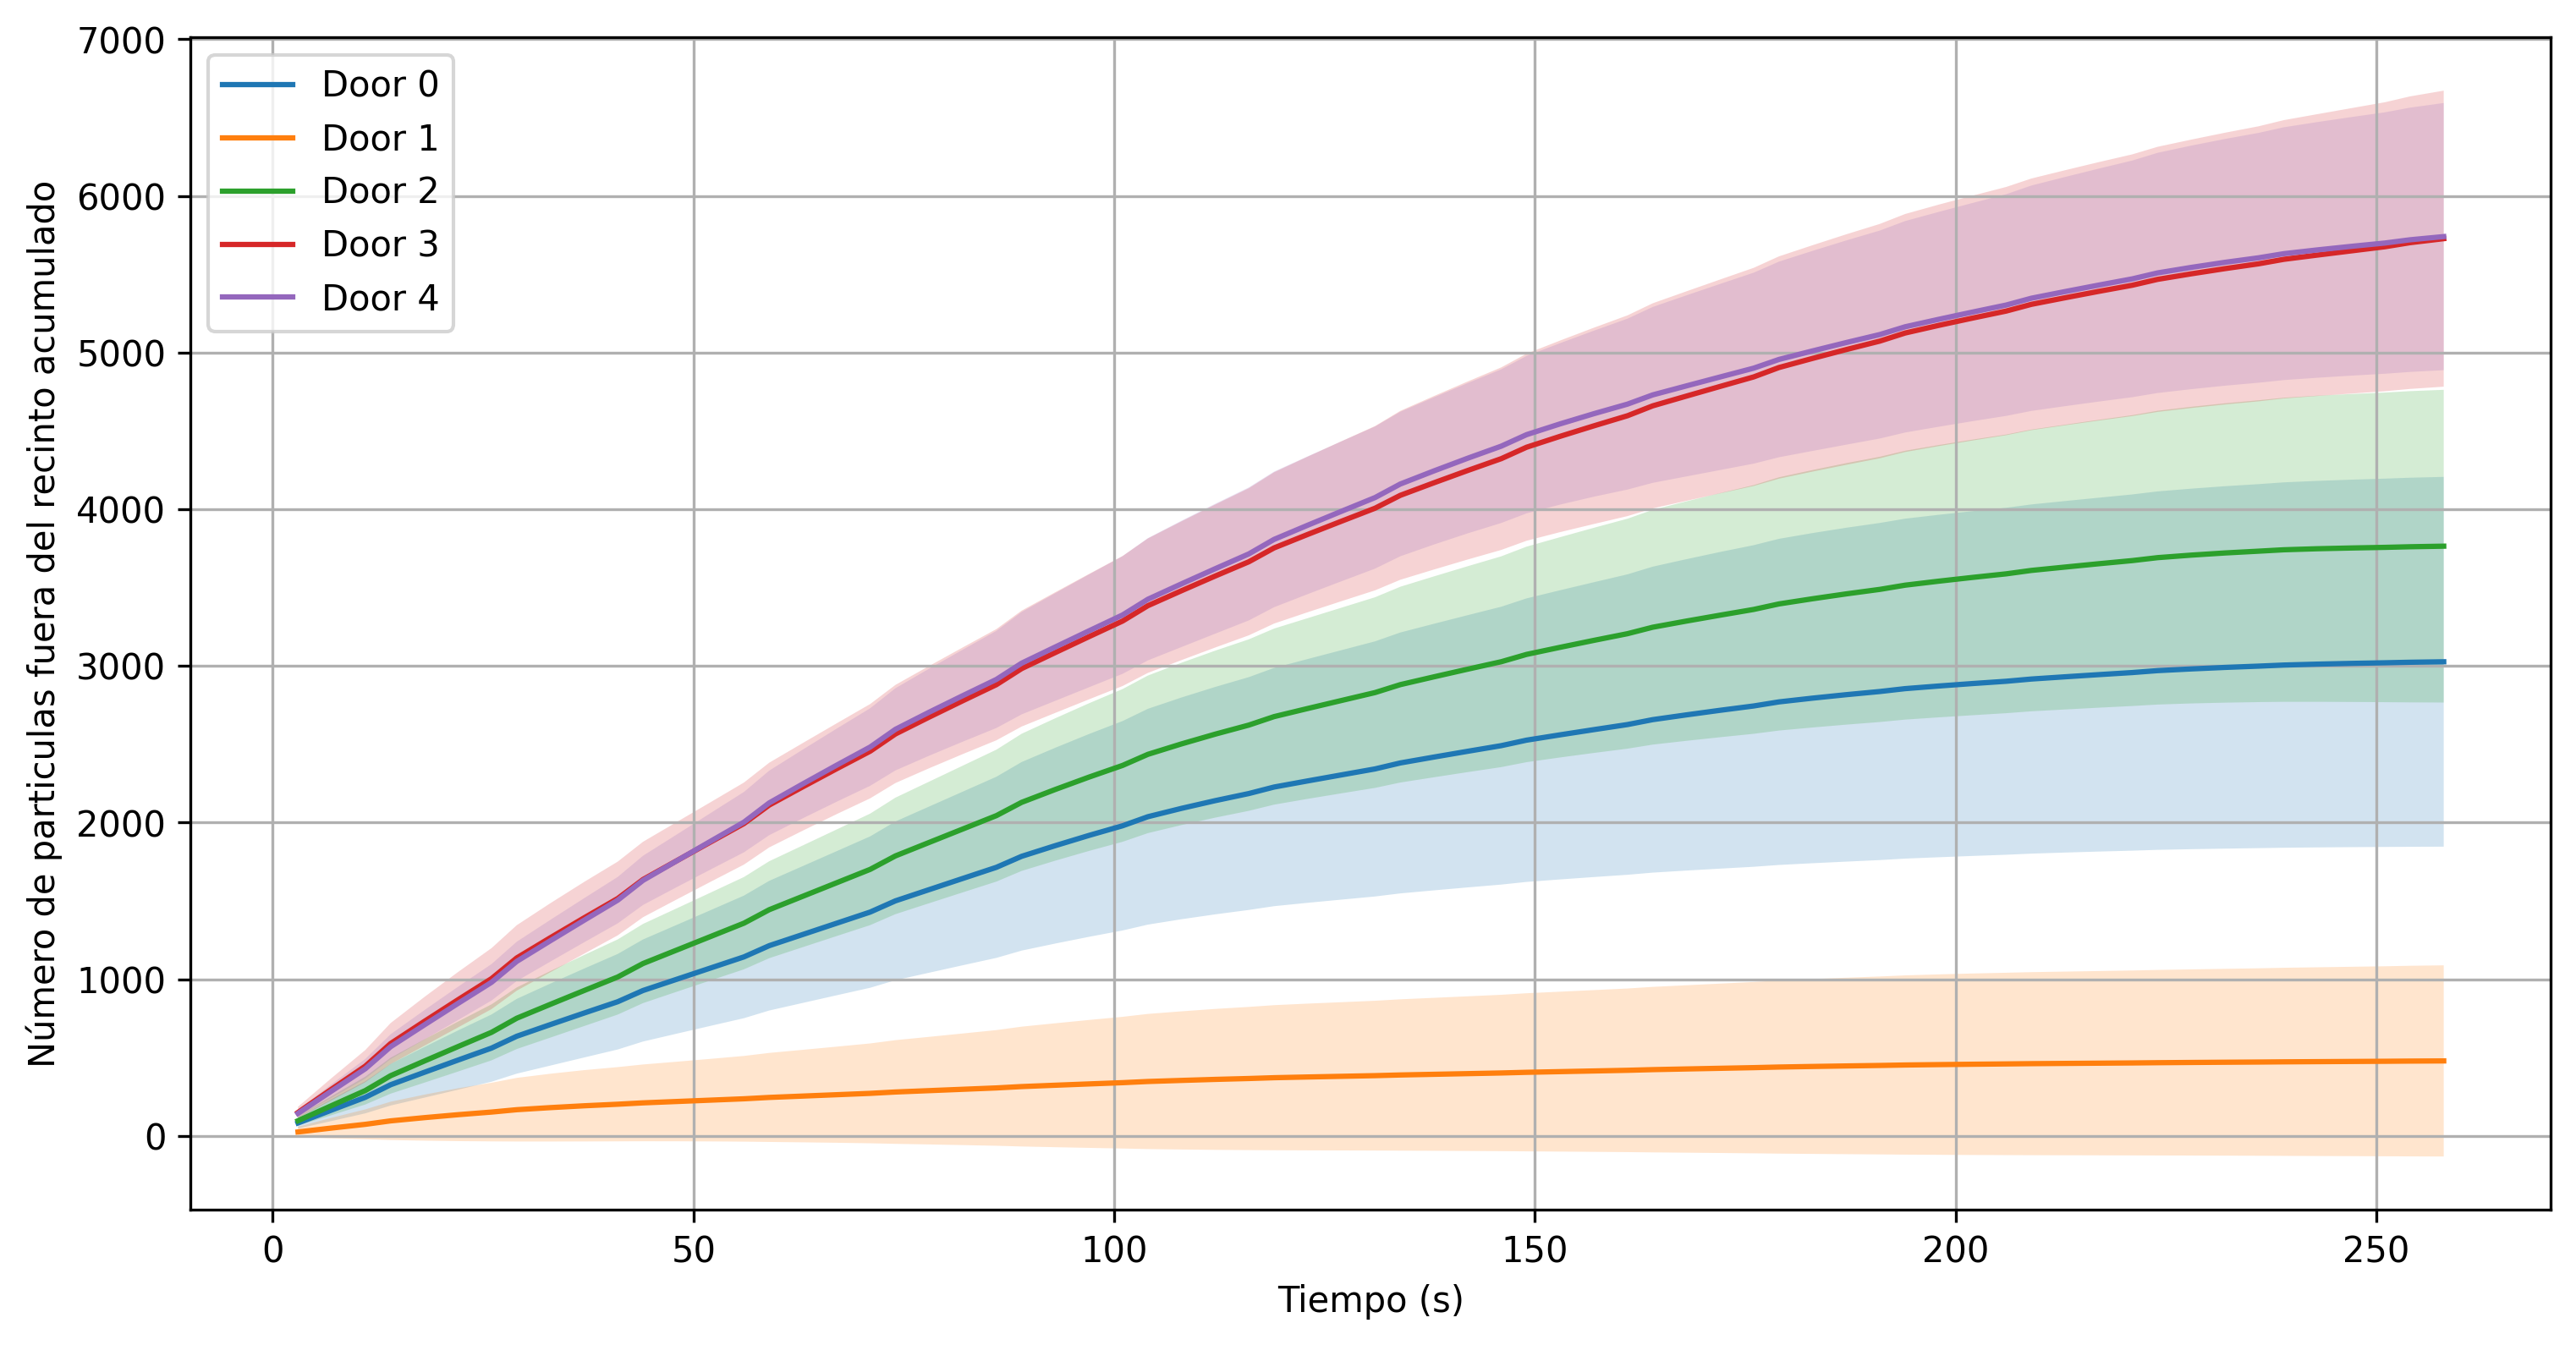
\includegraphics[width=0.9\textwidth]{img/cumulative_door_flows_t_20_&_p_0.00.png}
    \caption{Flujo acumulado de evacuación para $p=0.00$}
    \label{fig:flow_p000}
\end{figure}

La consideración exclusiva de la densidad resulta en el tiempo de evacuación más largo (250 segundos) pero muestra una distribución más equitativa del flujo entre las puertas 2, 3 y 4 (aproximadamente 3000-5500 partículas cada una). 

Este análisis revela que mientras la priorización de la distancia ($p=1.00$) resulta en evacuaciones más rápidas pero congestionadas, la consideración de la densidad ($p=0.00$) produce evacuaciones más lentas pero con una distribución más equilibrada del flujo. El caso intermedio ($p=0.50$) representa un compromiso razonable entre estos extremos, sugiriendo que una estrategia mixta podría ser óptima en situaciones reales de evacuación.

\subsection{Análisis del Caudal de Partículas}

Se analizó el flujo de partículas (caudal) para diferentes valores del parámetro $p$ manteniendo constante el tiempo de re-decisión ($ct=20s$). Los resultados muestran patrones característicos para cada configuración:

\subsubsection{Caudal en función de $p$}

\begin{figure}[H]
    \centering
    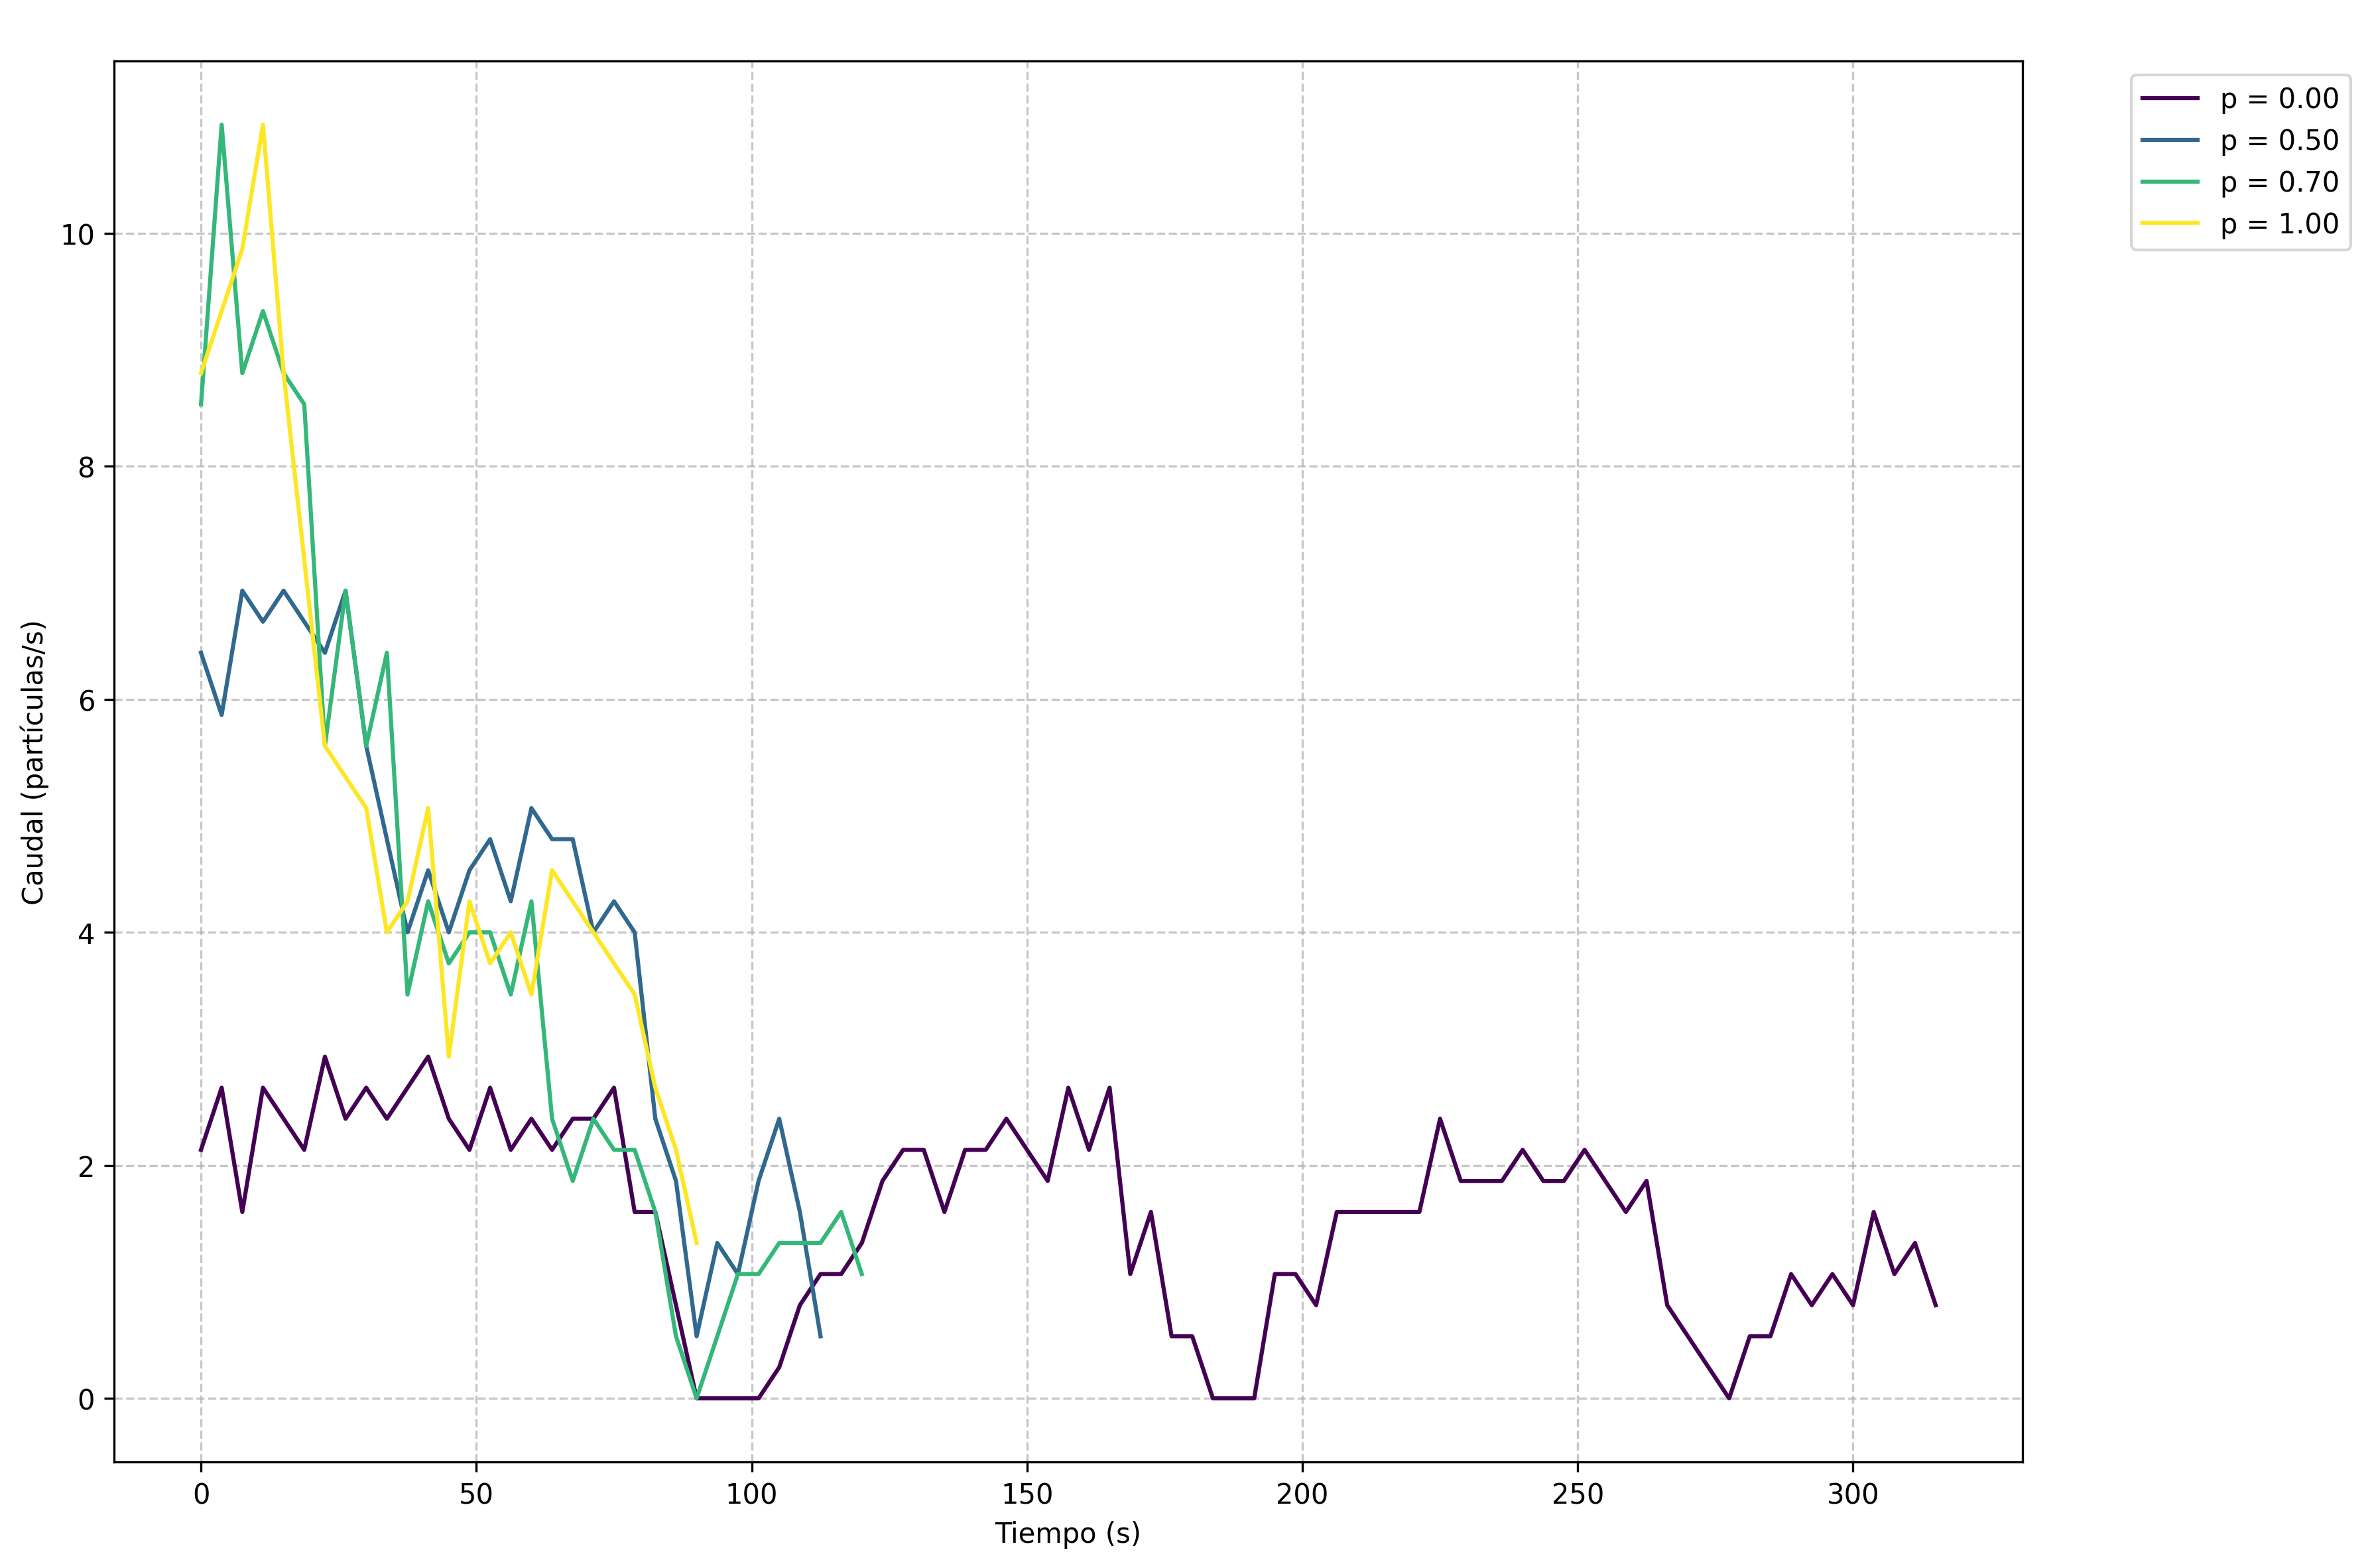
\includegraphics[width=0.9\textwidth]{img/caudal_vs_time_t45.png}
    \caption{Caudal global en función del tiempo para $ct=45$}
    \label{fig:flow_p100}
\end{figure}
Se puede observar que a medida que la densidad es menor decisiva, el caudal global es mayor. Esto se debe a que las partículas ya desde el comienzo tienen una fuerte preferencia por la puerta más cercana y siempre la siguen eligiendo sin importar la densidad que haya en la misma, lo que provoca un gran caudal en algunas puertas, mientras que en otras el caudal es más pequeño o nulo.

\subsubsection{Caudal para $p = 1.00$}
Caso donde los agentes priorizan totalmente la distancia.

\begin{figure}[H]
    \centering
    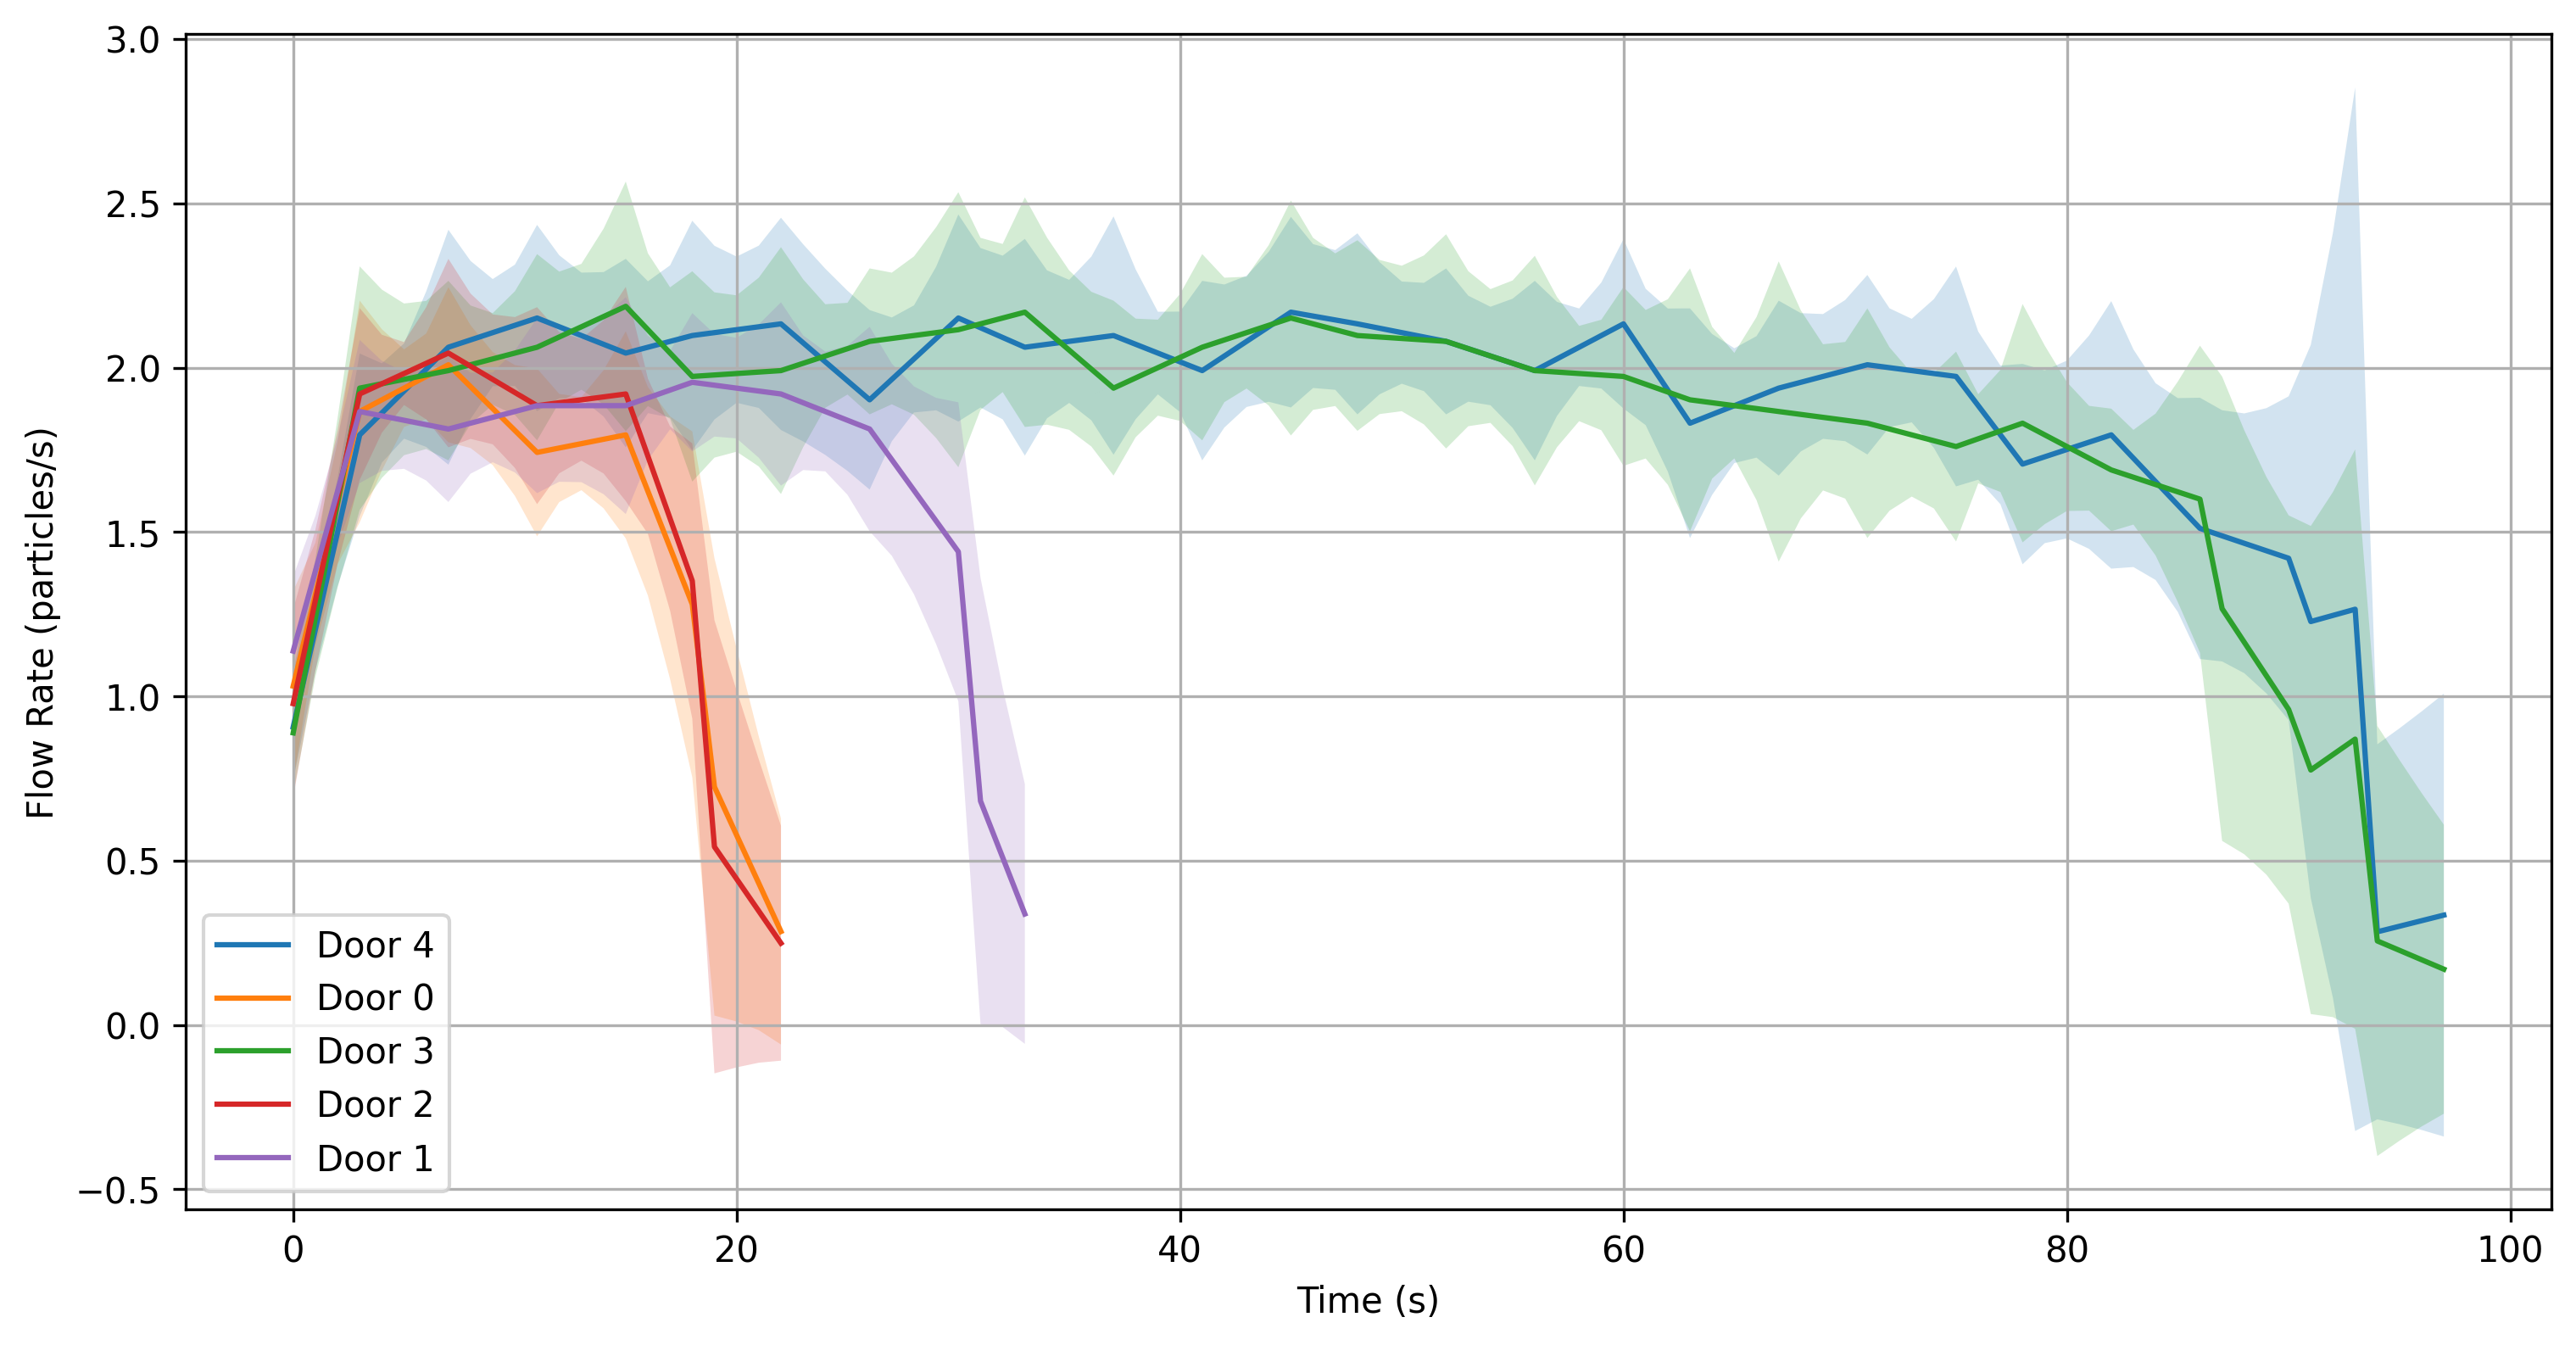
\includegraphics[width=0.9\textwidth]{img/door_flow_rates_t_20_&_p_1.00.png}
    \caption{Caudal promedio de partículas para $p=1.00$}
    \label{fig:caudal_p100}
\end{figure}

\subsubsection{Caudal para $p = 0.50$}
Con un balance entre distancia y densidad ($p = 0.50$), se observa:

\begin{figure}[H]
    \centering
    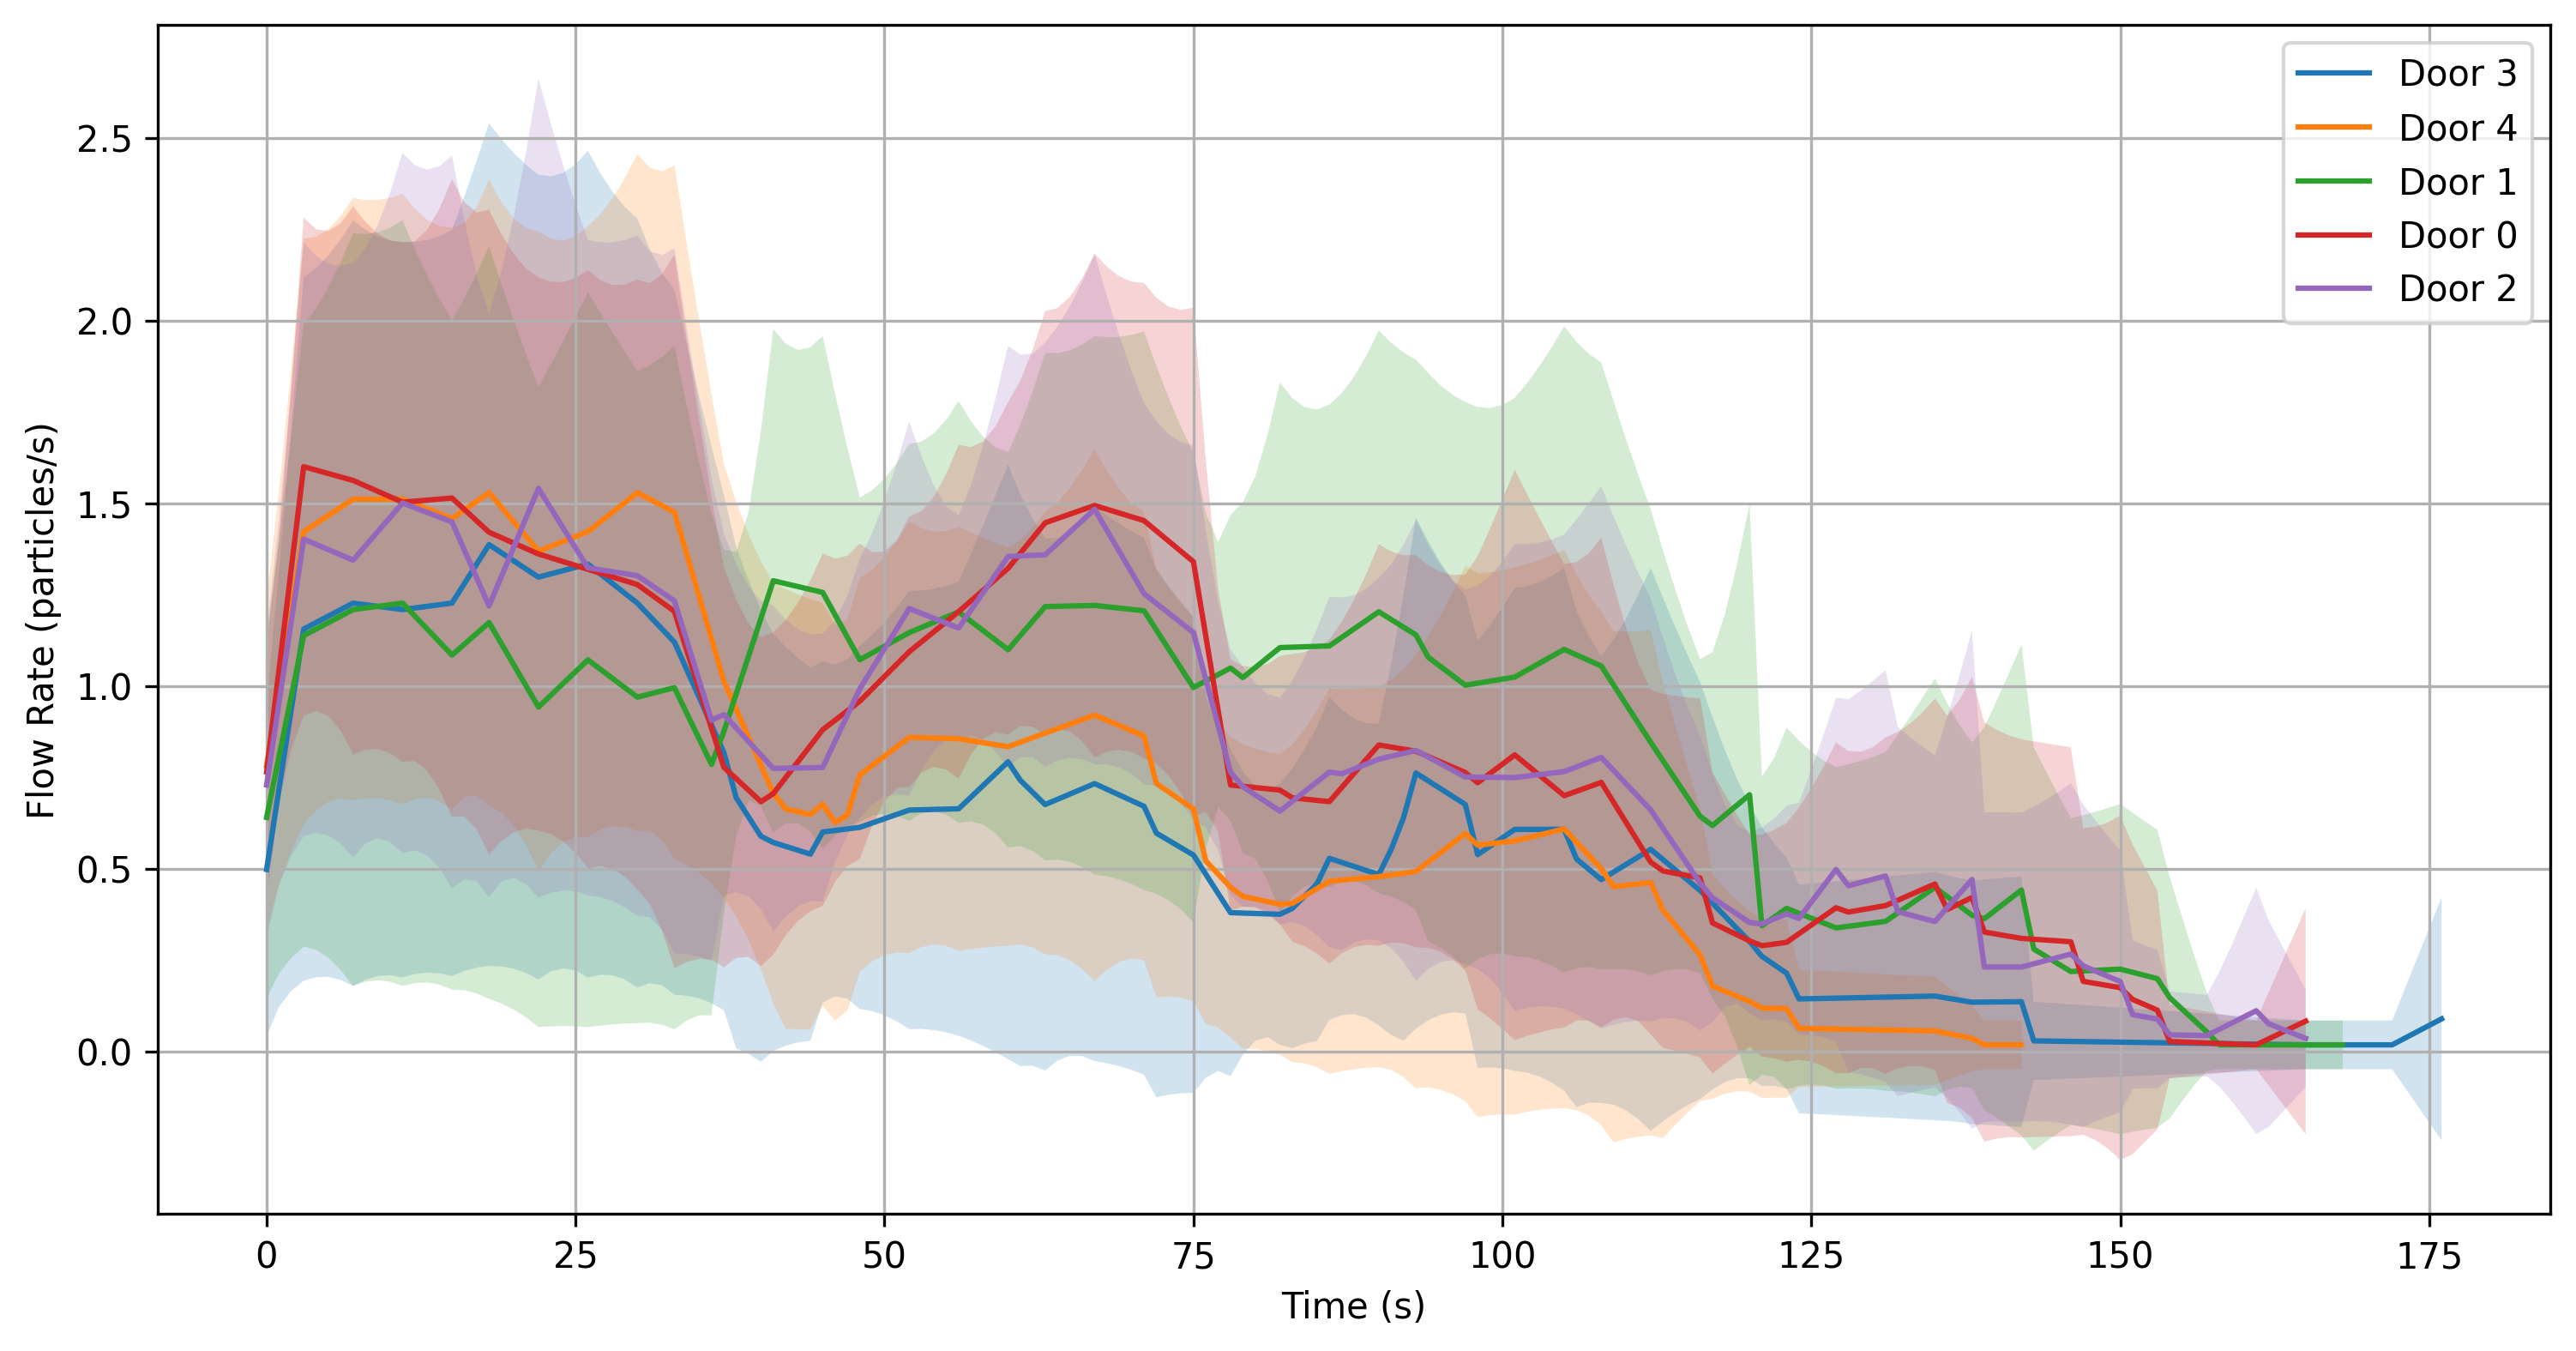
\includegraphics[width=0.9\textwidth]{img/door_flow_rates_t_20_&_p_0.50.png}
    \caption{Caudal promedio de partículas para $p=0.50$}
    \label{fig:caudal_p050}
\end{figure}

\subsubsection{Caudal para $p = 0.00$}
Cuando los agentes priorizan exclusivamente la densidad ($p = 0.00$), se observa:

\begin{figure}[H]
    \centering
    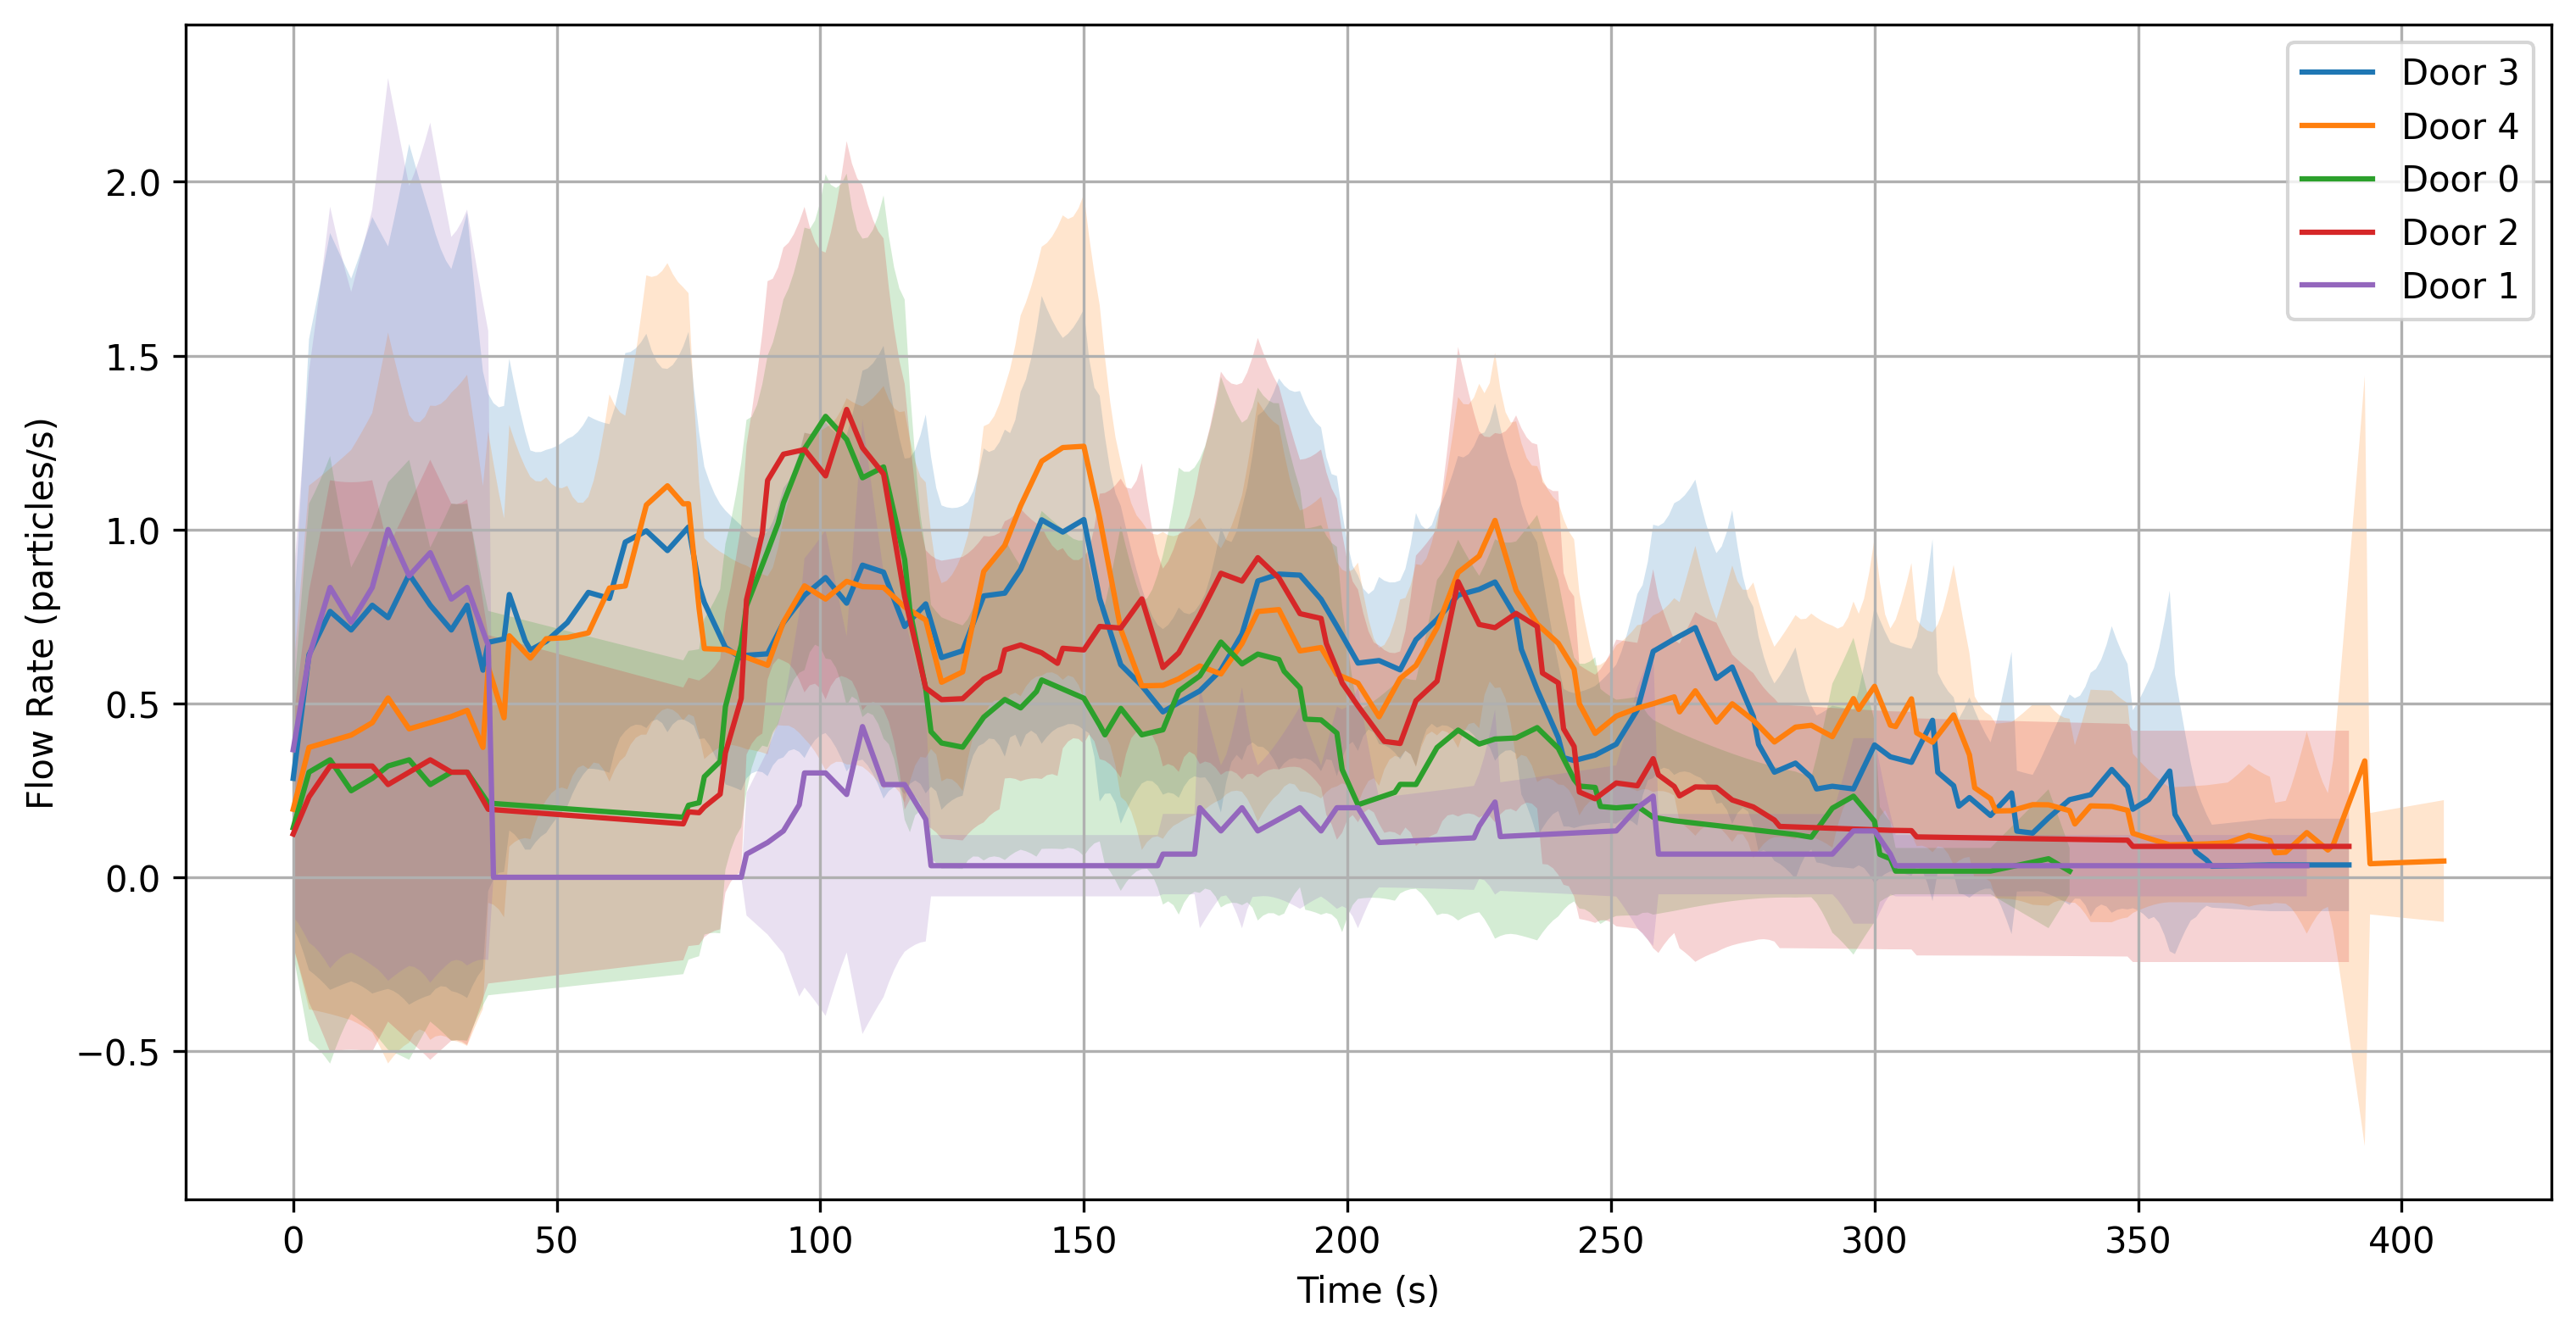
\includegraphics[width=0.9\textwidth]{img/door_flow_rates_t_20_&_p_0.00.png}
    \caption{Caudal promedio de partículas para $p=0.00$}
    \label{fig:caudal_p000}
\end{figure}

Esta comparación revela que la priorización de la distancia ($p = 1.00$) resulta en una evacuación más rápida pero potencialmente congestionada, mientras que la priorización de la densidad ($p = 0.00$) produce una evacuación más lenta pero con menor congestión en las salidas. El caso intermedio ($p = 0.50$) representa un compromiso entre velocidad de evacuación y distribución del flujo.

\subsubsection{Densidad en función de $p$}

\begin{figure}[H]
    \centering
    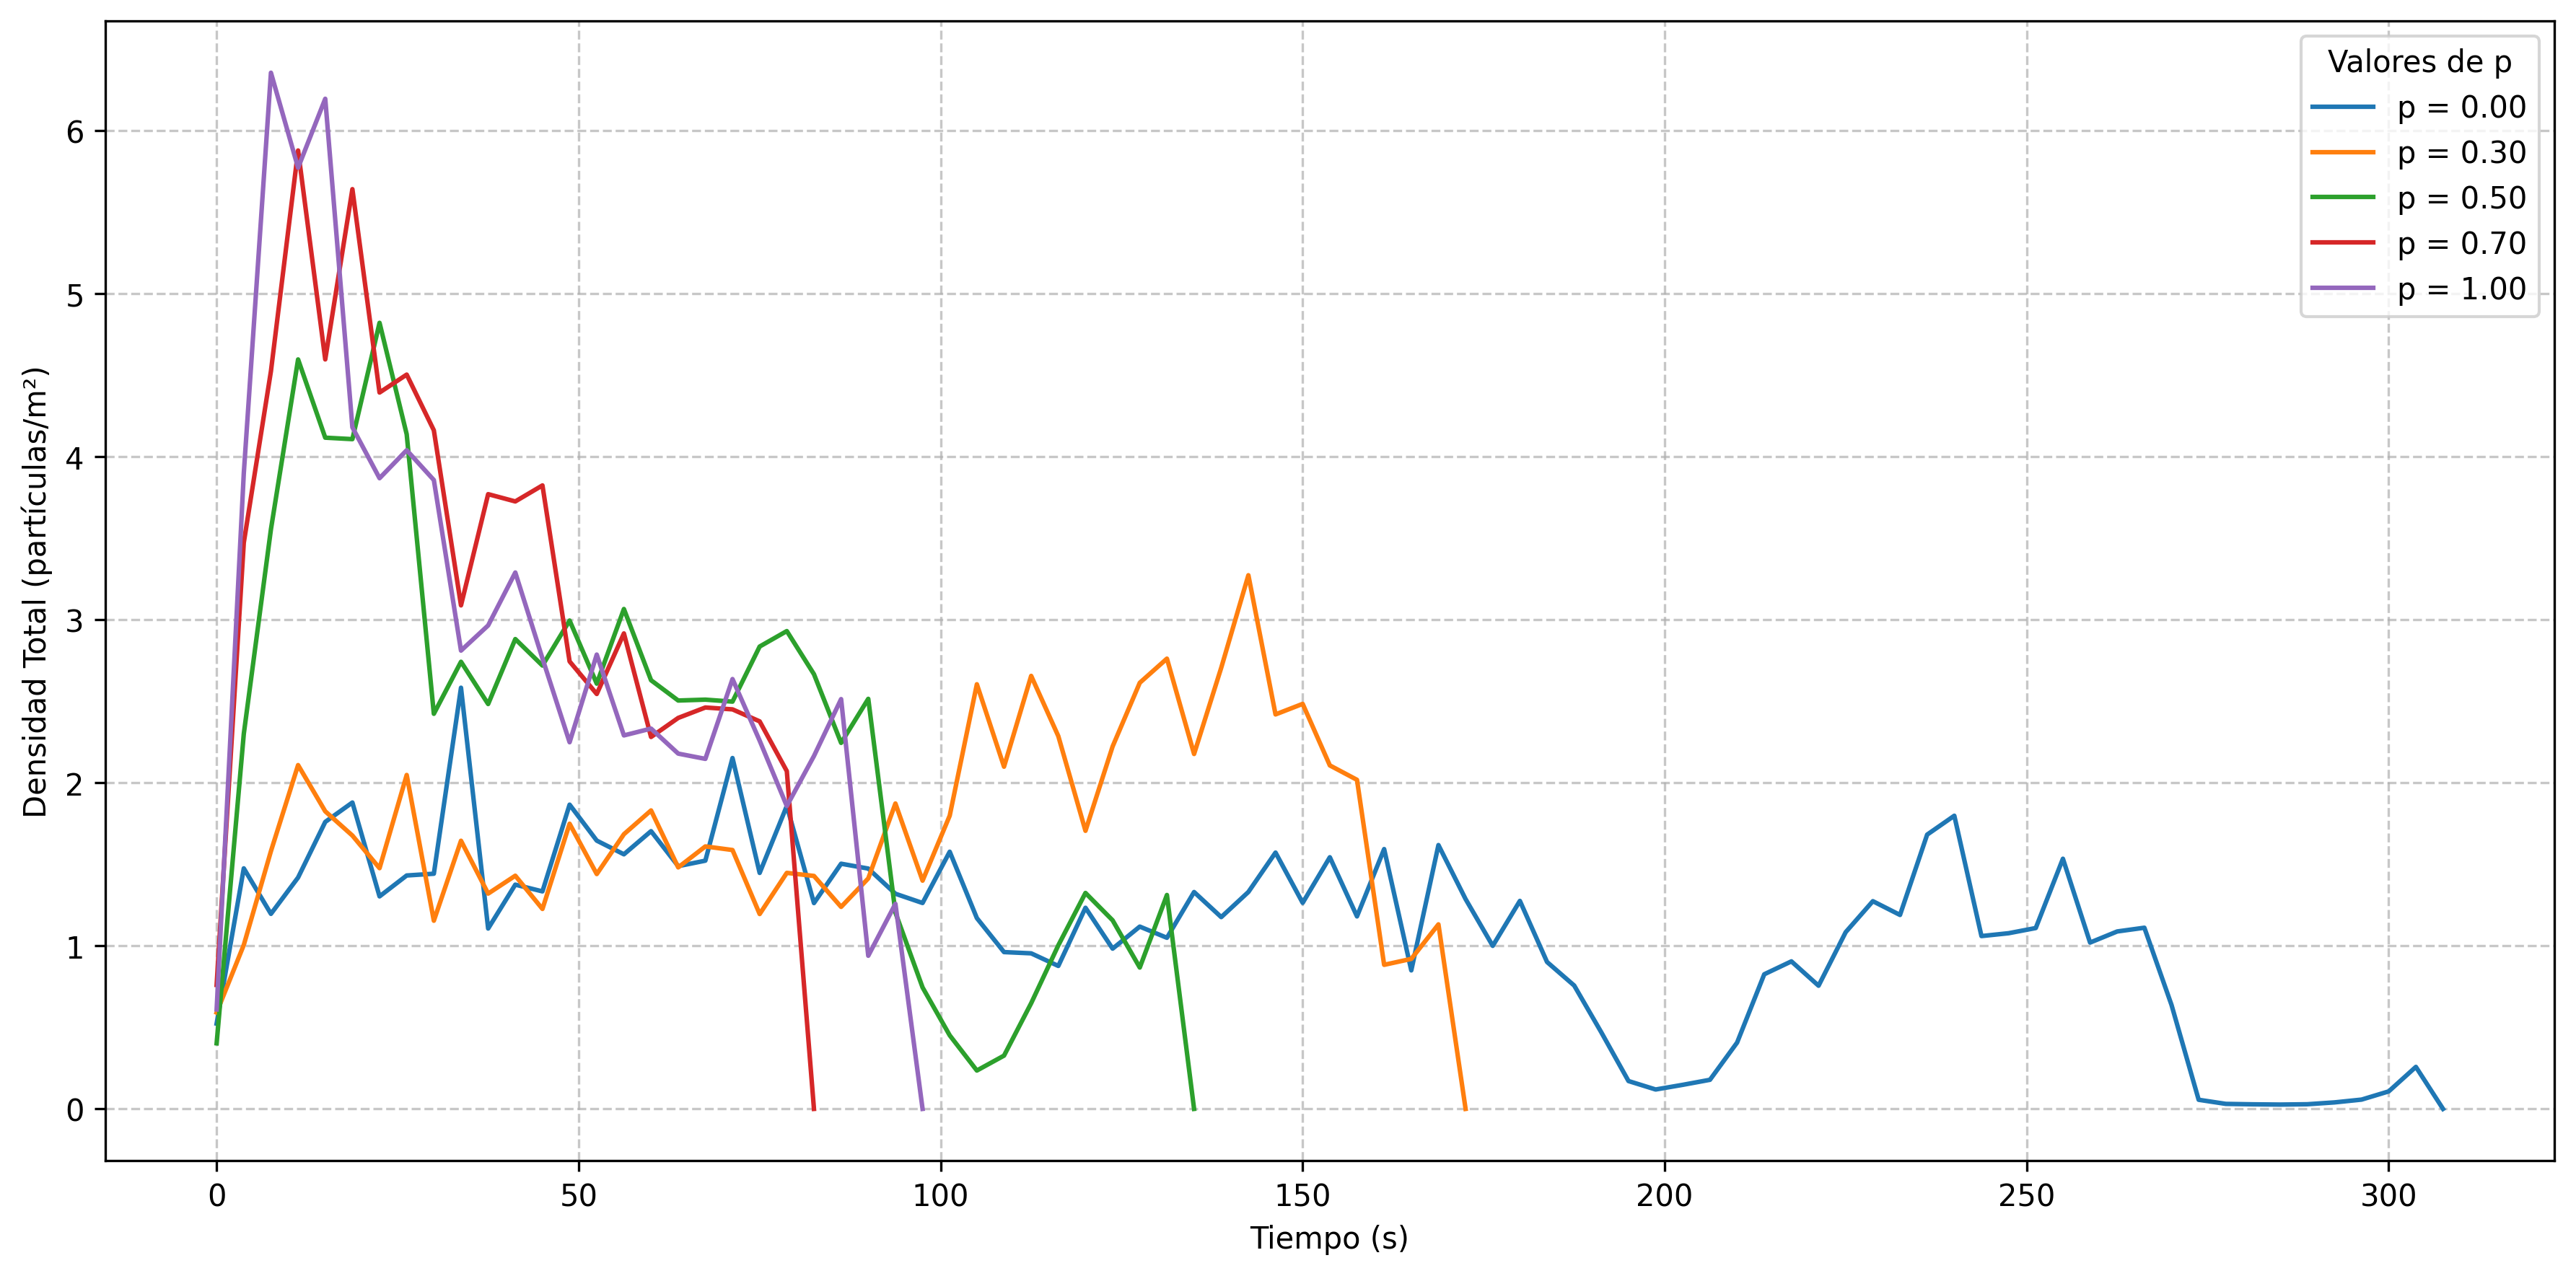
\includegraphics[width=0.9\textwidth]{img/density_vs_time_t45.png}
    \caption{Densidad en función del tiempo para $ct=45$}
    \label{fig:flow_p100}
\end{figure}

\begin{figure}[H]
    \centering
    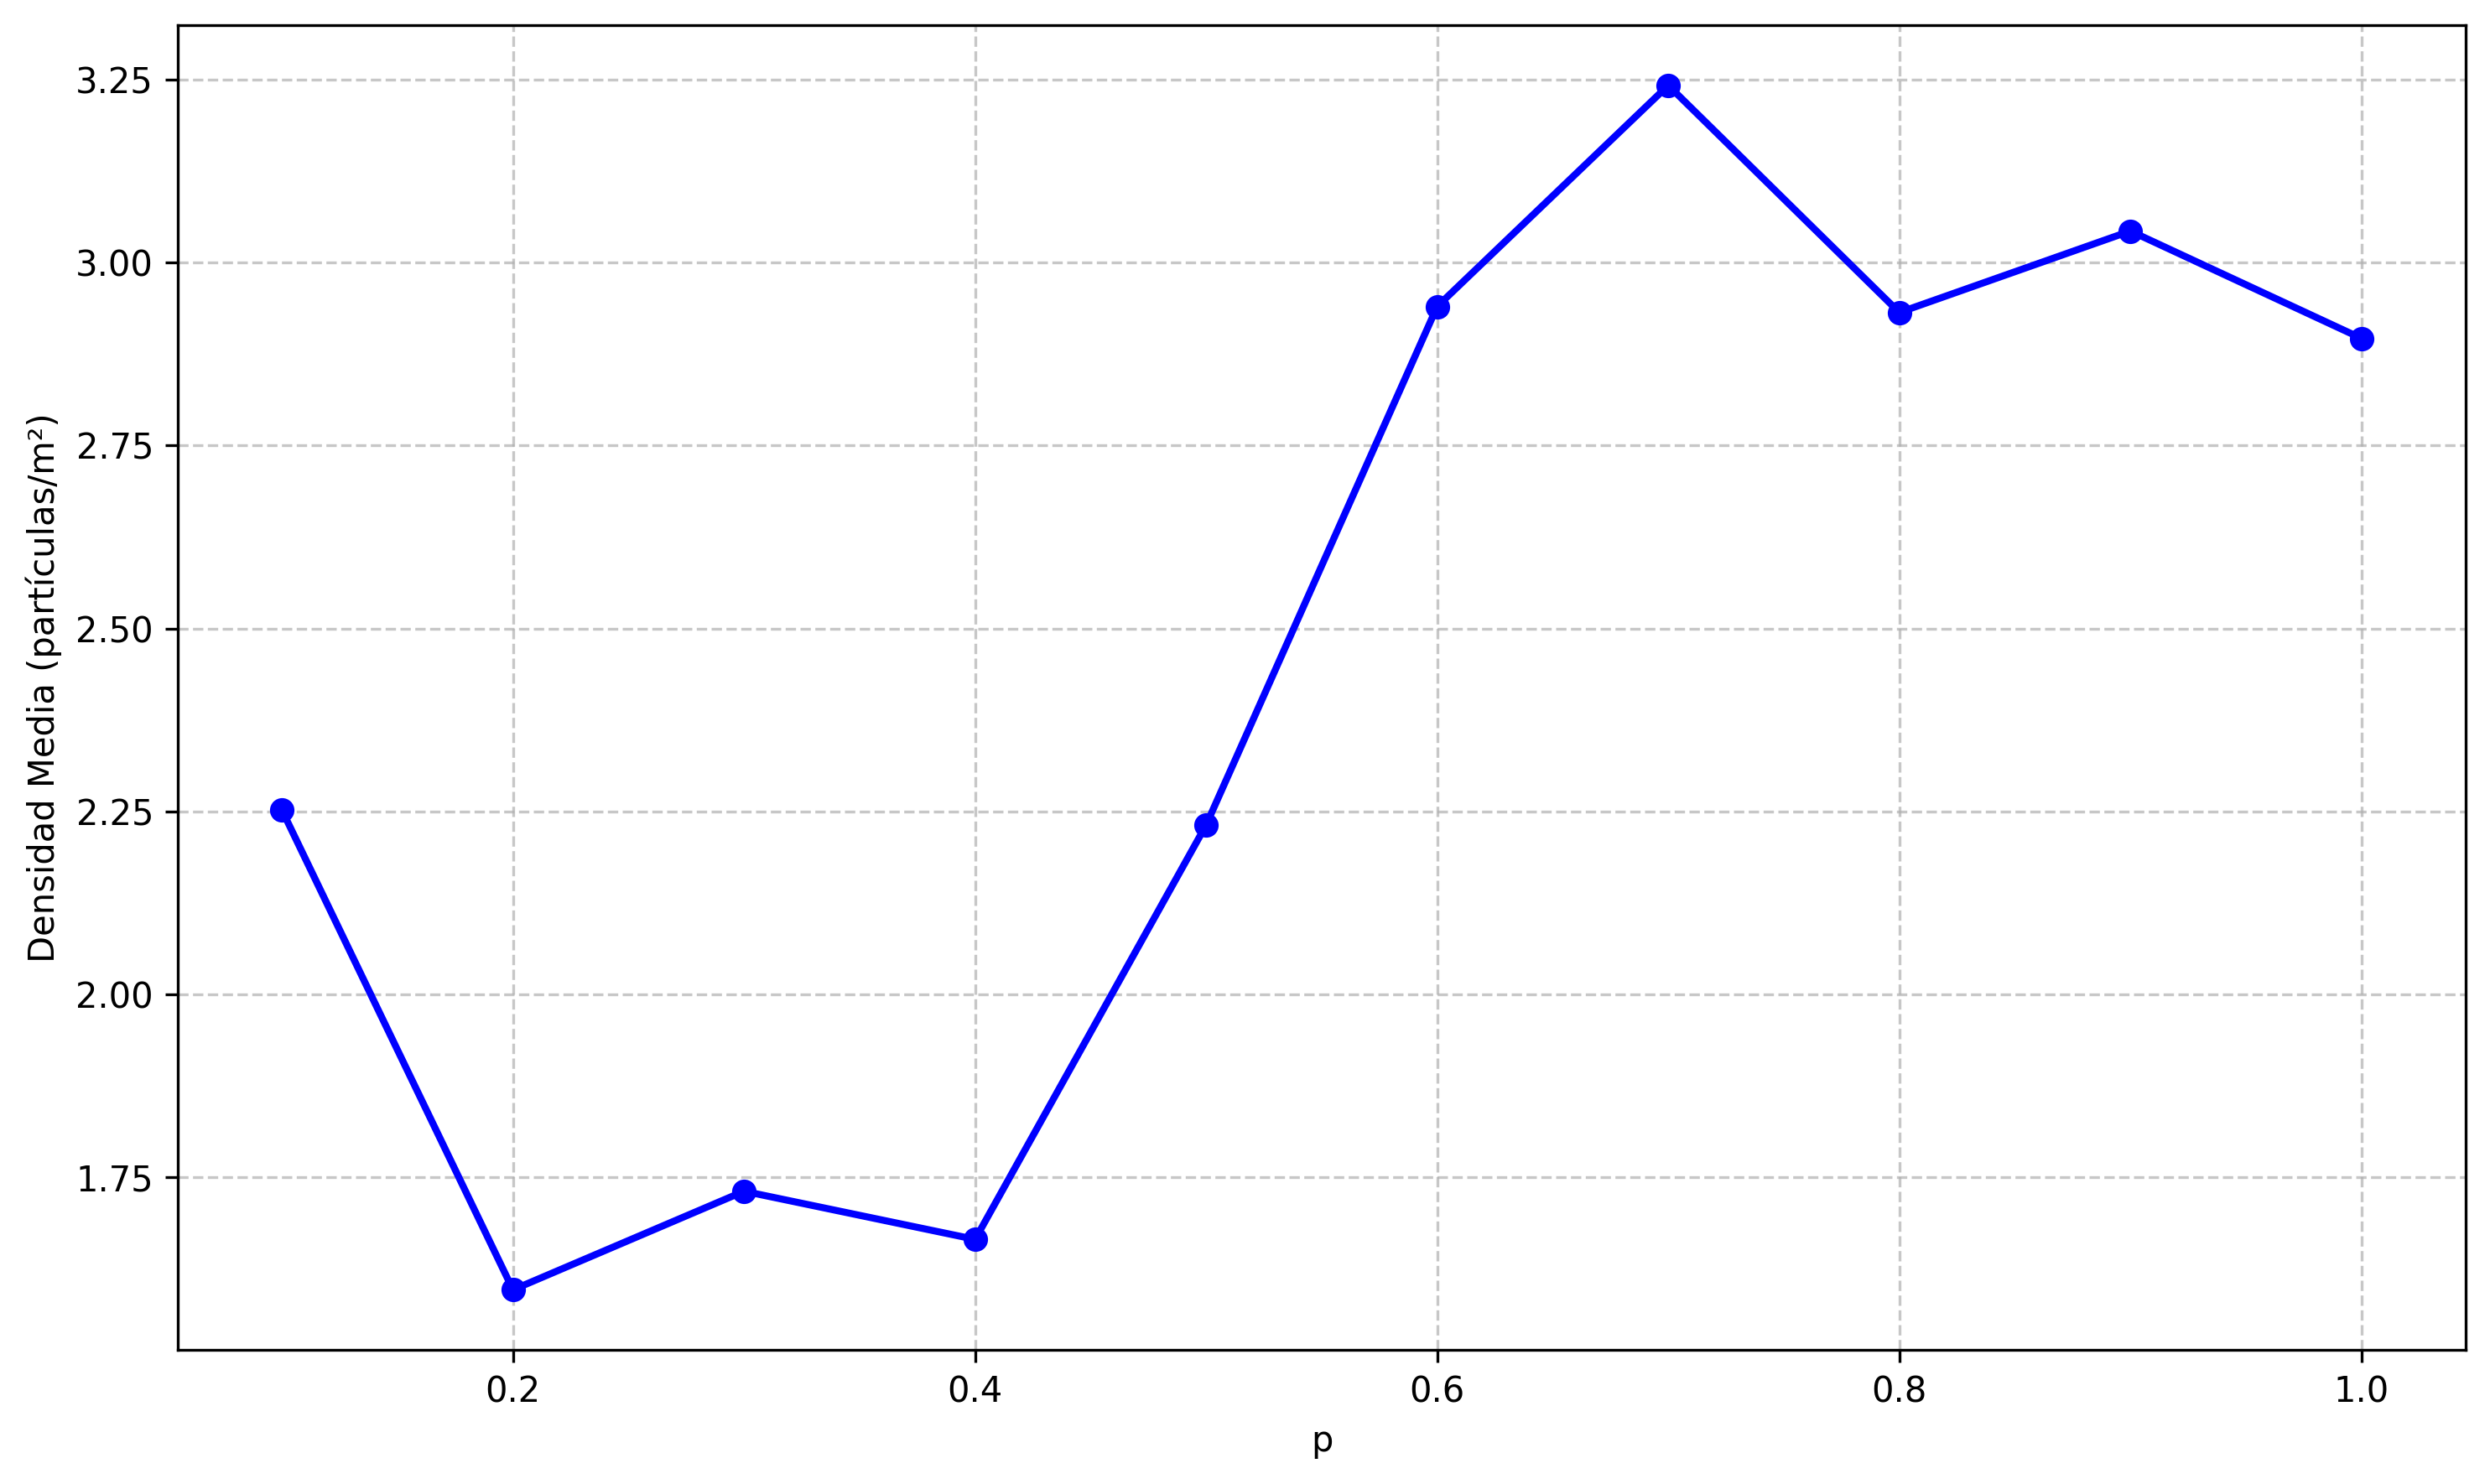
\includegraphics[width=0.9\textwidth]{img/average_density_t45.png}
    \caption{Densidad media en función de $p$ para $ct=45$}
    \label{fig:flow_p100}
\end{figure}

Se puede observar que a medida que la densidad es menor decisiva, la densidad en las puertas es mayor. Esto se debe a que las partículas ya desde el comienzo tienen una fuerte preferencia por la puerta más cercana y siempre la siguen eligiendo sin importar la densidad que haya en la misma, lo que conlleva a que en ciertas puertas se concentre mucha gente pro varios intervalos de tiempo, ya que todos van a la puerta más cercana sin tener en cuenta tanto la densidad de personas cerca de la misma. 
También podemos notar que al tornarse más relevante la densidad, todas las puertas tienen aproximadamente la misma densidad ya que los agentes se van reubicando de manera tal de ir a la puerta menos densa.

\subsection{Análisis de Densidades por Puerta}

Se analizaron tres escenarios diferentes variando el parámetro $p$ de la heurística de selección de puerta, manteniendo constante el tiempo de re-decisión ($ct=20s$) y el radio de medición ($r=3m$). Los resultados muestran patrones distintivos en la distribución de la densidad de partículas:

\subsubsection{Escenario 1: $p = 1.00$ (Prioridad Total a la Distancia)}

\begin{figure}[H]
    \centering
    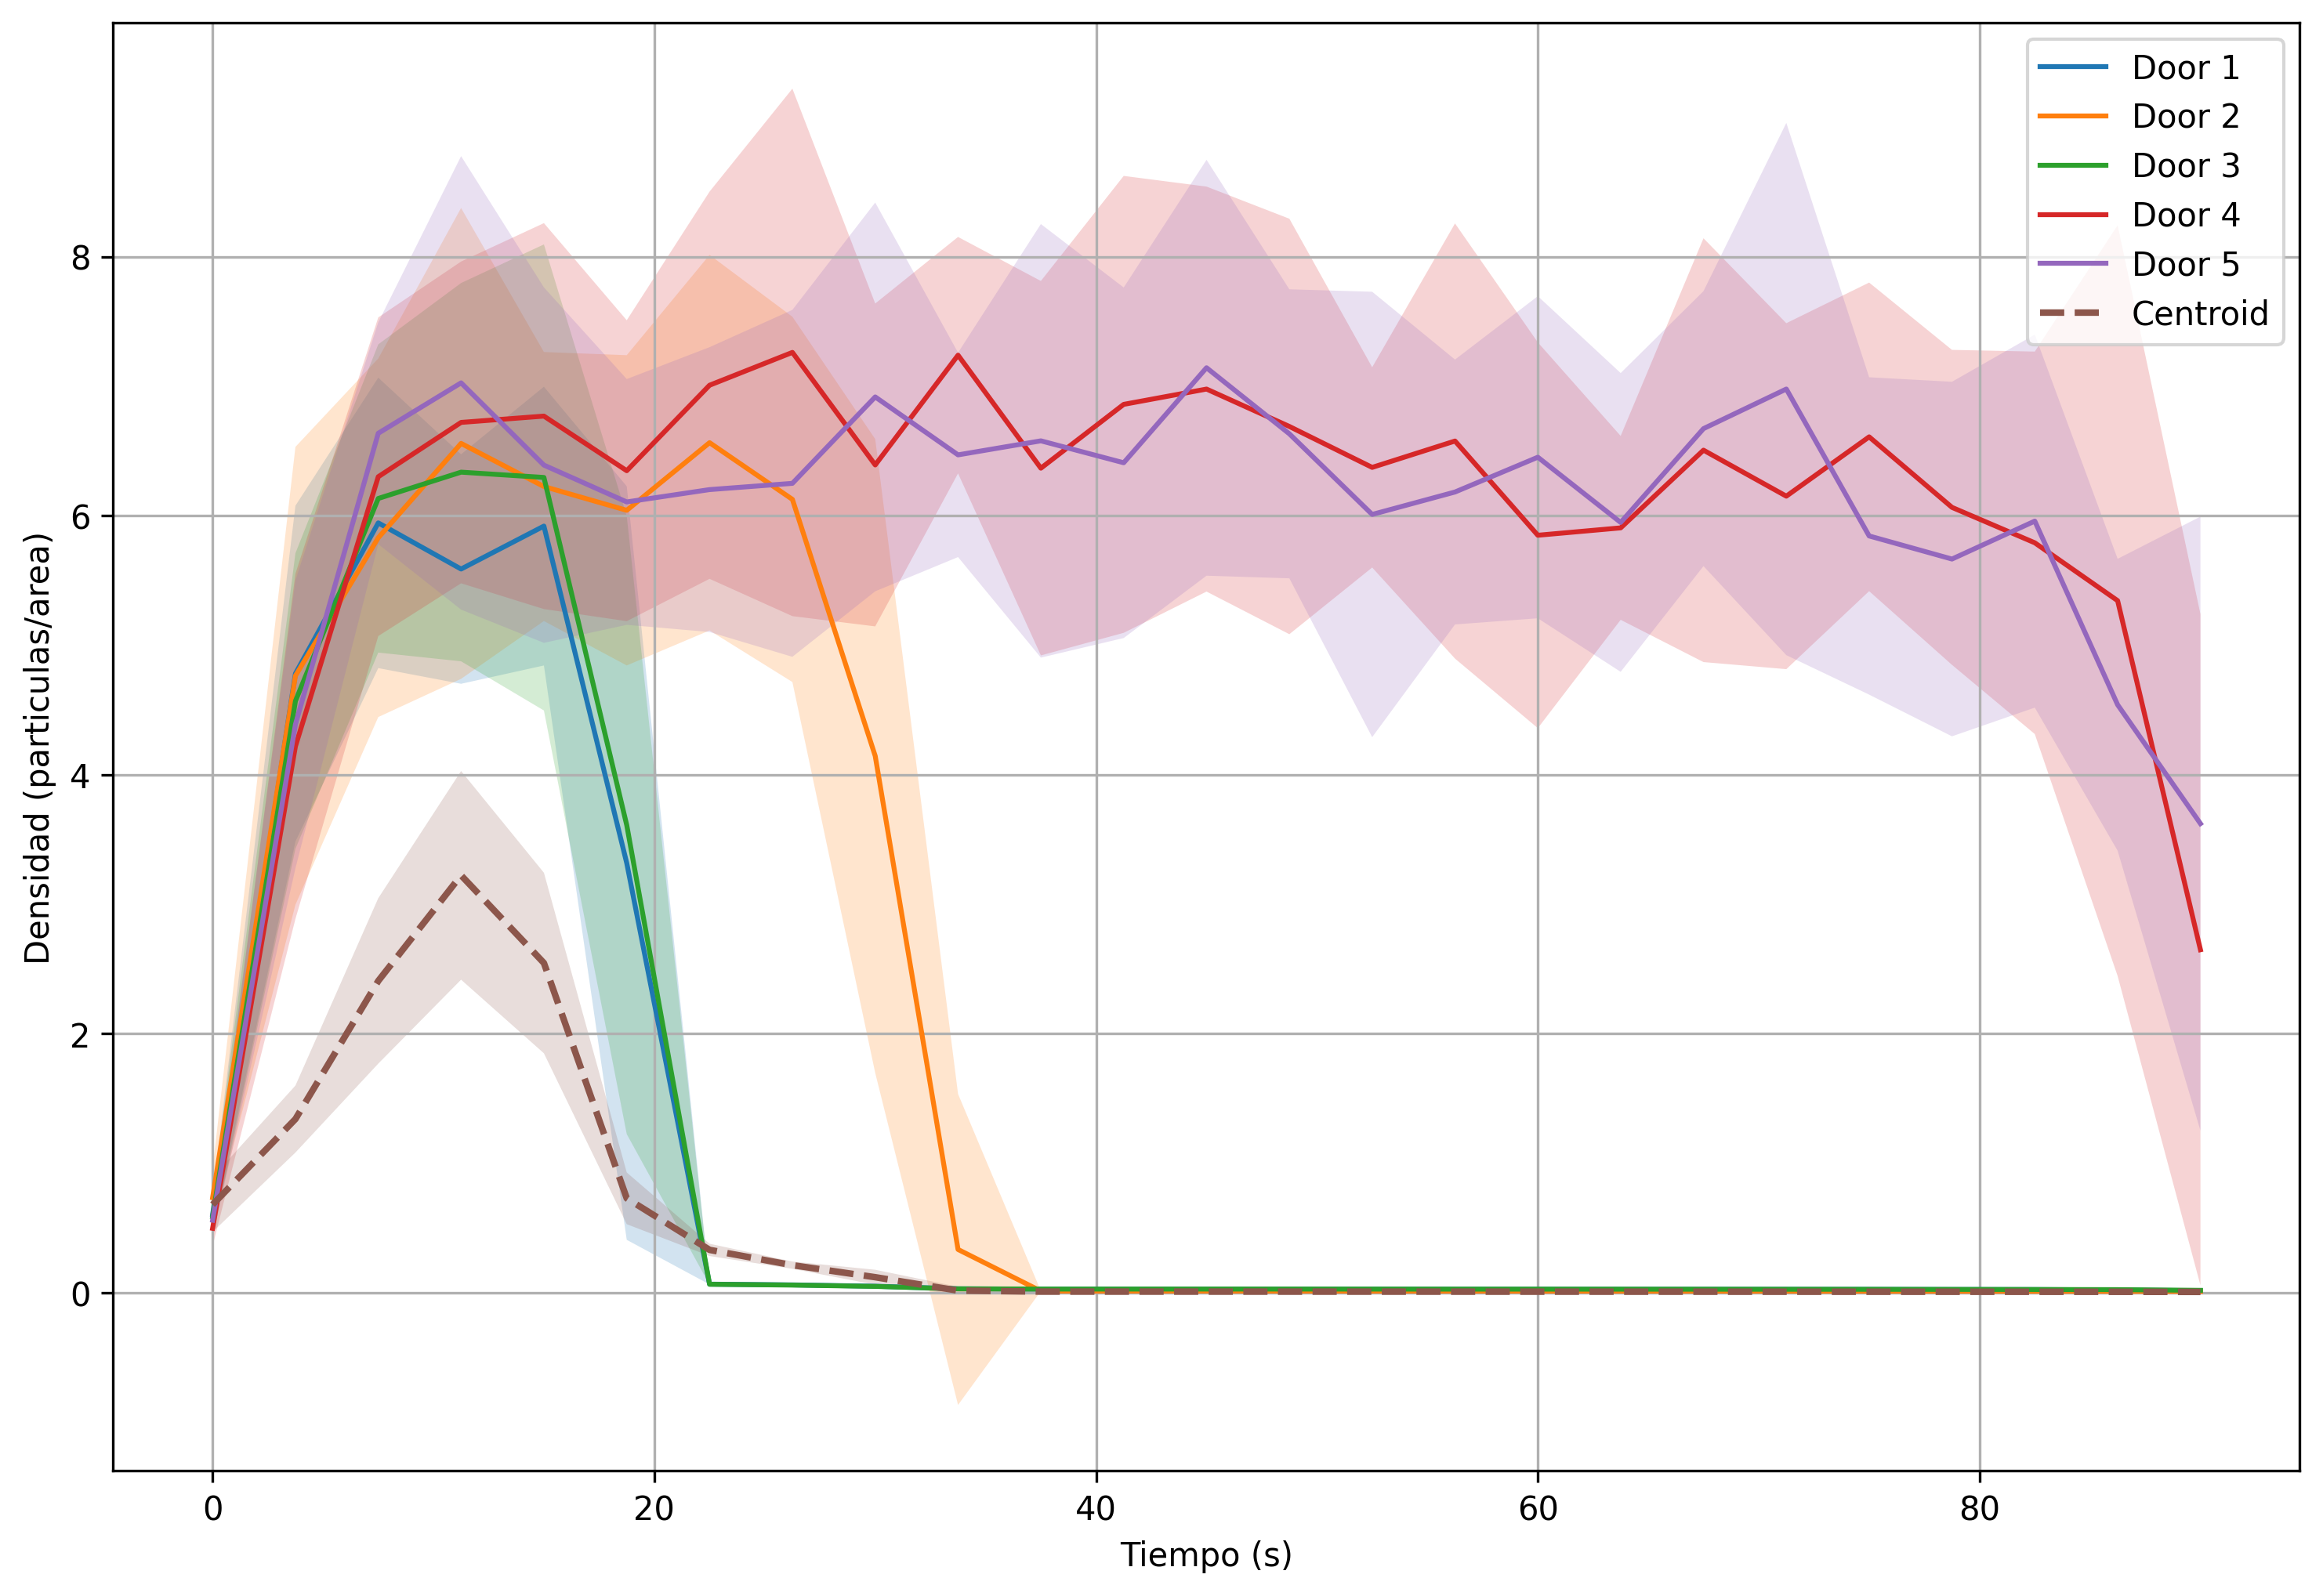
\includegraphics[width=0.9\textwidth]{img/circular_density_t_20_&_p_1.00.png}
    \caption{Densidad promedio de partículas en las proximidades de cada puerta para $p=1.00$. Las bandas sombreadas representan la desviación estándar sobre 15 realizaciones independientes.}
    \label{fig:densidad_p100}
\end{figure}

\begin{itemize}
    \item Las puertas 4 y 5 (laterales superiores) muestran las mayores densidades, alcanzando picos de aproximadamente 2.2 partículas/unidad de área alrededor de los 20 segundos.
    \item Las puertas 1, 2 y 3 presentan densidades significativamente menores, con máximos cercanos a 1 partícula/unidad de área.
    \item La evacuación se completa relativamente rápido (aproximadamente 90 segundos).
    \item Se observa una clara asimetría en la utilización de las salidas, con sobrecarga en las puertas más cercanas al centro del recinto.
\end{itemize}

\subsubsection{Escenario 2: $p = 0.50$ (Balance entre Distancia y Densidad)}

\begin{figure}[H]
    \centering
    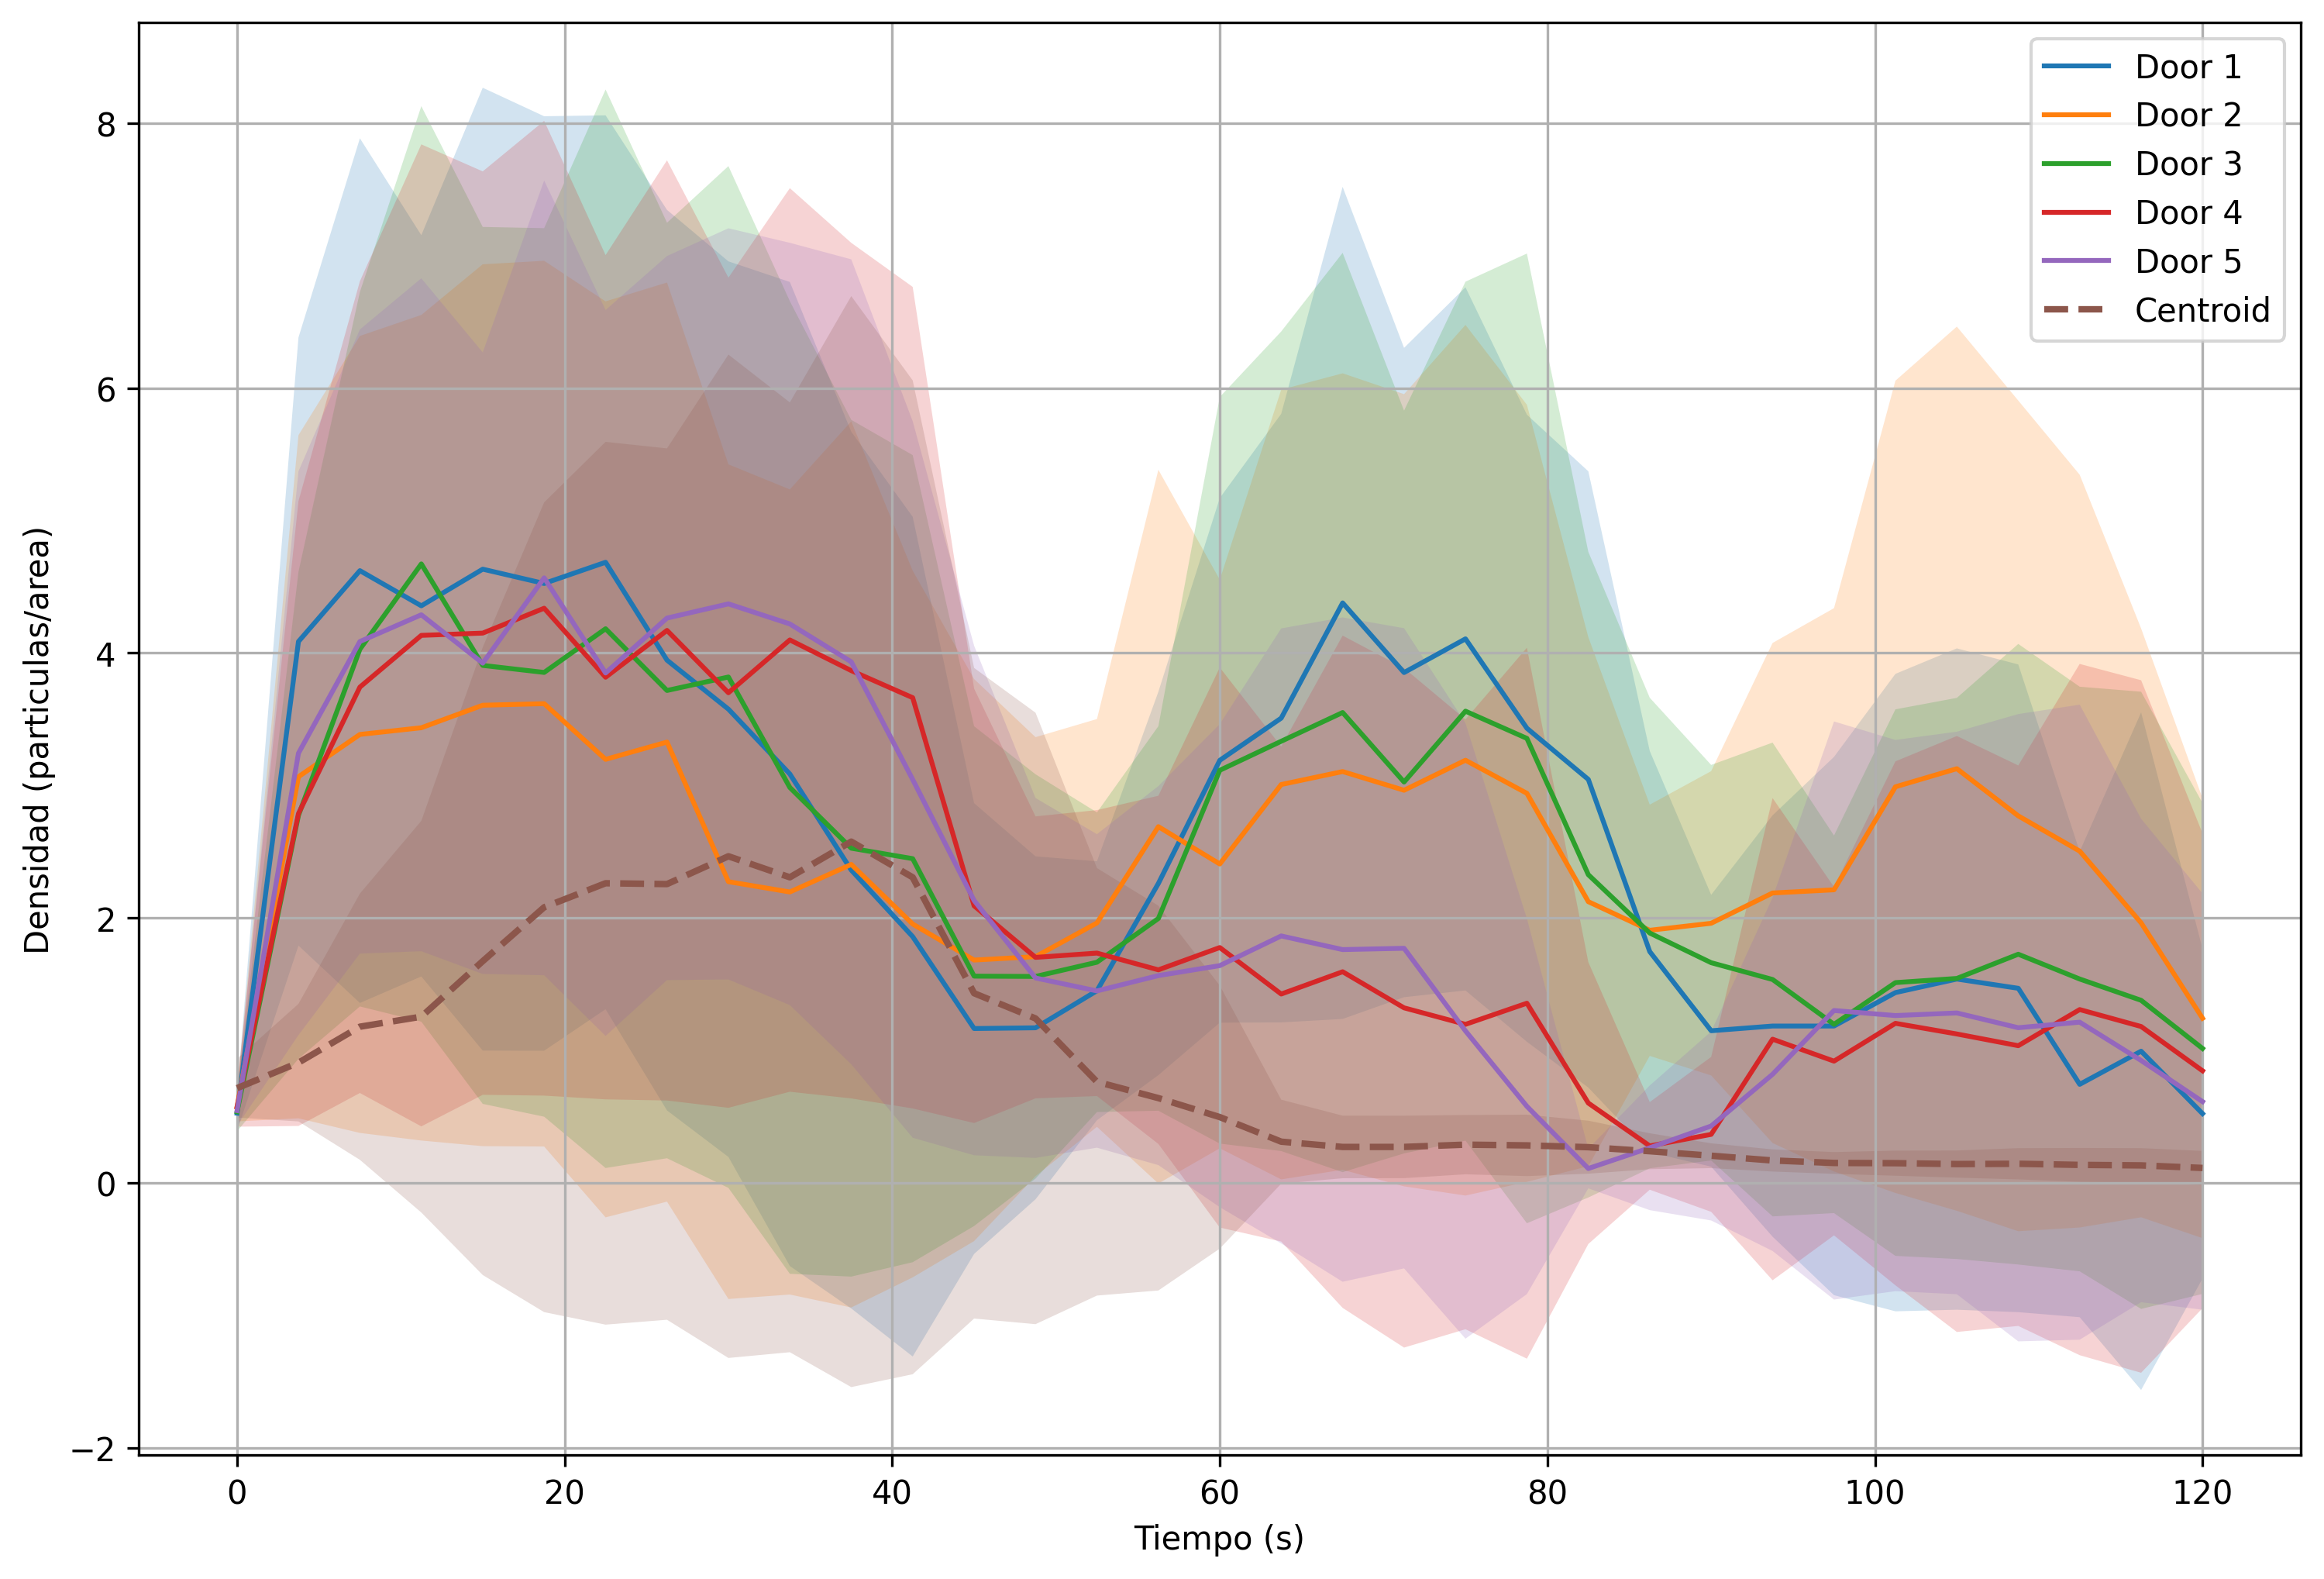
\includegraphics[width=0.9\textwidth]{img/circular_density_t_20_&_p_0.50.png}
    \caption{Densidad promedio de partículas en las proximidades de cada puerta para $p=0.50$. Las bandas sombreadas representan la desviación estándar sobre 15 realizaciones independientes.}
    \label{fig:densidad_p050}
\end{figure}

\begin{itemize}
    \item Las densidades máximas son menores que en el caso anterior, alcanzando aproximadamente 1.5 partículas/unidad de área.
    \item La distribución entre puertas es más uniforme, con fluctuaciones menos pronunciadas.
    \item El tiempo total de evacuación aumenta (aproximadamente 120 segundos).
    \item Se observan oscilaciones en las densidades, indicando que los agentes alternan entre diferentes salidas.
    \item El centroide de densidad muestra menor variabilidad, sugiriendo una distribución más equilibrada de la masa de agentes.
\end{itemize}

\subsubsection{Escenario 3: $p = 0.00$ (Prioridad Total a la Densidad)}

\begin{figure}[H]
    \centering
    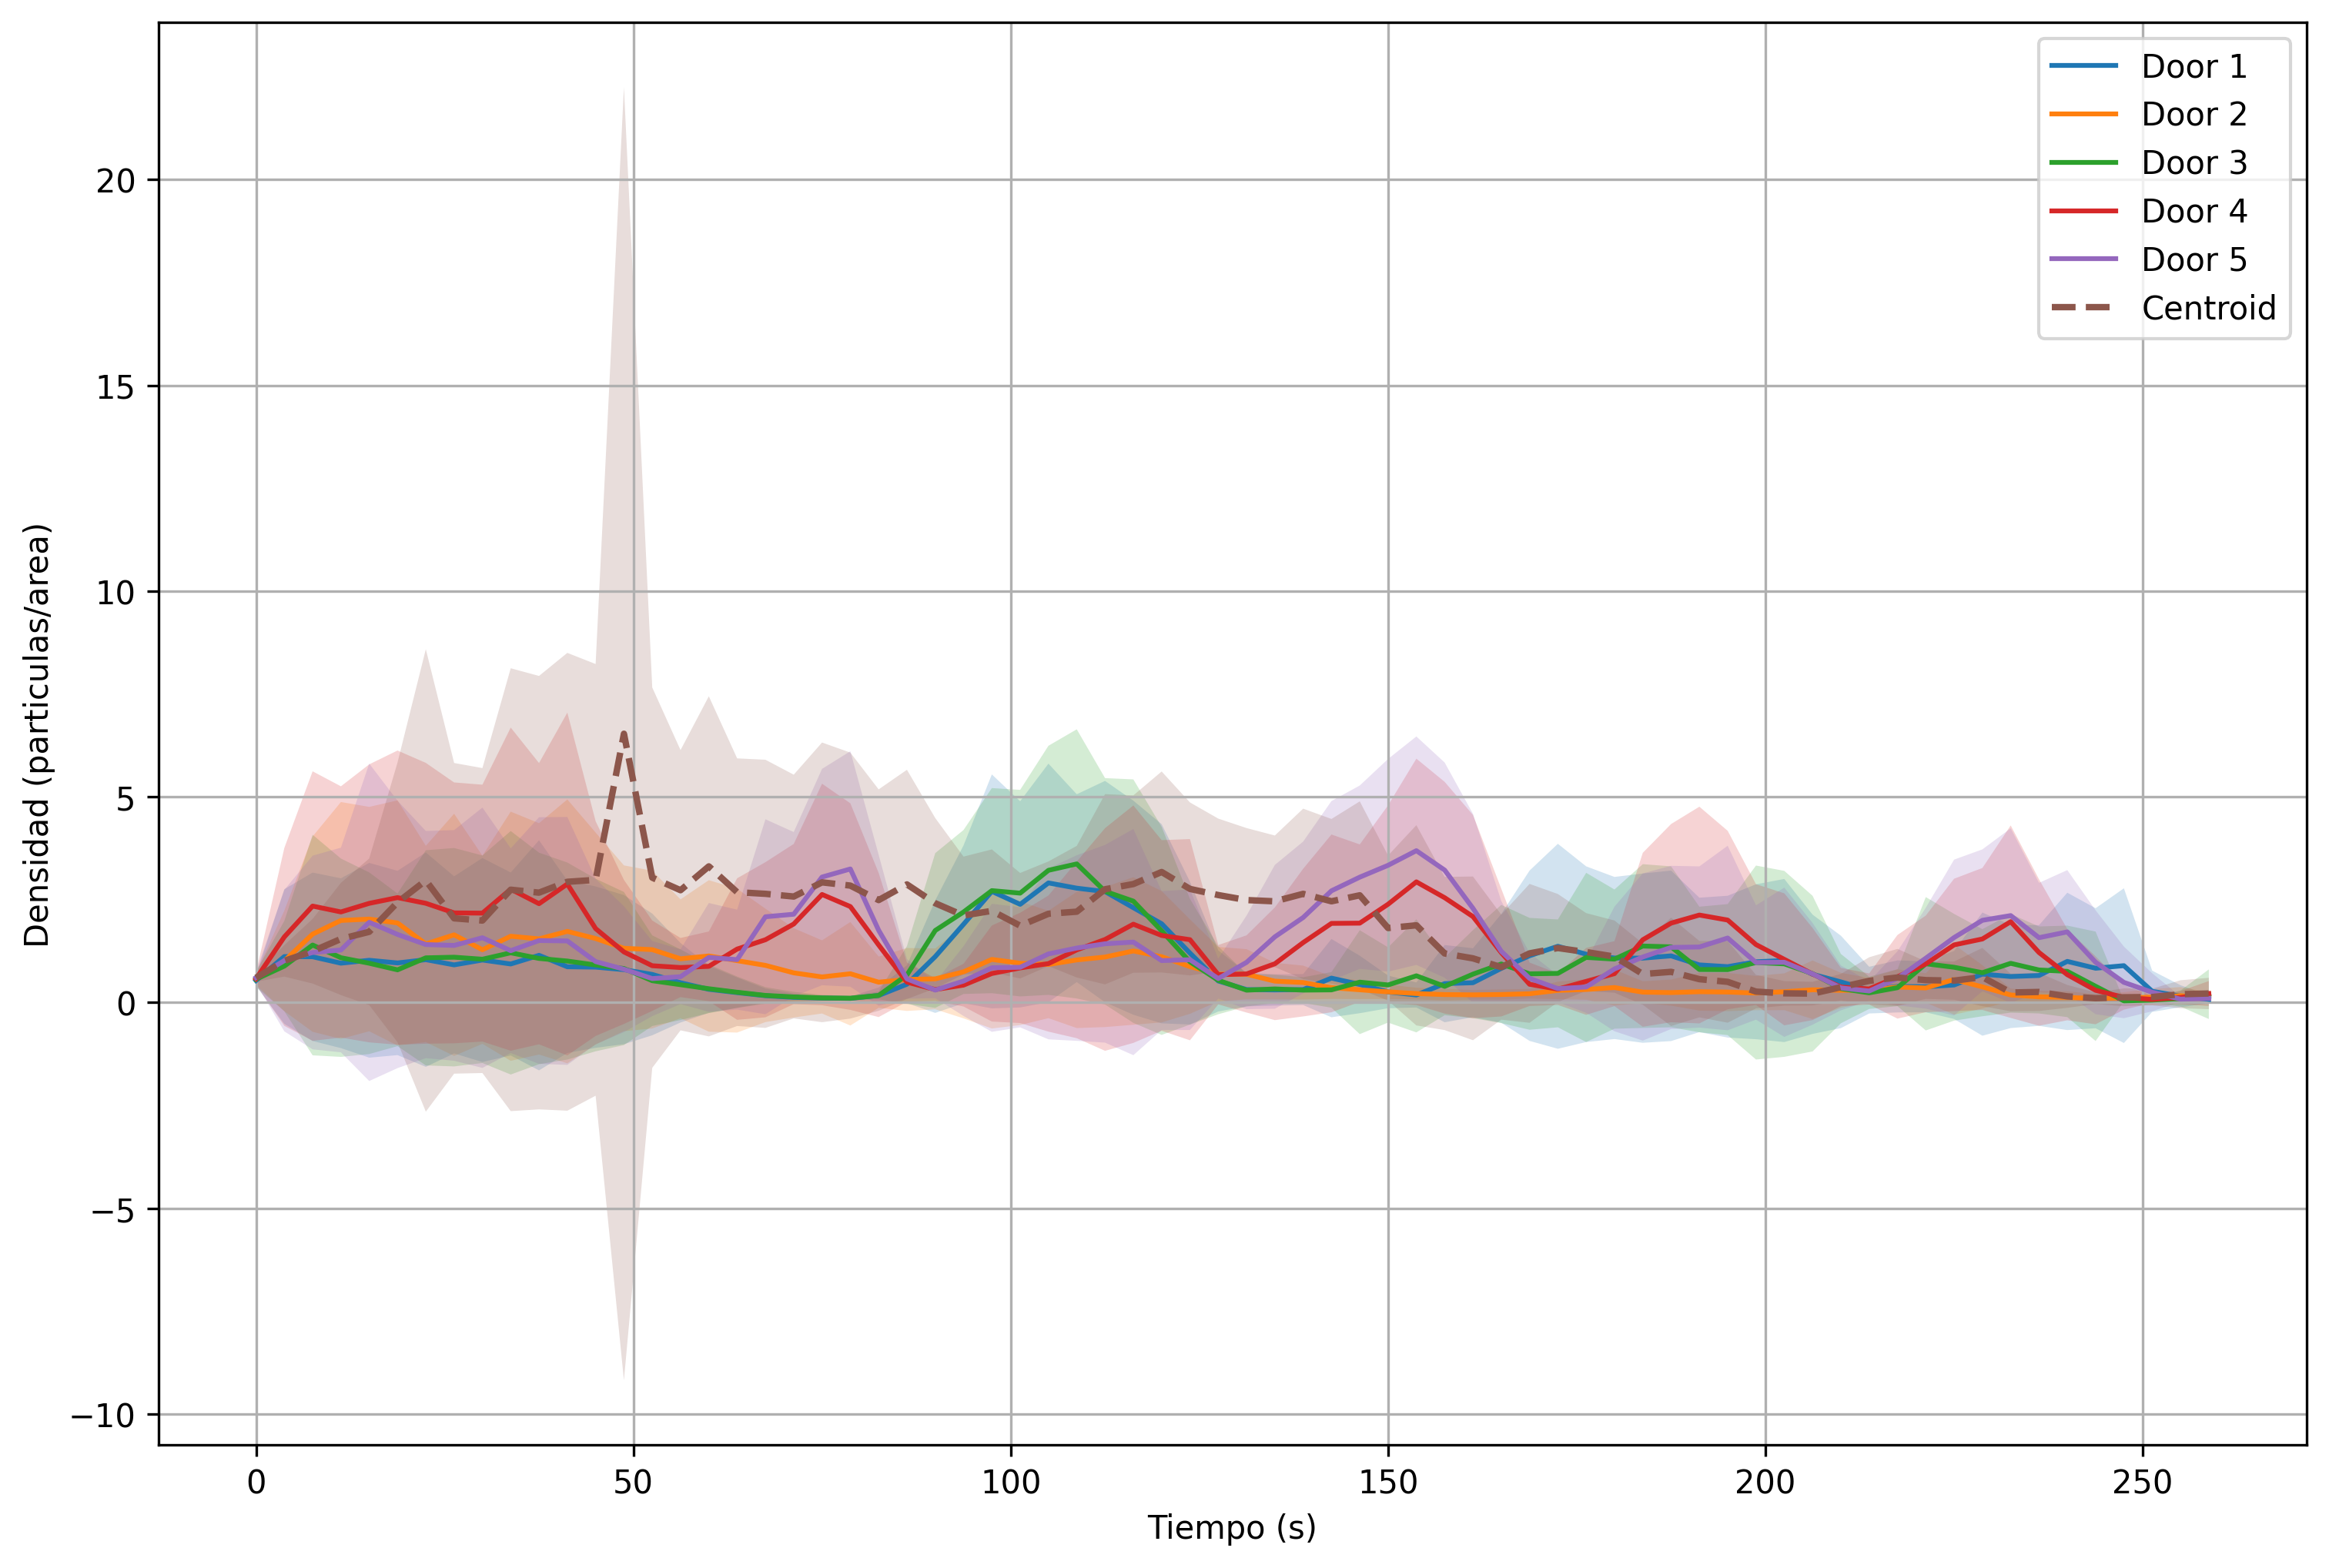
\includegraphics[width=0.9\textwidth]{img/circular_density_t_20_&_p_0.00.png}
    \caption{Densidad promedio de partículas en las proximidades de cada puerta para $p=0.00$}
    \label{fig:densidad_p000}
\end{figure}

\begin{itemize}
    \item Las densidades máximas son las más bajas de los tres casos (aproximadamente 1.2 partículas/unidad de área).
    \item Se observa una mayor variabilidad temporal en las densidades de cada puerta.
    \item El tiempo de evacuación es significativamente mayor (más de 250 segundos).
    \item Las curvas muestran múltiples oscilaciones, indicando frecuentes cambios en la elección de salida por parte de los agentes.
    \item El comportamiento es más errático, con períodos de densidad casi nula seguidos de picos moderados.
\end{itemize}

\subsubsection{Coeficiente de uniformidad en función de $p$}

\begin{figure}[H]
    \centering
    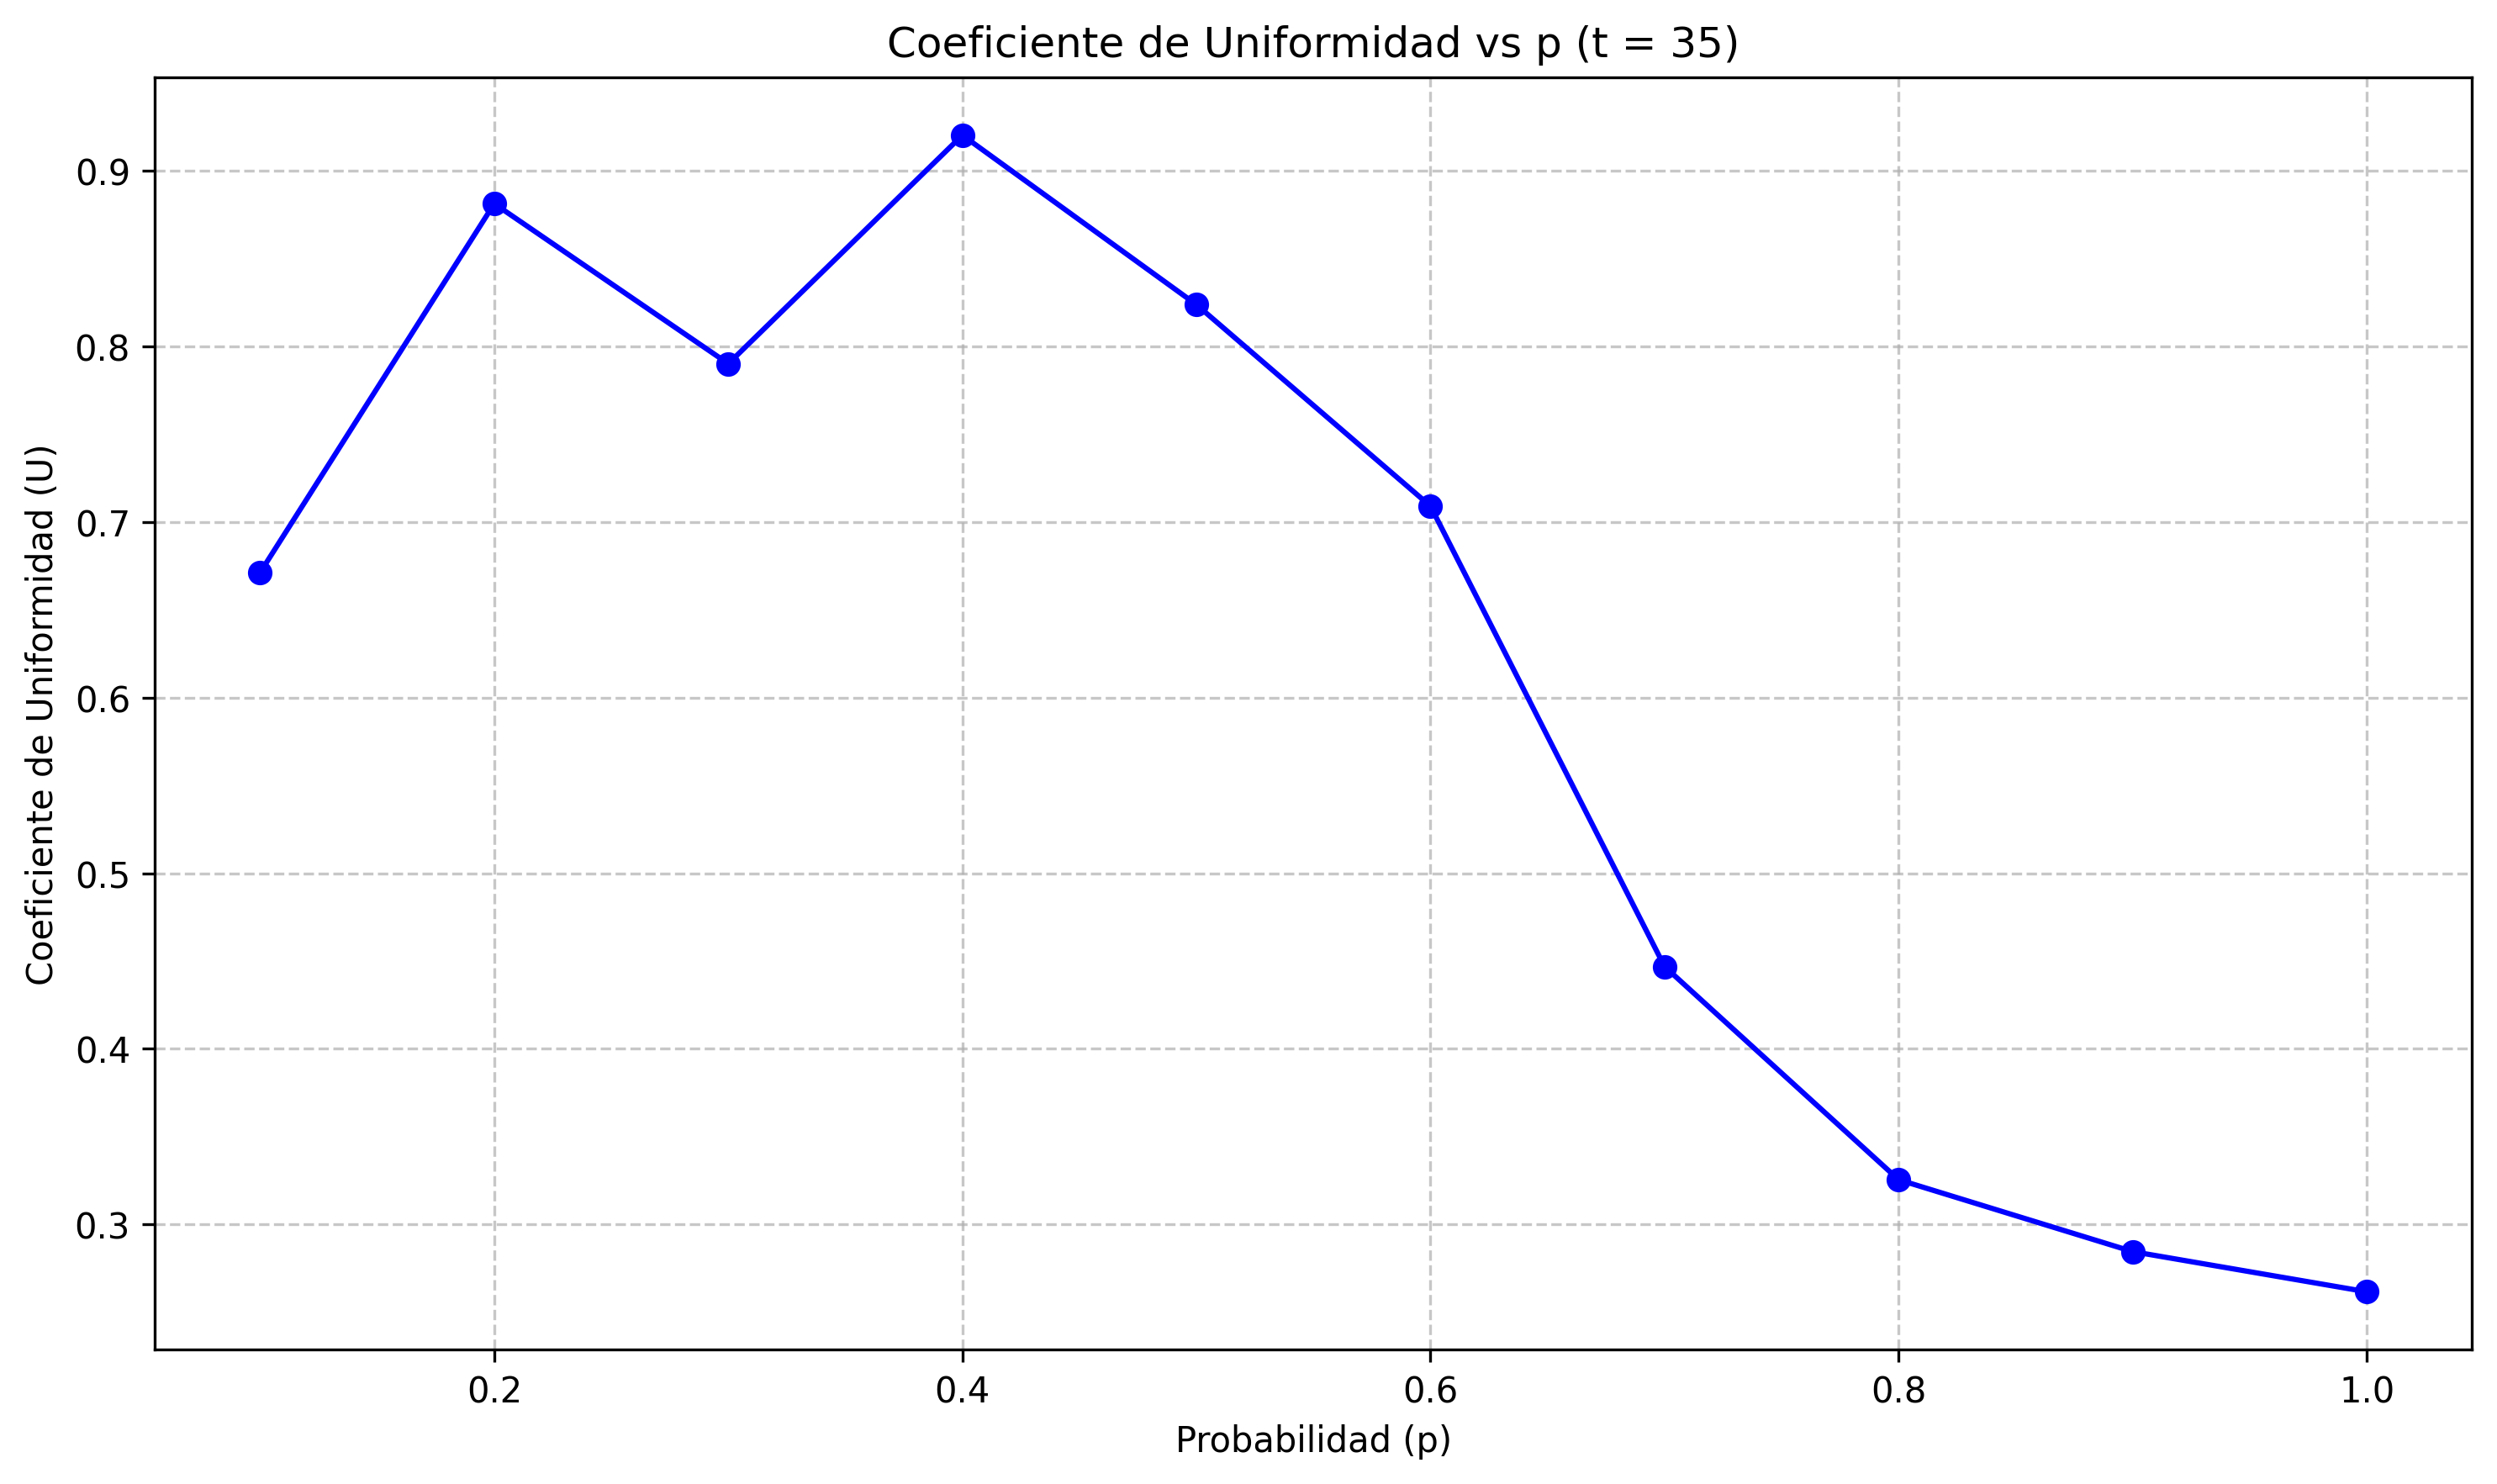
\includegraphics[width=0.9\textwidth]{img/uniformity_vs_p_t35.png}
    \caption{Coeficiente de uniformidad para $ct=35$}
    \label{fig:flow_p100}
\end{figure}
Podemos observar que a medida que aumenta el parámetro de ponderación $p$, haciendo que la distancia se vuelva más importante en la elección, el coeficiente de uniformidad decae. Esto se debe a que si la distancia es cada vez más relevante, los agentes se dirigirán a la puerta más cercana sin importar la densidad en la misma, haciendo que las puertas mas lejanas queden sin densidad, por lo que las puertas no se utilizan de manera pareja. Por el contrario, cuando la densidad se torna más relevante que la distancia, las partículas se distribuyen de manera más uniforme entre las puertas, ya que la densidad va cambiando y eso hace que ellas cambien la puerta elegida también. Es por eso que el coeficiente aumenta para estos casos.

\subsection{Análisis del Tiempo de Evacuación en función del Tiempo de Re-decisión}
\begin{figure}[H]
\centering
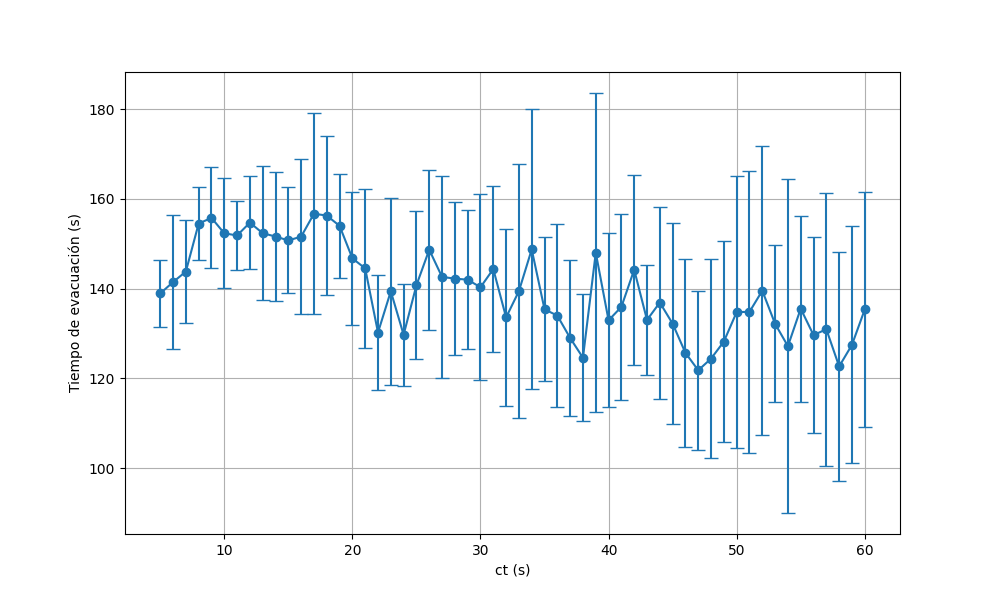
\includegraphics[width=0.9\textwidth]{img/evacuation_times_p_0.5.png}
\caption{Tiempo promedio de evacuación en función del tiempo de re-decisión ($ct$) para $p=0.50$}
\label{fig:evac_time_ct}
\end{figure}
El análisis del tiempo de evacuación en función del tiempo de re-decisión ($ct$) revela patrones interesantes en la dinámica del sistema. Para un valor fijo de $p=0.50$, que representa un balance entre la consideración de la distancia y la densidad en la elección de salidas, se observa una tendencia general decreciente en el tiempo de evacuación conforme aumenta el tiempo de re-decisión, aunque con considerable variabilidad.
En la región de tiempos de re-decisión cortos ($ct < 20s$), el tiempo de evacuación promedio se mantiene relativamente alto, oscilando alrededor de los 150 segundos. Esto sugiere que la frecuente reconsideración de la elección de salida puede resultar contraproducente, posiblemente debido a que los agentes cambian de objetivo antes de poder ejecutar efectivamente su plan de evacuación inicial.
En la región de tiempos de re-decisión más largos ($ct > 40s$), se aprecia una leve disminución en el tiempo promedio de evacuación, alcanzando valores cercanos a los 130 segundos, aunque con una variabilidad aún considerable. Esta mejora en el rendimiento podría explicarse por la mayor persistencia en la elección de salida, que permite a los agentes mantener sus trayectorias planificadas durante períodos más prolongados, y así, lograr salir del recinto.

\subsubsection{Caudal en función de $ct$}

\begin{figure}[H]
    \centering
    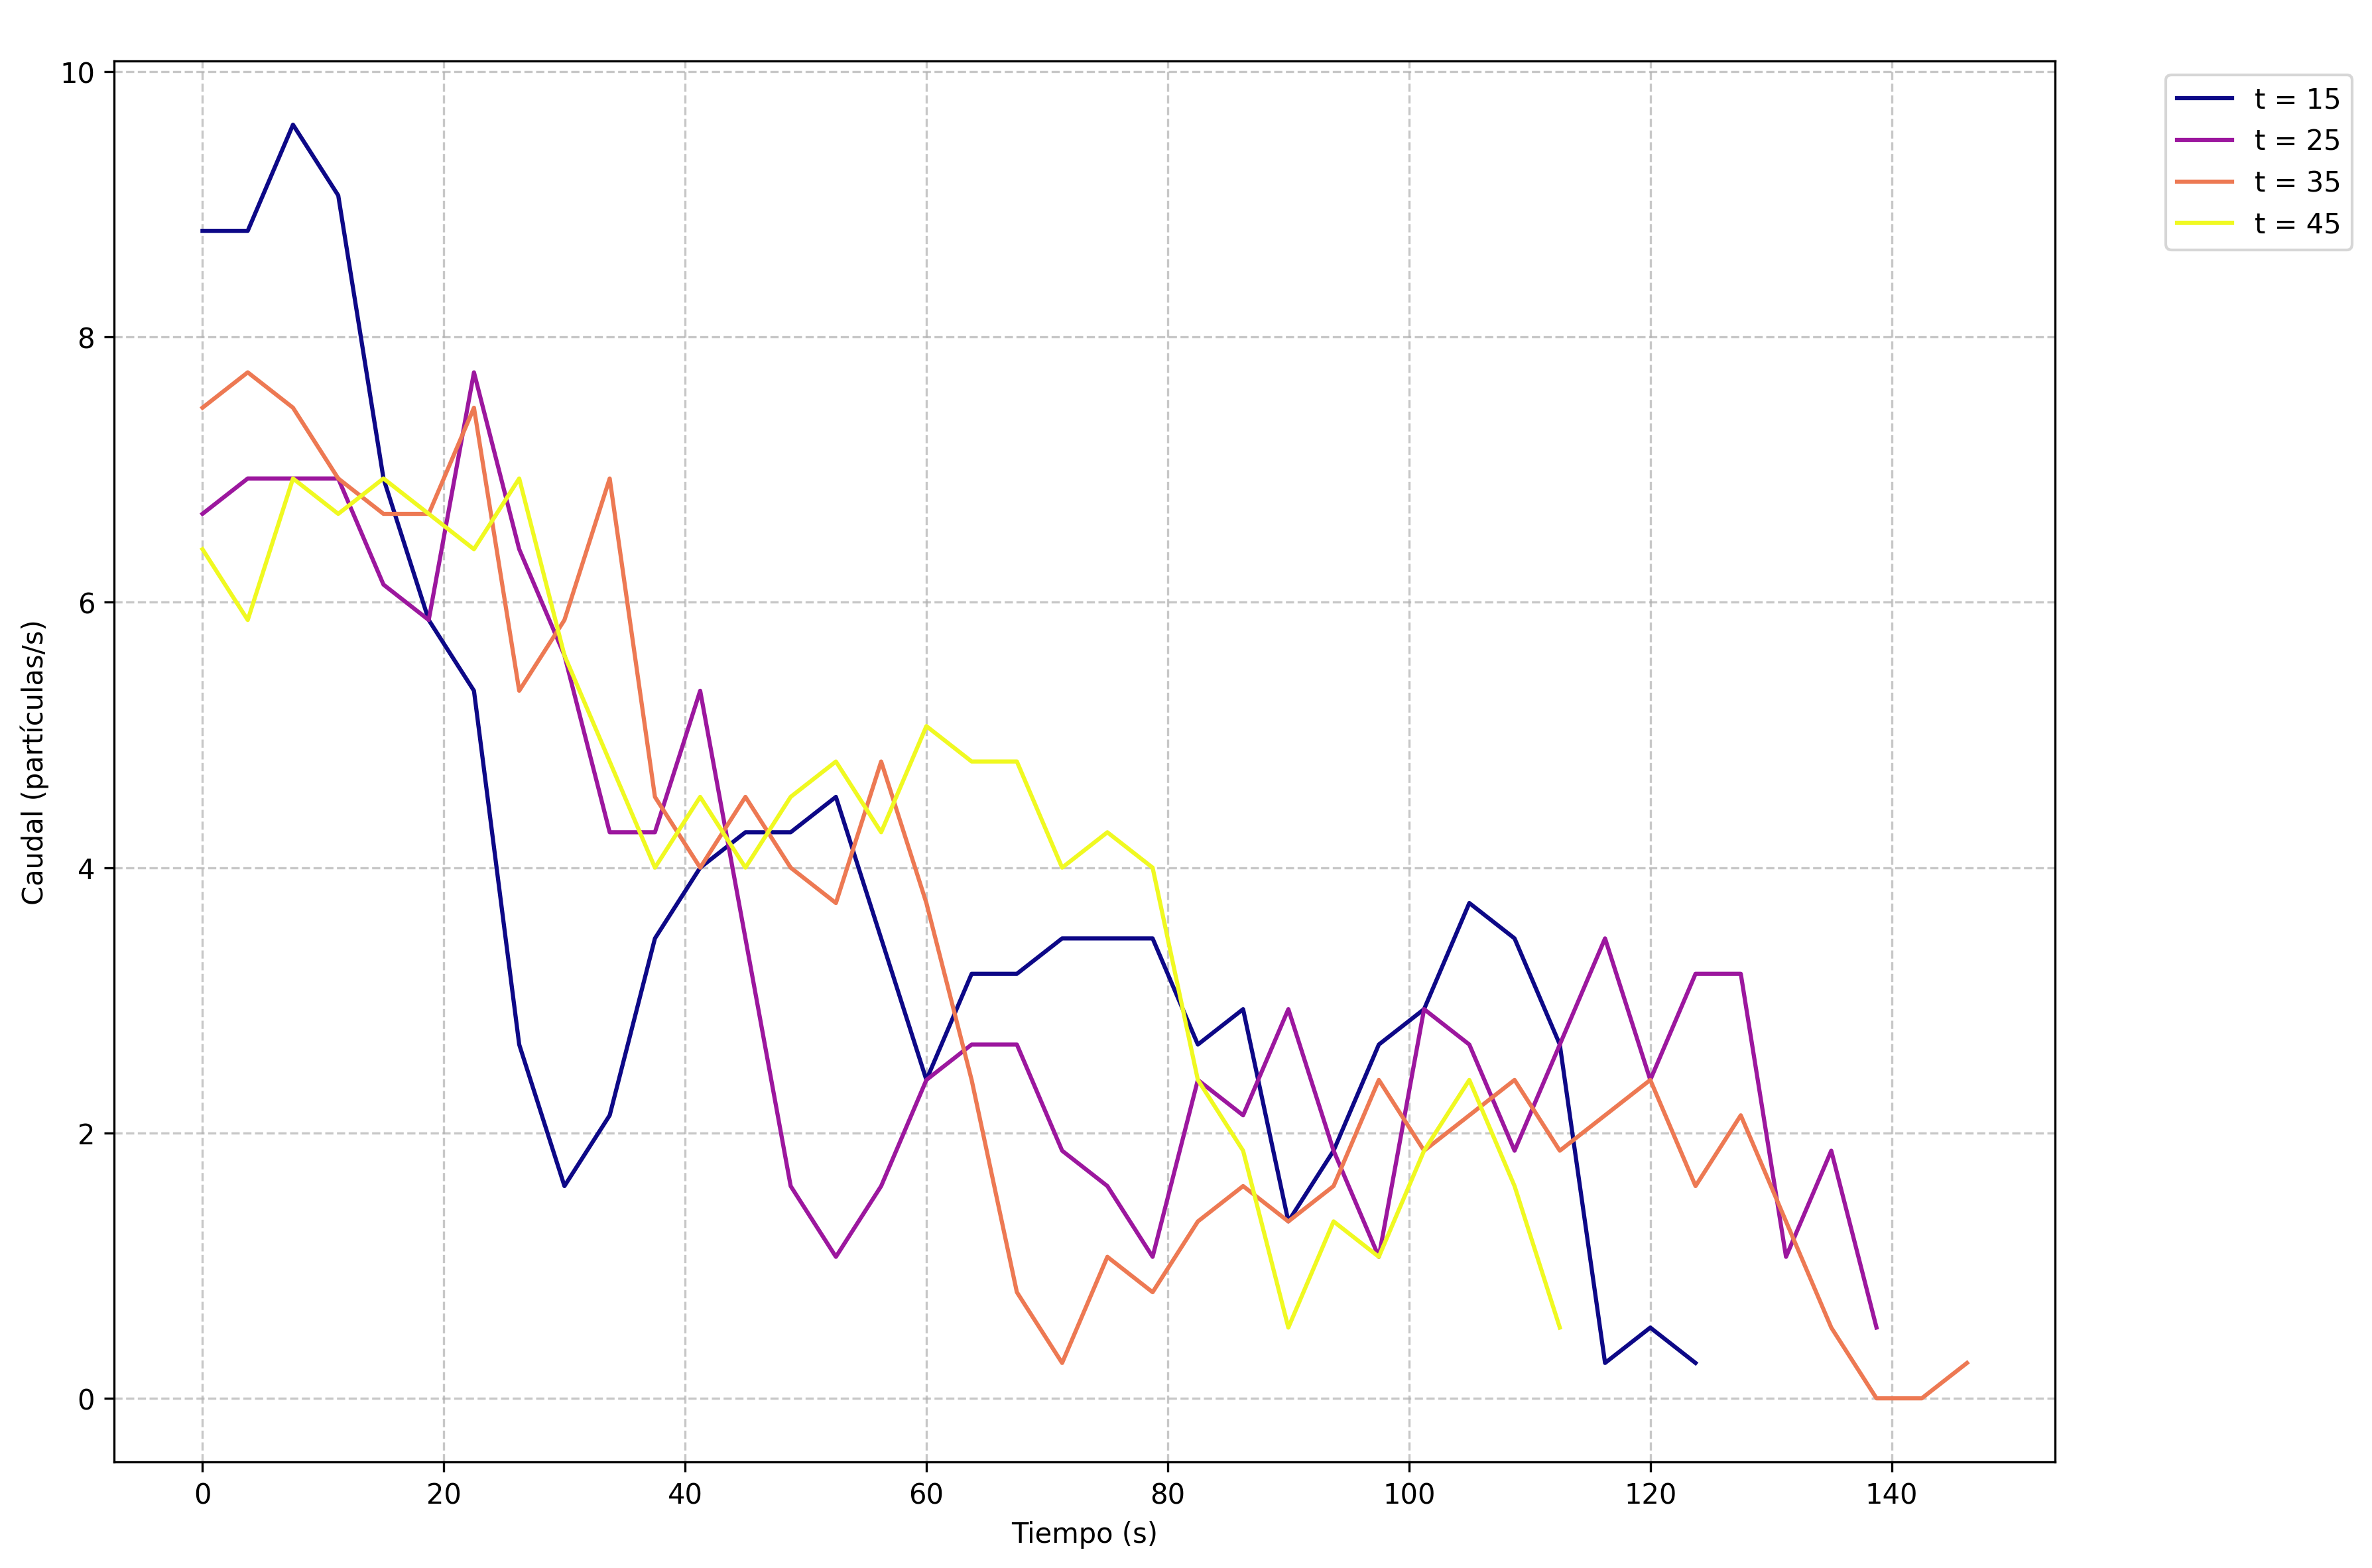
\includegraphics[width=0.9\textwidth]{img/flow_rates_p0.5.png}
    \caption{Caudal global en función del tiempo para $p=0.5$}
    \label{fig:flow_p100}
\end{figure}
Podemos notar que al aumentar el intervalo de tiempo para el cual vuelven a evaluar la elección de la puerta, el caudal tiene períodos donde resulta más estable y no está variando constantemente. Esto es porque al tener un tiempo de re-decisión alto, los agentes se ponen como objetivo la misma puerta por más tiempo. Teniendo en cuenta que usamos $p=0.5$ la densidad influye en la misma medida que la distancia, es por eso que se observan algunas fluctuaciones en el caudal.

\subsubsection{Densidad en función de $ct$}

\begin{figure}[H]
    \centering
    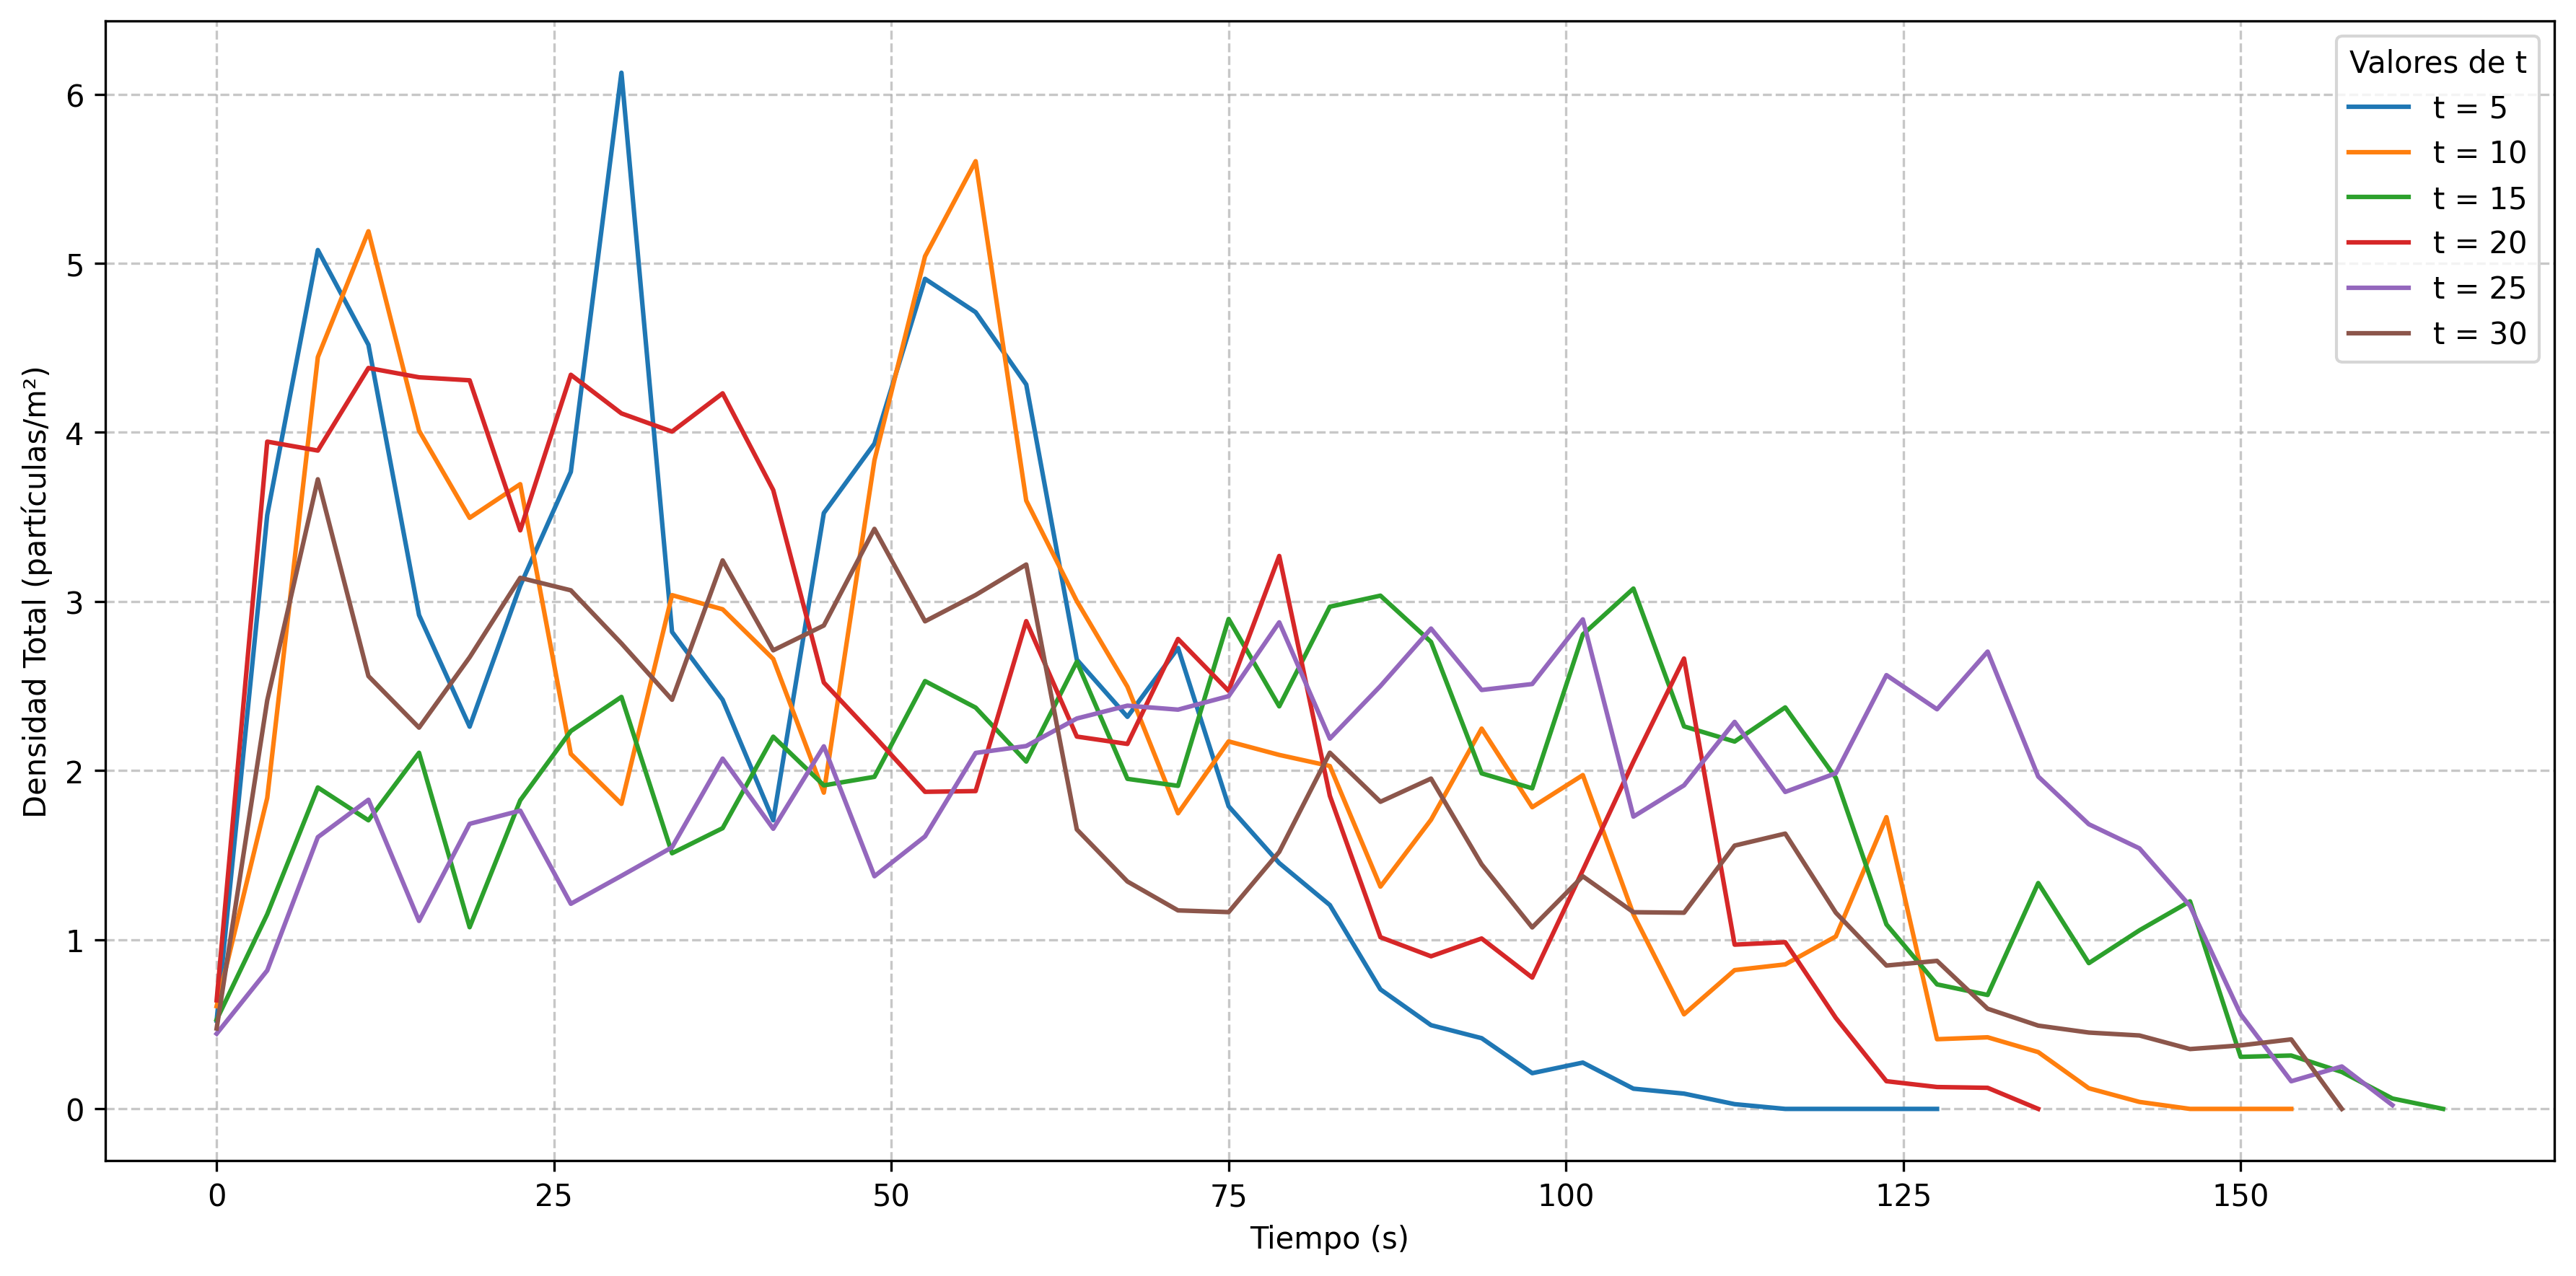
\includegraphics[width=0.9\textwidth]{img/density_vs_time_p0.50.png}
    \caption{Densidad en función del tiempo para $p=0,5$}
    \label{fig:flow_p100}
\end{figure}

\begin{figure}[H]
    \centering
    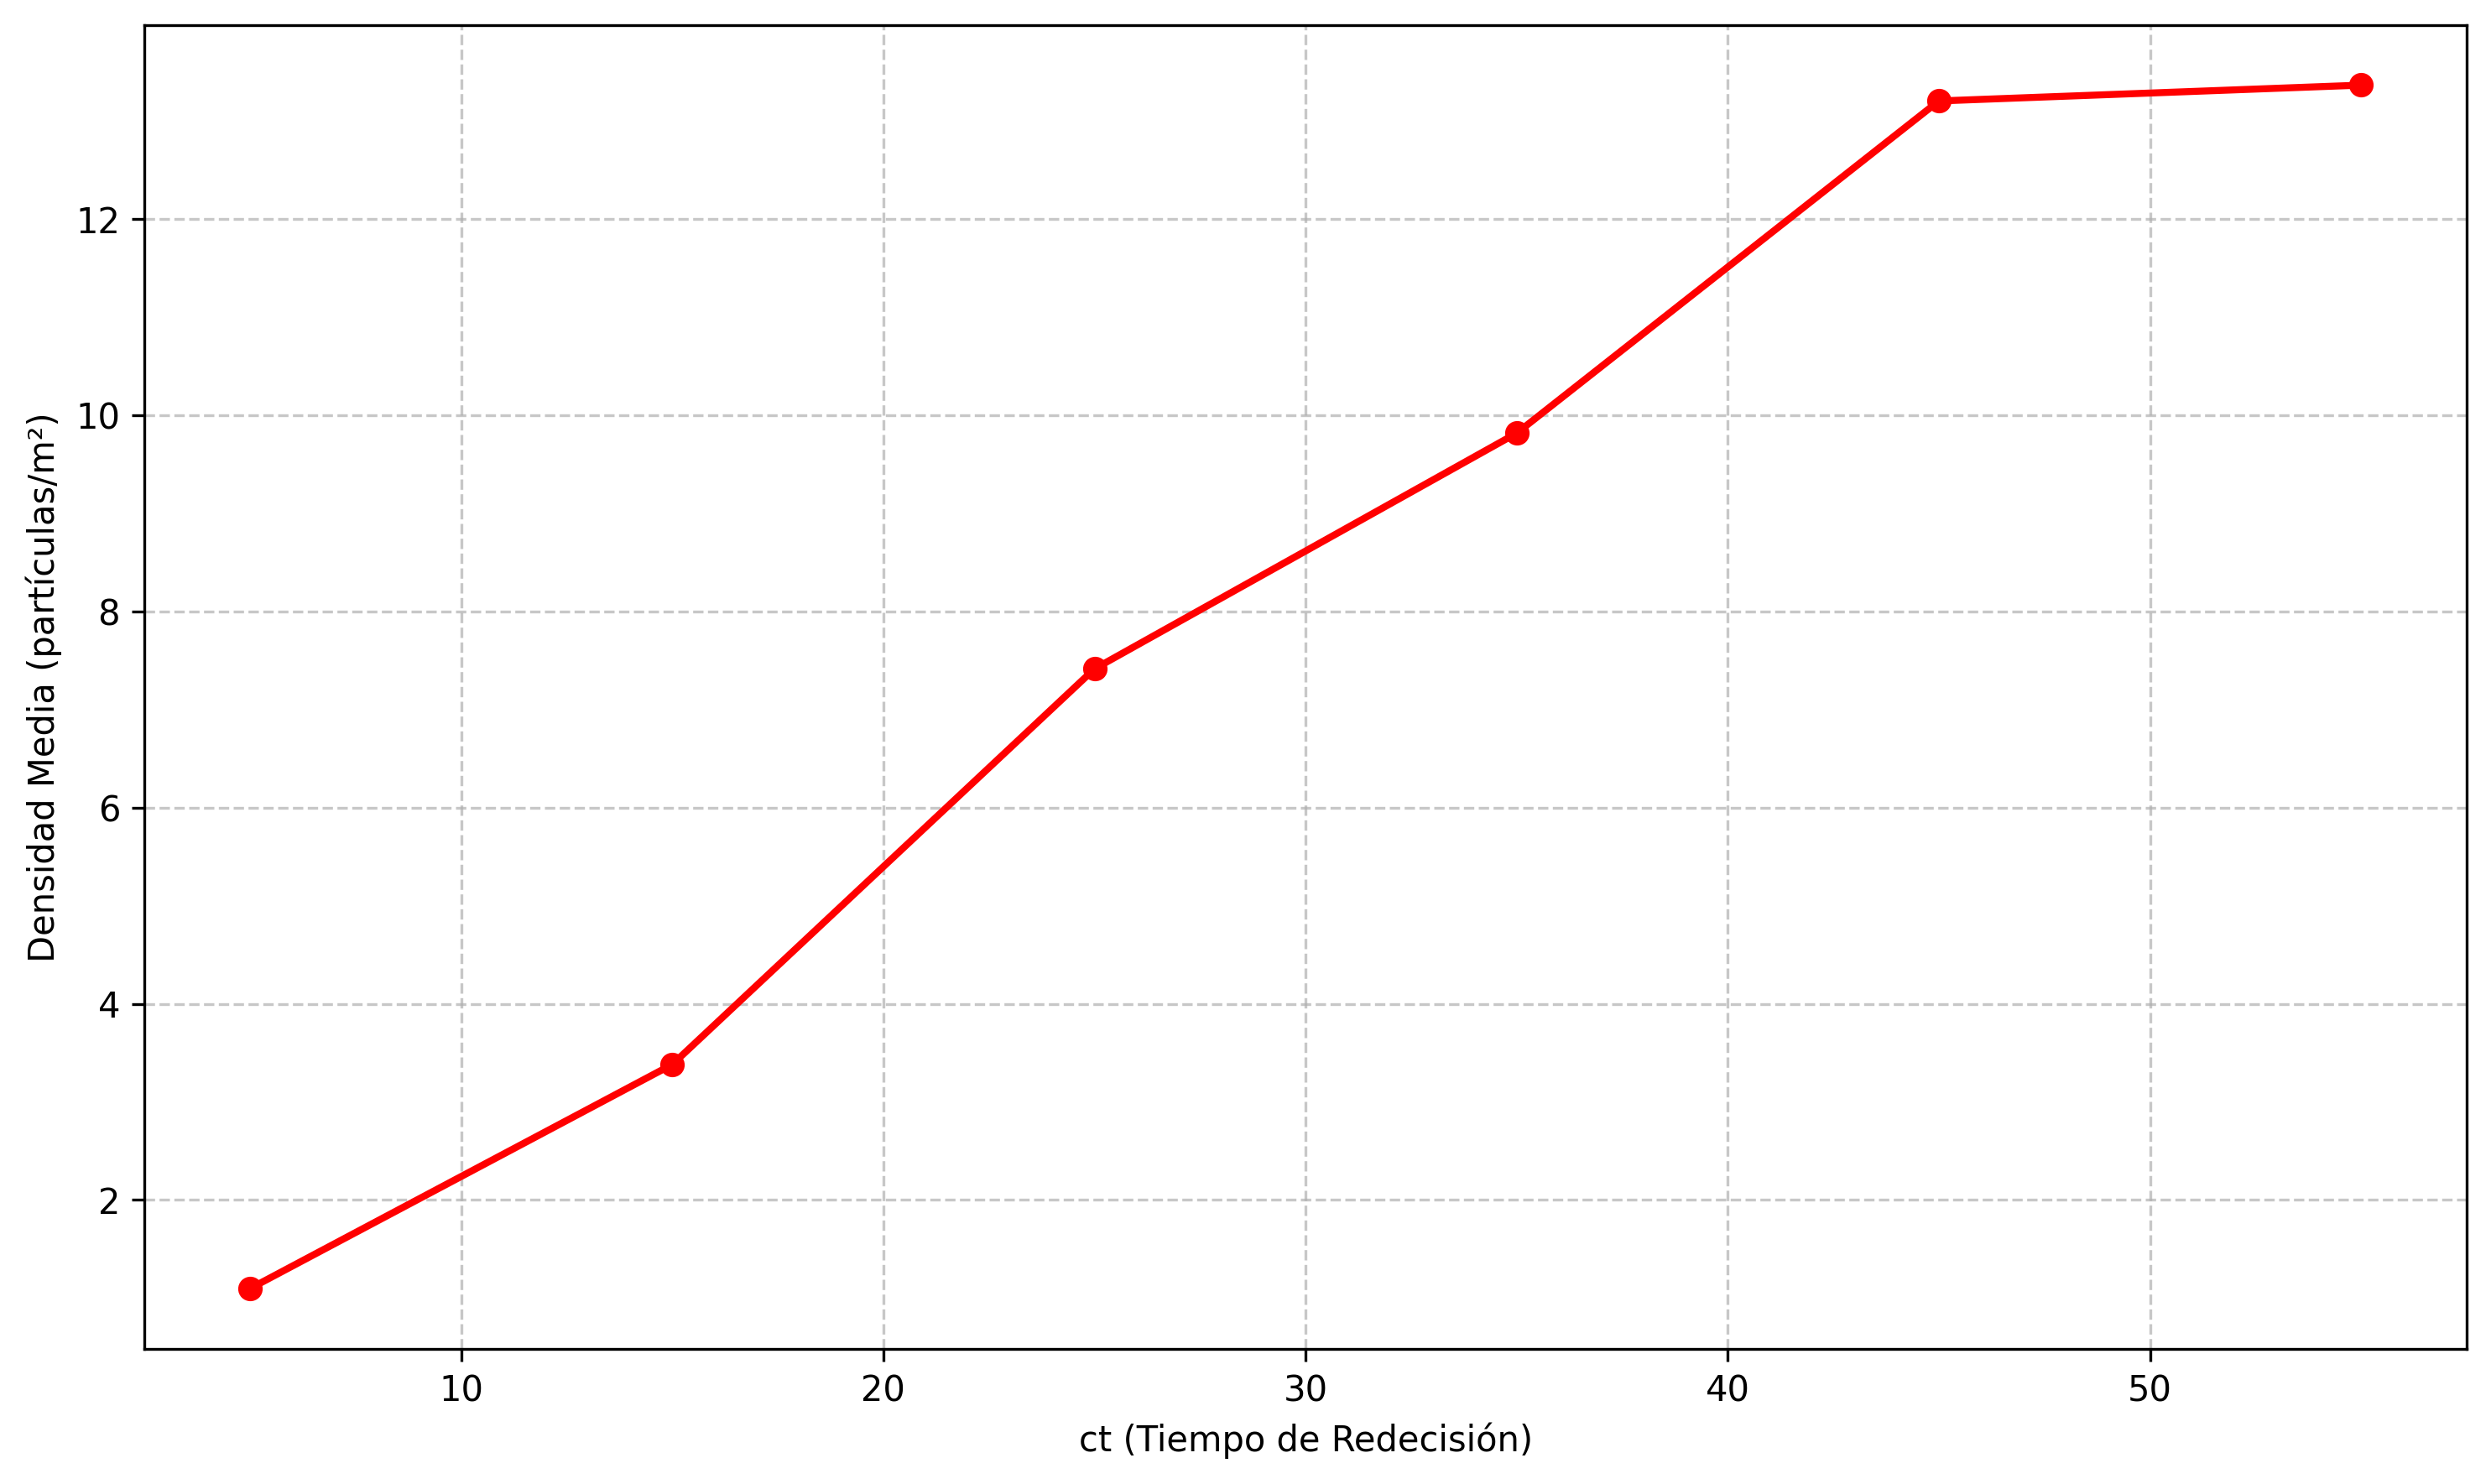
\includegraphics[width=0.9\textwidth]{img/average_density_p0.50.png}
    \caption{Densidad media en función de $ct$ para $p=0,5$}
    \label{fig:flow_p100}
\end{figure}

Se puede observar que a medida que aumenta el tiempo de re-decisión ($ct$), los agentes completan la evacuación en un tiempo menor. También notamos que la densidad media en las puertas es mayor conforme el tiempo que tardan para volver a evaluar su elección aumenta. Esto ocurre ya que a mayor $ct$, se quedan más tiempo en la puerta previamente elegida, lo que lleva a que se agrupen más los agentes.

\subsubsection{Coeficiente de uniformidad en función de $ct$}

\begin{figure}[H]
    \centering
    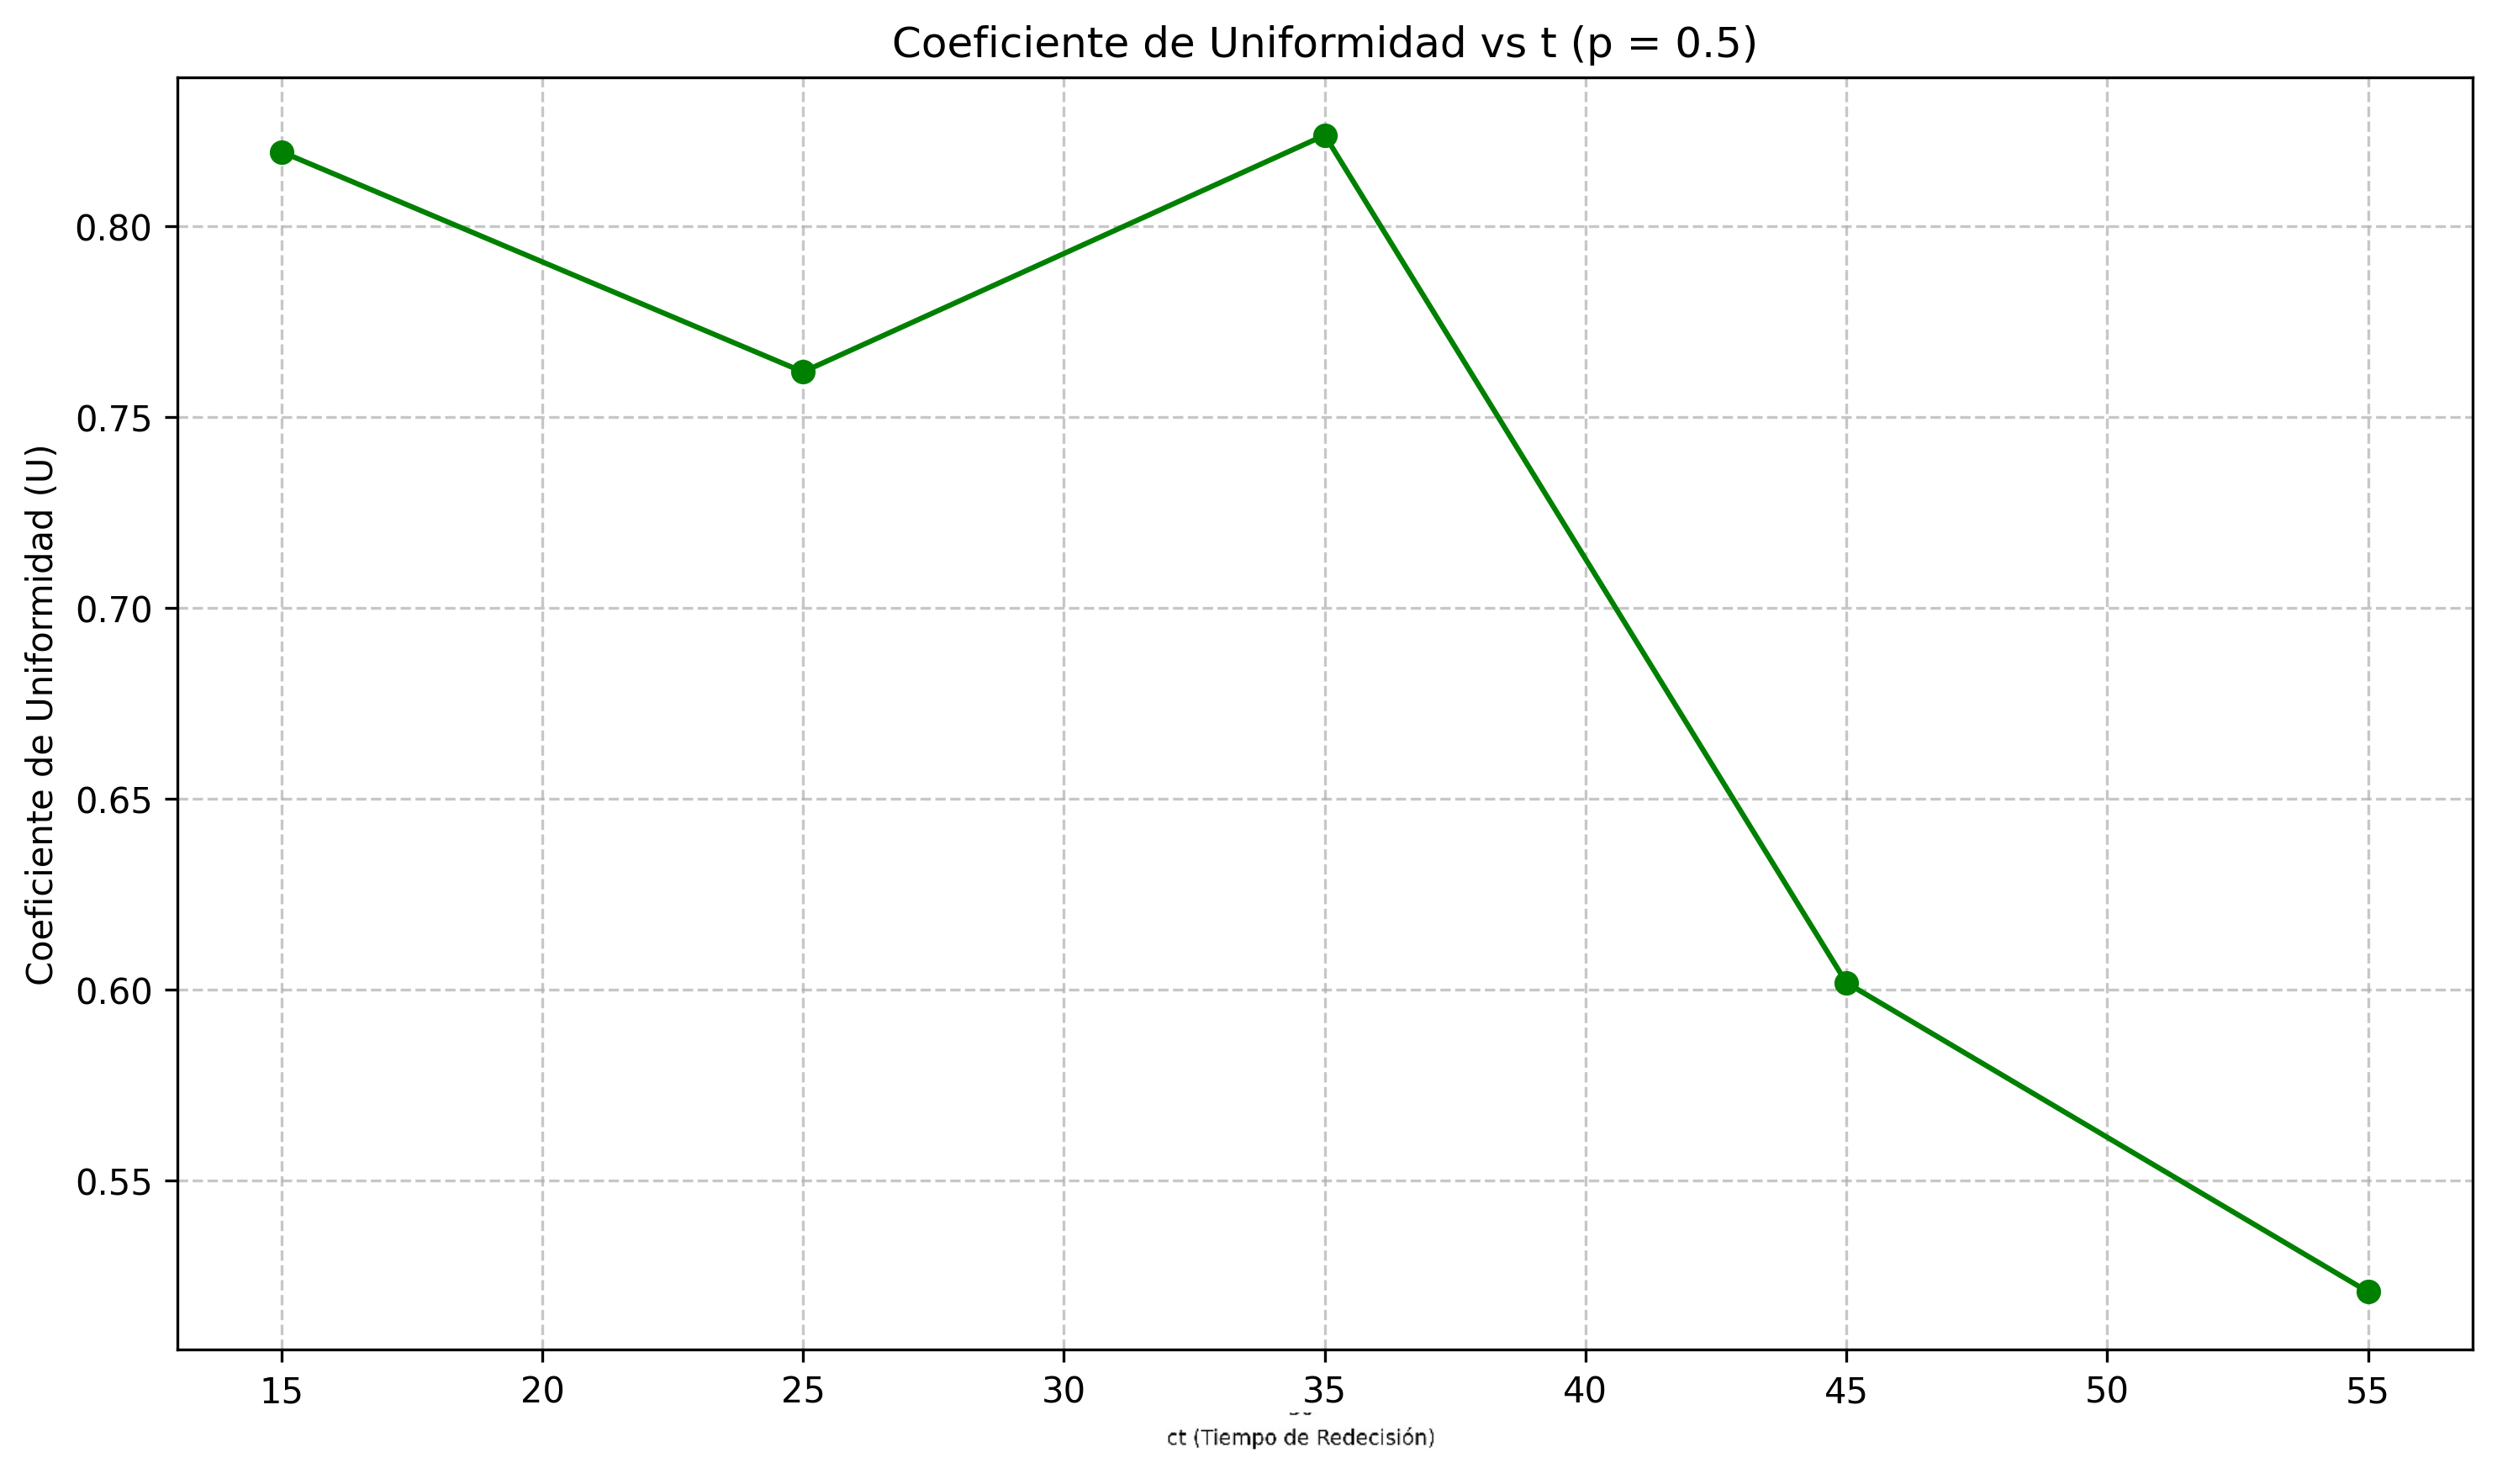
\includegraphics[width=0.9\textwidth]{img/uniformity_vs_t_p0.5.png}
    \caption{Coeficiente de uniformidad para $p=0,5$}
    \label{fig:flow_p100}
\end{figure}
Se puede ver que a medida que aumentamos el tiempo de re-decisión, el coeficiente de uniformidad disminuye. Esto se debe a que al volver a evaluar la elección de la puerta cada un tiempo alto, los agentes no reaccionan tanto a los cambios en la densidad de las puertas, por ende se van agrupando y no se reorganizan rápidamente si las densidades en las demás puertas varían. Por el contrario, si el tiempo de re-decisión es mas pequeño, las partículas notan rápidamente los cambios en las densidades de las puertas y pueden cambiar su elección para salir de forma más ordenada y utilizar las puertas por igual.

\section{Conclusiones}
[Sección para completar con las conclusiones]

\section{Referencias}
[1] Baglietto, G., Parisi, D. R. (2011). Continuous-space automaton model for pedestrian dynamics. Physical Review E, 83(5), 056117.
\end{document}


